% Template of basic phisics experiment 基于 article template，在此基础上做修改
% 设定文章编码类型，正文字号为五号则 zihao=5，正文字号为小四则 zihao=-4
\documentclass[zihao=5, UTF8]{article}		


% 自定义宏定义
\def\N{\mathbb{N}}
\def\F{\mathbb{F}}
\def\Z{\mathbb{Z}}
\def\Q{\mathbb{Q}}
\def\R{\mathbb{R}}
\def\C{\mathbb{C}}
\def\T{\mathbb{T}}
\def\S{\mathbb{S}}
\def\A{\mathbb{A}}
\def\I{\mathscr{I}}
\def\d{\mathrm{d}}
\def\p{\partial}


% 物理实验报告所需的其它宏包
\usepackage{ulem}   % \uline 下划线支持

% 导入基本宏包
\usepackage[UTF8]{ctex}     % 设置文档为中文语言
\usepackage[colorlinks, linkcolor=blue, anchorcolor=blue, citecolor=blue, urlcolor=blue]{hyperref}  % 宏包：自动生成超链接 (此宏包与标题中的数学环境冲突)
% \usepackage{docmute}    % 宏包：子文件导入时自动去除导言区，用于主/子文件的写作方式，\include{./51单片机笔记}即可。注：启用此宏包会导致.tex文件capacity受限。
\usepackage{amsmath}    % 宏包：数学公式
\usepackage{mathrsfs}   % 宏包：提供更多数学符号
\usepackage{amssymb}    % 宏包：提供更多数学符号
\usepackage{pifont}     % 宏包：提供了特殊符号和字体
\usepackage{extarrows}  % 宏包：更多箭头符号

% 列表环境设置
\usepackage{enumitem}   % 宏包：列表环境设置
    \setlist[enumerate]{itemsep=0pt, parsep=0pt, topsep=0pt, partopsep=0pt, leftmargin=3.5em} 
    \setlist[itemize]{itemsep=0pt, parsep=0pt, topsep=0pt, partopsep=0pt, leftmargin=3.5em}
    \newlist{circledenum}{enumerate}{1} % 创建一个新的枚举环境  
    \setlist[circledenum,1]{  
        label=\protect\circled{\arabic*}, % 使用 \arabic* 来获取当前枚举计数器的值，并用 \circled 包装它  
        ref=\arabic*, % 如果需要引用列表项，这将决定引用格式（这里仍然使用数字）
        itemsep=0pt, parsep=0pt, topsep=0pt, partopsep=0pt, leftmargin=3.5em
    }  
% 文章页面 margin 设置
\usepackage[a4paper]{geometry}  % 宏包：文章页面 margin 设置
    \geometry{top=0.75in}
    \geometry{bottom=0.75in}
    \geometry{left=0.75in}
    \geometry{right=0.75in}   % 设置上下左右页边距
    \geometry{marginparwidth=1.75cm}    % 设置边注距离（注释、标记等）

% 自定义数学环境
\usepackage{amsthm} % 宏包：数学环境配置
% theorem-line 环境自定义
    \newtheoremstyle{MyLineTheoremStyle}% <name>
        {11pt}% <space above>
        {11pt}% <space below>
        {}% <body font> 使用默认正文字体
        {}% <indent amount>
        {\bfseries}% <theorem head font> 设置标题项为加粗
        {：}% <punctuation after theorem head>
        {.5em}% <space after theorem head>
        {\textbf{#1}\thmnumber{#2}\ \ (\,\textbf{#3}\,)}% 设置标题内容顺序
    \theoremstyle{MyLineTheoremStyle} % 应用自定义的定理样式
    \newtheorem{LineTheorem}{Theorem.\,}
% theorem-block 环境自定义
    \newtheoremstyle{MyBlockTheoremStyle}% <name>
        {11pt}% <space above>
        {11pt}% <space below>
        {}% <body font> 使用默认正文字体
        {}% <indent amount>
        {\bfseries}% <theorem head font> 设置标题项为加粗
        {：\\ \indent}% <punctuation after theorem head>
        {.5em}% <space after theorem head>
        {\textbf{#1}\thmnumber{#2}\ \ (\,\textbf{#3}\,)}% 设置标题内容顺序
    \theoremstyle{MyBlockTheoremStyle} % 应用自定义的定理样式
    \newtheorem{BlockTheorem}[LineTheorem]{Theorem.\,} % 使用 LineTheorem 的计数器
% definition 环境自定义
    \newtheoremstyle{MySubsubsectionStyle}% <name>
        {11pt}% <space above>
        {11pt}% <space below>
        {}% <body font> 使用默认正文字体
        {}% <indent amount>
        {\bfseries}% <theorem head font> 设置标题项为加粗
        {：\\ \indent}% <punctuation after theorem head>
        {0pt}% <space after theorem head>
        {\textbf{#3}}% 设置标题内容顺序
    \theoremstyle{MySubsubsectionStyle} % 应用自定义的定理样式
    \newtheorem{definition}{}


% 有色文本框及其设置
\usepackage[dvipsnames,svgnames]{xcolor}    %设置插入的文本框颜色
\usepackage[strict]{changepage}     % 提供一个 adjustwidth 环境
\usepackage{framed}     % 实现方框效果
    \definecolor{graybox_color}{rgb}{0.95,0.95,0.96} % 文本框颜色。修改此行中的 rgb 数值即可改变方框纹颜色，具体颜色的rgb数值可以在网站https://colordrop.io/ 中获得。（截止目前的尝试还没有成功过，感觉单位不一样）（找到喜欢的颜色，点击下方的小眼睛，找到rgb值，复制修改即可）
    \newenvironment{graybox}{%
    \def\FrameCommand{%
    \hspace{1pt}%
    {\color{gray}\small \vrule width 2pt}%
    {\color{graybox_color}\vrule width 4pt}%
    \colorbox{graybox_color}%
    }%
    \MakeFramed{\advance\hsize-\width\FrameRestore}%
    \noindent\hspace{-4.55pt}% disable indenting first paragraph
    \begin{adjustwidth}{}{7pt}%
    \vspace{2pt}\vspace{2pt}%
    }
    {%
    \vspace{2pt}\end{adjustwidth}\endMakeFramed%
    }

% 各级标题自定义设置
\usepackage{titlesec}   
    % section标题自定义设置 
    \titleformat{\section}[hang]{\normalfont\huge\bfseries\centering}{第\,\thesection\,部分}{20pt}{}
    % subsection标题自定义设置 
    \titleformat{\subsection}[hang]{\normalfont\Large\bfseries}{\,\thesubsection\,}{8pt}{}
    % subsubsection标题自定义设置
    \titleformat{\subsubsection}[hang]{\normalfont\large\bfseries}{\,\thesubsubsection\,}{6pt}{}

% 外源代码插入设置
\usepackage{matlab-prettifier}
    \lstset{
        style=Matlab-editor,  % 继承matlab代码颜色等
    }
\usepackage[most]{tcolorbox} % 引入tcolorbox包 
\usepackage{listings} % 引入listings包
    \tcbuselibrary{listings, skins, breakable}
    \lstdefinestyle{matlabstyle}{
        language=Matlab,
        basicstyle=\small,
        breakatwhitespace=false,
        breaklines=true,
        captionpos=b,
        keepspaces=true,
        numbers=left,
        numbersep=15pt,
        showspaces=false,
        showstringspaces=false,
        showtabs=false,
        tabsize=2
    }
    \newtcblisting{matlablisting}{
        arc=0pt,
        top=0pt,
        bottom=0pt,
        left=1mm,
        listing only,
        listing style=matlabstyle,
        breakable,
        colback=white   % 选一个合适的颜色
    }

% table 支持
\usepackage{booktabs}   % 宏包：三线表
\usepackage{tabularray} % 宏包：表格排版
\usepackage{longtable}  % 宏包：长表格
\usepackage{tabularx}  % 宏包：宽表格
\usepackage{multirow}  % 宏包：表格中一格显示多个项目

% figure 设置
\usepackage{graphicx}  % 支持 jpg, png, eps, pdf 图片 
\usepackage{subcaption}    % 支持子图
\usepackage{svg}       % 支持 svg 图片
    \svgsetup{
        % 指向 inkscape.exe 的路径
        inkscapeexe = C:/aa_MySame/inkscape/bin/inkscape.exe, 
        % 一定程度上修复导入后图片文字溢出几何图形的问题
        inkscapelatex = false                 
    }


% 图表进阶设置
\usepackage{float}     % 图表位置浮动设置 
\usepackage{caption}    % 图注、表注
    \captionsetup[figure]{name=图}  
    \captionsetup[table]{name=表}
    \captionsetup{labelfont=bf, font=small}

% 文章默认字体设置
    \usepackage{fontspec}   % 宏包：字体设置
       \setmainfont{SimSun}    % 设置中文字体为宋体字体
      \setCJKmainfont[AutoFakeBold=3]{SimSun} % 设置加粗字体为 SimSun 族，AutoFakeBold 可以调整字体粗细^     \setmainfont{Times New Roman} % 设置英文字体为Times New Roman


% 其它设置
    % equation 公式编号设置
        \makeatletter  
        \renewcommand{\theequation}{\thesection.\arabic{equation}}  
        \makeatother
    % 脚注设置
        \renewcommand\thefootnote{\ding{\numexpr171+\value{footnote}}}
    % 参考文献引用设置
        \bibliographystyle{unsrt}   % 设置参考文献引用格式为unsrt
        \newcommand{\upcite}[1]{\textsuperscript{\cite{#1}}}     % 自定义上角标式引用
    % 文章序言设置
        \newcommand{\cnabstractname}{序言}
        \newenvironment{cnabstract}{%
            \par\Large
            \noindent\mbox{}\hfill{\bfseries \cnabstractname}\hfill\mbox{}\par
            \vskip 2.5ex
            }{\par\vskip 2.5ex}


% 页眉页脚设置
\usepackage{fancyhdr}   %宏包：页眉页脚设置
    \pagestyle{fancy}
    \fancyhf{}
    \cfoot{\thepage}
    \renewcommand\headrulewidth{1pt}
    \renewcommand\footrulewidth{0pt}
    \rhead{\bfseries 分组序号: YK04-2}    
    \chead{《基础物理实验》实验报告,\ 韩初晓,\ 2023K8009908002}
    \lhead{2024.10.23}

% 文档信息设置
%\title{这里是标题\\The Title of the Report}
%\author{丁毅\\ \footnotesize 中国科学院大学，北京 100049\\ Yi Ding \\ %\footnotesize University of Chinese Academy of Sciences, Beijing %100049, China}
%\date{\footnotesize 2024.8 -- 2025.1}

% 开始编辑文章

\begin{document}
\noindent\begin{flushright}
    \zihao{2}{分组序号: YK04-2}
\end{flushright}

\setCJKfamilyfont{boldsong}[AutoFakeBold = {2.17}]{SimSun}
\newcommand*{\boldsong}{\CJKfamily{boldsong}}


\begin{center}\large
    \noindent{\Huge\bfseries\boldsong《基础物理实验》实验报告 }
    \\\vspace{0.4cm}
    \noindent\textit{
        \textbf{\boldsong 实验名称：}\uline{\hspace{1.7cm} 傅里叶光学基础\hspace{1.7cm}}\hspace{0.4cm} 
        指导教师：\uline{\hspace{1.0cm}王研\hspace{1.0cm}}}
    \\\vspace{0.1cm}
    \noindent\textit{
        姓名：\uline{\,\,\,韩初晓\,\,\,}\hspace{0.2cm}
        学号：\uline{\,\,\,{\upshape 2023K8009908002}\,\,\,}\hspace{0.2cm}
        专业：\uline{\,\,\,计算机科学与技术\,\,\,}\hspace{0.2cm}
        班级：\uline{\,\,\,\upshape{2306}\,\,\,}}
    \\\vspace{0.1cm}
    \noindent\textit{
        实验日期：\uline{\,\,{\upshape 2024.10.23}\,\,}\hspace{0.2cm}
        实验地点：\uline{\,\,\,教学楼{\upshape705}\,\,\,}\hspace{0.2cm}
        是否调课/补课：\uline{\hspace{0.5cm}否\hspace{0.5cm}}\hspace{0.2cm}
        成绩：\uline{\hspace{2cm}}}
\end{center}
% \vspace{-0.2cm}
\noindent\rule{\textwidth}{0.1em}   % 分割线

% 控制目录不换页
\vspace{1cm}
\setcounter{tocdepth}{2}  % 目录深度为 2（不显示 subsubsection）
\noindent\begin{minipage}{\textwidth}\centering
\tableofcontents\thispagestyle{fancy}   % 显示页码、页眉等   
\end{minipage}  
\newpage

\section{阿贝成像与基本空间滤波}\thispagestyle{fancy} 

\subsection{实验原理}
阿贝成像将成像过程视为两步：

\begin{enumerate}
    \item \textbf{光场衍射}：入射光场在物平面上衍射，形成携带物信息的衍射场。这一衍射场在频谱面上形成频谱斑，反映了物信息与光场的卷积结果。
    
    \item \textbf{干涉成像}：这些频谱斑作为新的相干光源，发射球面波，经过光场传播后，在像平面上进行干涉，完成成像。
\end{enumerate}

\subsubsection{数学表述}

阿贝成像原理可以用以下公式表示：

1. \textbf{物波前}：
\begin{equation}
    u_{ob}(x, y) = A_1(t_0 + t_i \cos(2\pi f_i x))
\end{equation}

2. \textbf{频谱斑位置}：
\begin{equation}
    S_{\pm 1} = \pm F \tan(\theta_i), \quad \text{其中} \quad \sin(\theta_i) = \frac{f_i \lambda}{F}
\end{equation}

3. \textbf{相干光场复振幅}：
\begin{equation}
    A_0 \propto A_1 t_0 e^{ikL(B S_0)}, \quad A_{\pm 1} \propto \frac{1}{2} A_1 t_i e^{ikL(B S_{\pm 1})}
\end{equation}

4. \textbf{干涉像场}：
\begin{equation}
    u_{im}(x', y') = K e^{ik\frac{x'^2 + y'^2}{2z}} A_1(t_0 + t_i \cos(2\pi f'_i x'))
\end{equation}

\subsubsection{物理规律}

根据以上讨论，我们可以得到以下规律：

\begin{enumerate}
    \item 物原本的单频信息 $f_i$ 可以在像面重构为相似的但空间频率为 $f'_i$ 的信号，其比值 $V \equiv \frac{f'_i}{f_i}$ 就是放大率；
    
    \item 考虑到一个一般性的物是一系列 $f_i$ 的组合，因此在像面也会形成一个由 $f'_i$ 组合的像，其放大率为 $V$；
    
    \item 频谱面上的 $S_0$ 对应的就是物信息中的 0 频信息 $A_1 t_0$，其位置处于面内的源点；
    
    \item 正负两方向的衍射点 $S_{+1}$ 和 $S_{-1}$ 代表了指定频率 $f'_i$ 的信息 $A_1 t_i$，其位置由焦距 $F$ 和衍射角 $\theta_i$ 决定。空间频率 $f_i$ 越大，衍射角 $\theta_i$ 就越高，衍射点 $S_{+1}$ 和 $S_{-1}$ 离中心就越远。
\end{enumerate}


\subsection{实验仪器和用具}

\begin{center}
\begin{tabular}{|c|l|}
\hline
\textbf{组件名称} & \multicolumn{1}{c|}{\textbf{包含器件}} \\
\hline
激光器组件 & 激光器、棱镜夹持器、一维平移台、宽滑块、支杆和套筒 \\
\hline
扩束镜组件 & 凹透镜（Φ6，f=10mm）、透镜架、滑块、支杆和套筒 \\
\hline
准直镜组件 & 凸透镜（Φ40，f=80mm）、透镜架、滑块、支杆和套筒 \\
\hline
光栅字组件 & 光栅字（Φ40，10线/mm）、滑块、支杆和套筒 \\
\hline
变换透镜组件 & 凸透镜（Φ76，f=175mm）、镜架、滑块、支杆和套筒 \\
\hline
滤波器组件 & 滤波器（低通、方向滤波）、干板架、滑块、支杆和套筒 \\
\hline
白屏组件 & 白屏、干板架、滑块、支杆和套筒 \\
\hline
\end{tabular}
\captionof{table}{阿贝成像与基本空间滤波}
\end{center}


\subsection{实验内容}

\begin{enumerate}
    \item \textbf{光路布置和调节：}
    \begin{enumerate}
        \item 依次布置激光器组件、扩束镜组件、准直镜组件、光栅字组件、变换透镜组件、滤波器组件和白屏组件。相邻组件的纵向间隔参考值为：40mm、70mm、40mm、240mm、195mm和445mm。
        \item 安装激光器和白屏，调整激光器出光口至支杆顶部90mm，并使其沿导轨中心水平传播。调节白屏前后位置，确保激光在近处和远处均能打在白屏上同样高度。
        \item 安装扩束镜，调整支杆使扩束光斑中心与参考中心重合，然后固定。
        \item 安装准直镜，距扩束镜约70mm，调整支杆使平行光束与参考中心重合，然后固定。
        \item 安装光栅字，调整支杆使光斑正入射“光”字，位置尽量靠近准直镜。
        \item 安装变换透镜，调整支杆使入射“光”字通过透镜中心，移动透镜至白屏上见清晰的放大倒立实像，然后固定。
        \item 安装滤波器，前后移动以观察花样，固定在花样最清晰的位置。
        \item 测试不同滤波器，使用不同滤波器观察屏上的效果，确保不移动其他光学器件位置。
    \end{enumerate}

    \item \textbf{观察“光”栅字的像和频谱：}
    去掉滤波器，观察未滤波状态下的“光”字像，放大倍数足够大时可见横向与竖向条纹。实验中“光”字由空间频率12线/mm的光栅调制，通过变换透镜的频谱面放置屏幕可观察到频谱点。

    \item \textbf{观察方向滤波和低通滤波的实际效果：}
    \begin{enumerate}
        \item 选择“缝”滤波器，水平放置使0级点通过，观察到充满竖向条纹的像。
        \item 将“缝”旋转90度竖直放置，使0级点通过，观察到充满横向条纹的像。
        \item 将“缝”与光栅方向夹角放置45度，观察效果。
        \item 将“孔”放置在频谱面，仅让0级点通过，观察到“光”字轮廓。
    \end{enumerate}
\end{enumerate}

\subsection{实验效果}

\input{./abbe_imaging.tex}


\section{光学4F系统成像}

\subsection{实验原理}

\textbf{光学4F图像处理系统能解决单透镜成像系统的局限性。单透镜系统存在以下缺点：}
\begin{enumerate}
    \item 成像需求与频谱面处理需求可能冲突，可调节参数有限。例如，在假彩色编码实验中，若光源亮度不足，想要通过增大物与透镜的距离来提高像的亮度，可能导致物的衍射光超出透镜的尺寸，造成空间信息缺失。
    \item 单透镜成像时，像场函数与物场函数之间存在相位因子差异。在相干光学中，相位非常重要，保持处理后图像的相位一致性往往是必要的。
\end{enumerate}

\textbf{4F系统通过两个透镜实现傅里叶变换和反傅里叶变换，将成像和频谱处理分离，具有更好的可控性、保真性和稳定性。其工作原理如下：}
\begin{itemize}
    \item 物场函数位于第一个透镜（傅里叶变换透镜）的焦距处，因此其像面在无限远处，导致额外的相位因子转变为1。反傅里叶变换透镜仅将无限大的像整合到后焦面。
    \item 在无滤波且放大倍率为1时，4F系统的像场函数严格（包括相位）复制物场函数。
\end{itemize}

\textbf{具体过程如下：}
一束平行光照射透明物体，物体放置于第一个透镜的前焦面，第一透镜后焦面得到物函数的频谱 \(G(f_\xi, f_\eta)\)。该频谱面位于第二透镜的前焦面，经过第二透镜后，得到频谱函数的傅里叶变换 \(g(x, y)\)。物函数经过两次傅里叶变换后重新获得，但为倒像。为消除由于傅里叶变换引入的负号，像平面的坐标方向与物平面的方向相反。此外，在频谱面上插入空间滤波器可以改变频谱函数，从而实现信号处理。


\subsection{实验仪器和用具}

\begin{table}[htbp]
    \centering
    \label{tab:components}
    \begin{tabular}{|p{3cm}|p{12cm}|}
        \hline
        \textbf{组件名称} & \textbf{包含器件} \\ 
        \hline
        光源组件 & 半导体激光器（650nm）一维平移台、宽滑块、支杆和套筒 \\
        \hline
        准直镜组件 & 凹透镜（Ф6, f-9.8mm）、凸透镜（Ф25, f-80mm）、透镜架、滑块、支杆和套筒 \\
        \hline
        调制物组件 & 物板、干板架、滑块、支杆和套筒 \\
        \hline
        变换透镜组件 & 凸透镜（Ф40, f-150mm）2个、镜架、滑块、支杆和套筒 \\
        \hline
        滤波器组件 & 滤波器（低通、方向滤波）、精密平移台、干板夹、滑块、支杆和套筒 \\
        \hline
        白屏组件 & 白屏、干板架、滑块、支杆和套筒 \\
        \hline
    \end{tabular}
    \caption{光学4F系统成像}
\end{table}

\subsection{实验内容}

\begin{enumerate}
    \item \textbf{实验条件：} 在阿贝成像的基础上，激光器、扩束镜、准直镜和白屏保持不动。
    \item \textbf{安装物孔：} 将光栅字和带字白纸的物孔垂直安装到支架上，调整支杆使准直光斑中心正入射物孔，固定支杆，确保物孔尽可能靠近准直镜以减少光程，同时固定物孔支架滑块防止移动。
    \item \textbf{安装变换透镜1：} 在物孔后方放置变换透镜1（$f=150\text{mm}$），调整支杆使光从透镜中心通过并固定高度。尽量接近物孔并固定变换透镜1支撑滑块。
    \item \textbf{安装变换透镜2：} 在变换透镜1后方放置变换透镜2（$f=150\text{mm}$），调整支杆使光从透镜中心通过并固定高度。移动变换透镜2至距离变换透镜1两倍焦距的位置，并固定支撑滑块。确保两个变换透镜对称或对易放置，遵循“凹凸面对准平行光”的原则以减少像差。
    \item \textbf{观察成像：} 在白屏上观察成像特点，查看与物体等大的清晰物像，比较与阿贝成像时单透镜成像的区别。可以在频谱面上安装滤波器，观察像的变化。
\end{enumerate}

\subsection{实验效果}

\begin{figure}[H]
  \centering
  \begin{subfigure}[b]{0.45\textwidth}
    \centering
    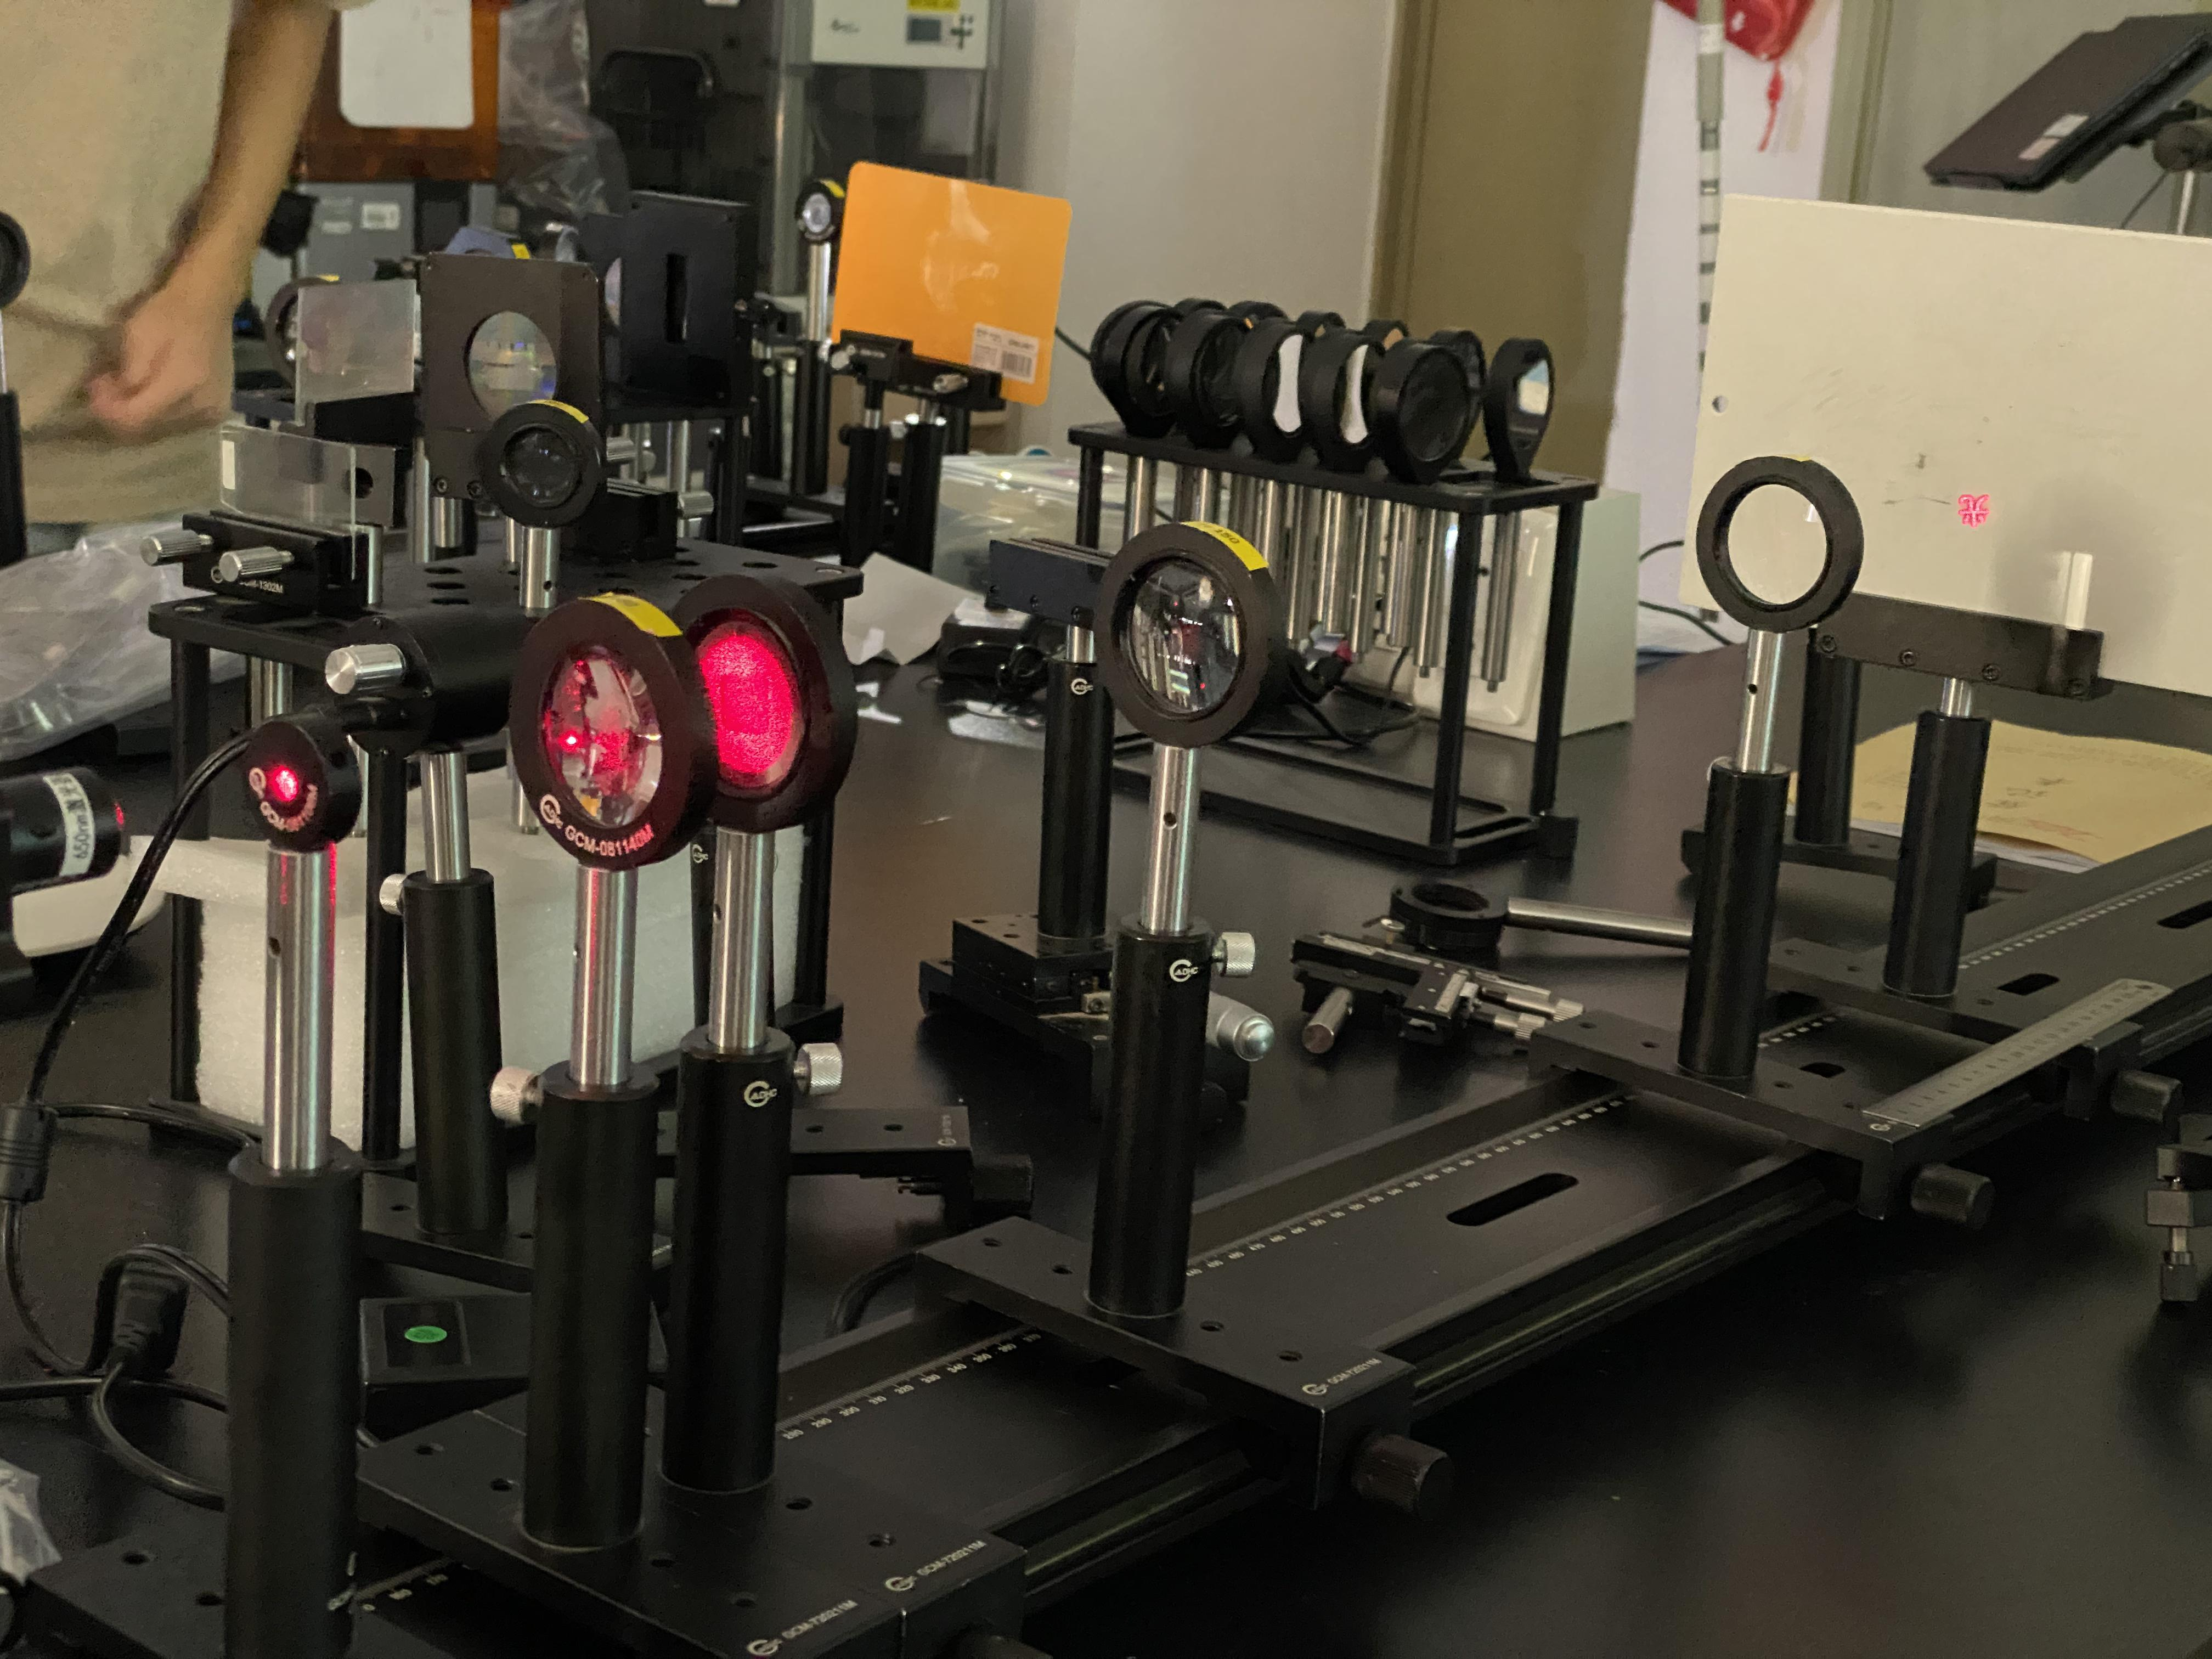
\includegraphics[height=5cm]{./pictures/photos/光学4F系统成像（光路图）.jpg}
    \caption{光学4F系统成像（光路图）}
    \label{fig:光学4F系统成像（光路图）}
  \end{subfigure}
  \hfill
  \begin{subfigure}[b]{0.45\textwidth}
    \centering
    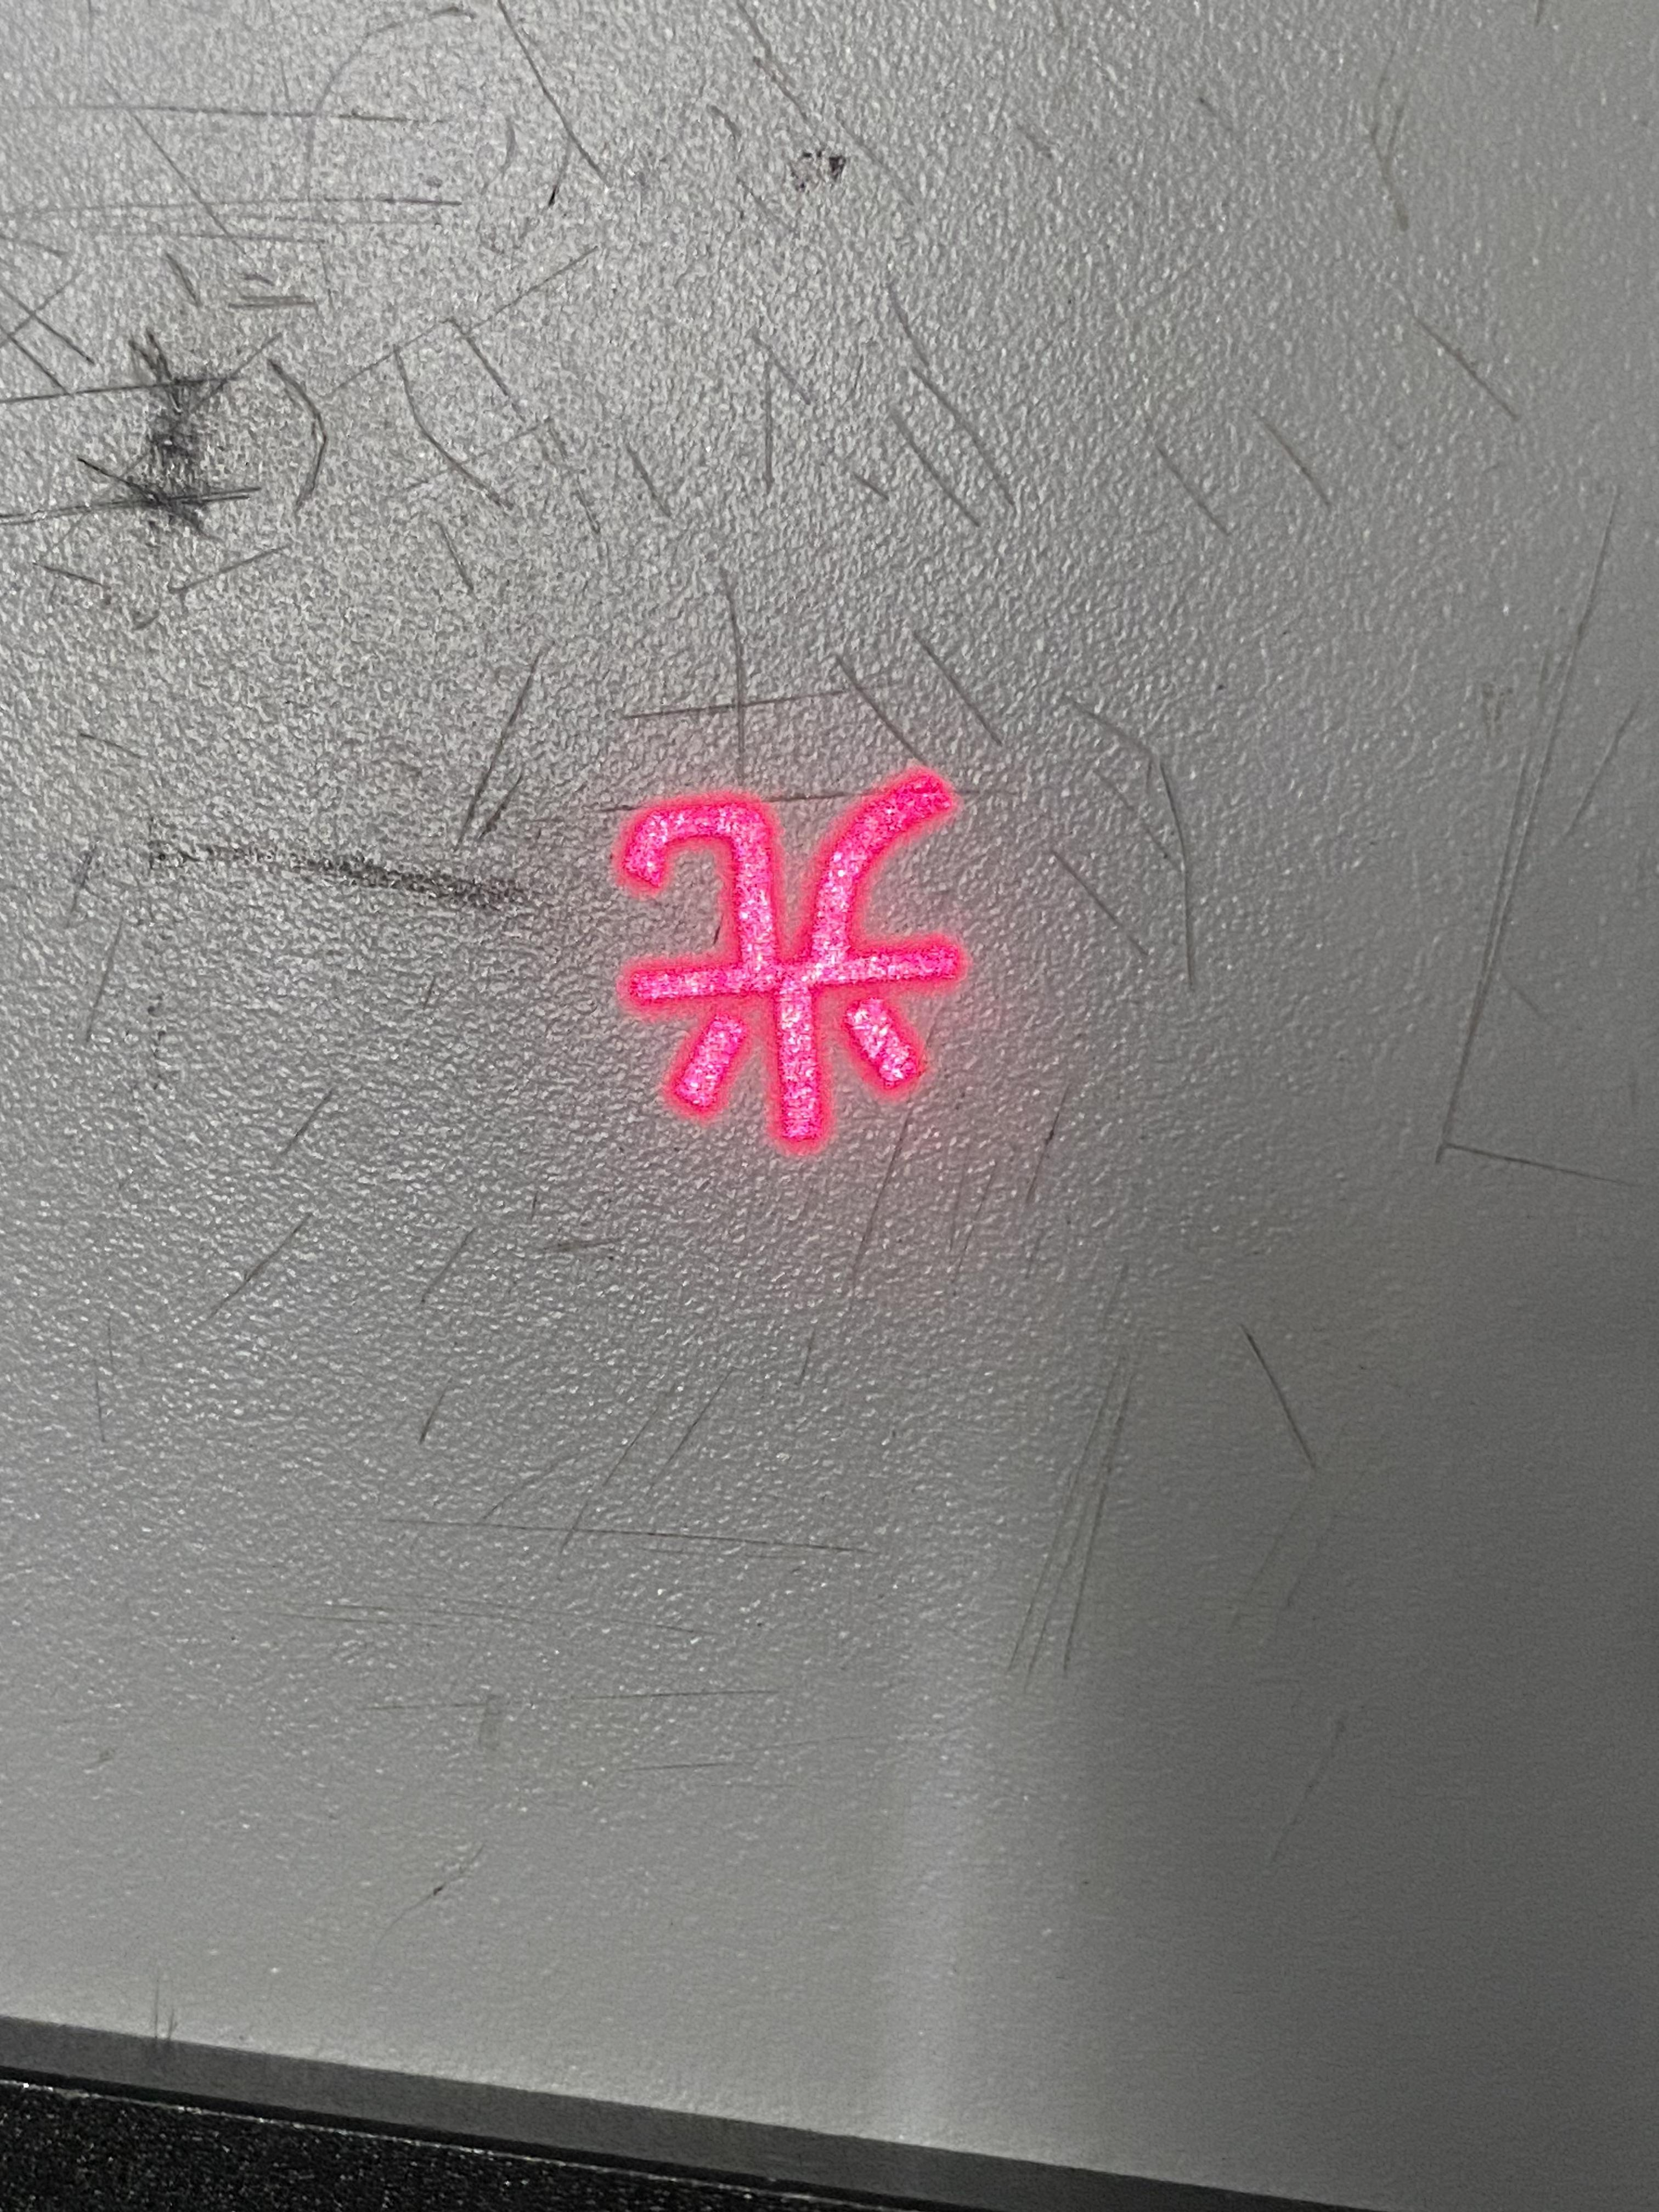
\includegraphics[height=5cm]{./pictures/photos/光栅字呈现出与物体等大的清晰物象.jpg}
    \caption{光栅字呈现出与物体等大的清晰物象}
    \label{fig:光栅字呈现出与物体等大的清晰物象}
  \end{subfigure}
  \label{fig:combined}
\end{figure}

\begin{figure}[H]
  \centering
  \begin{subfigure}[b]{0.45\textwidth}
    \centering
    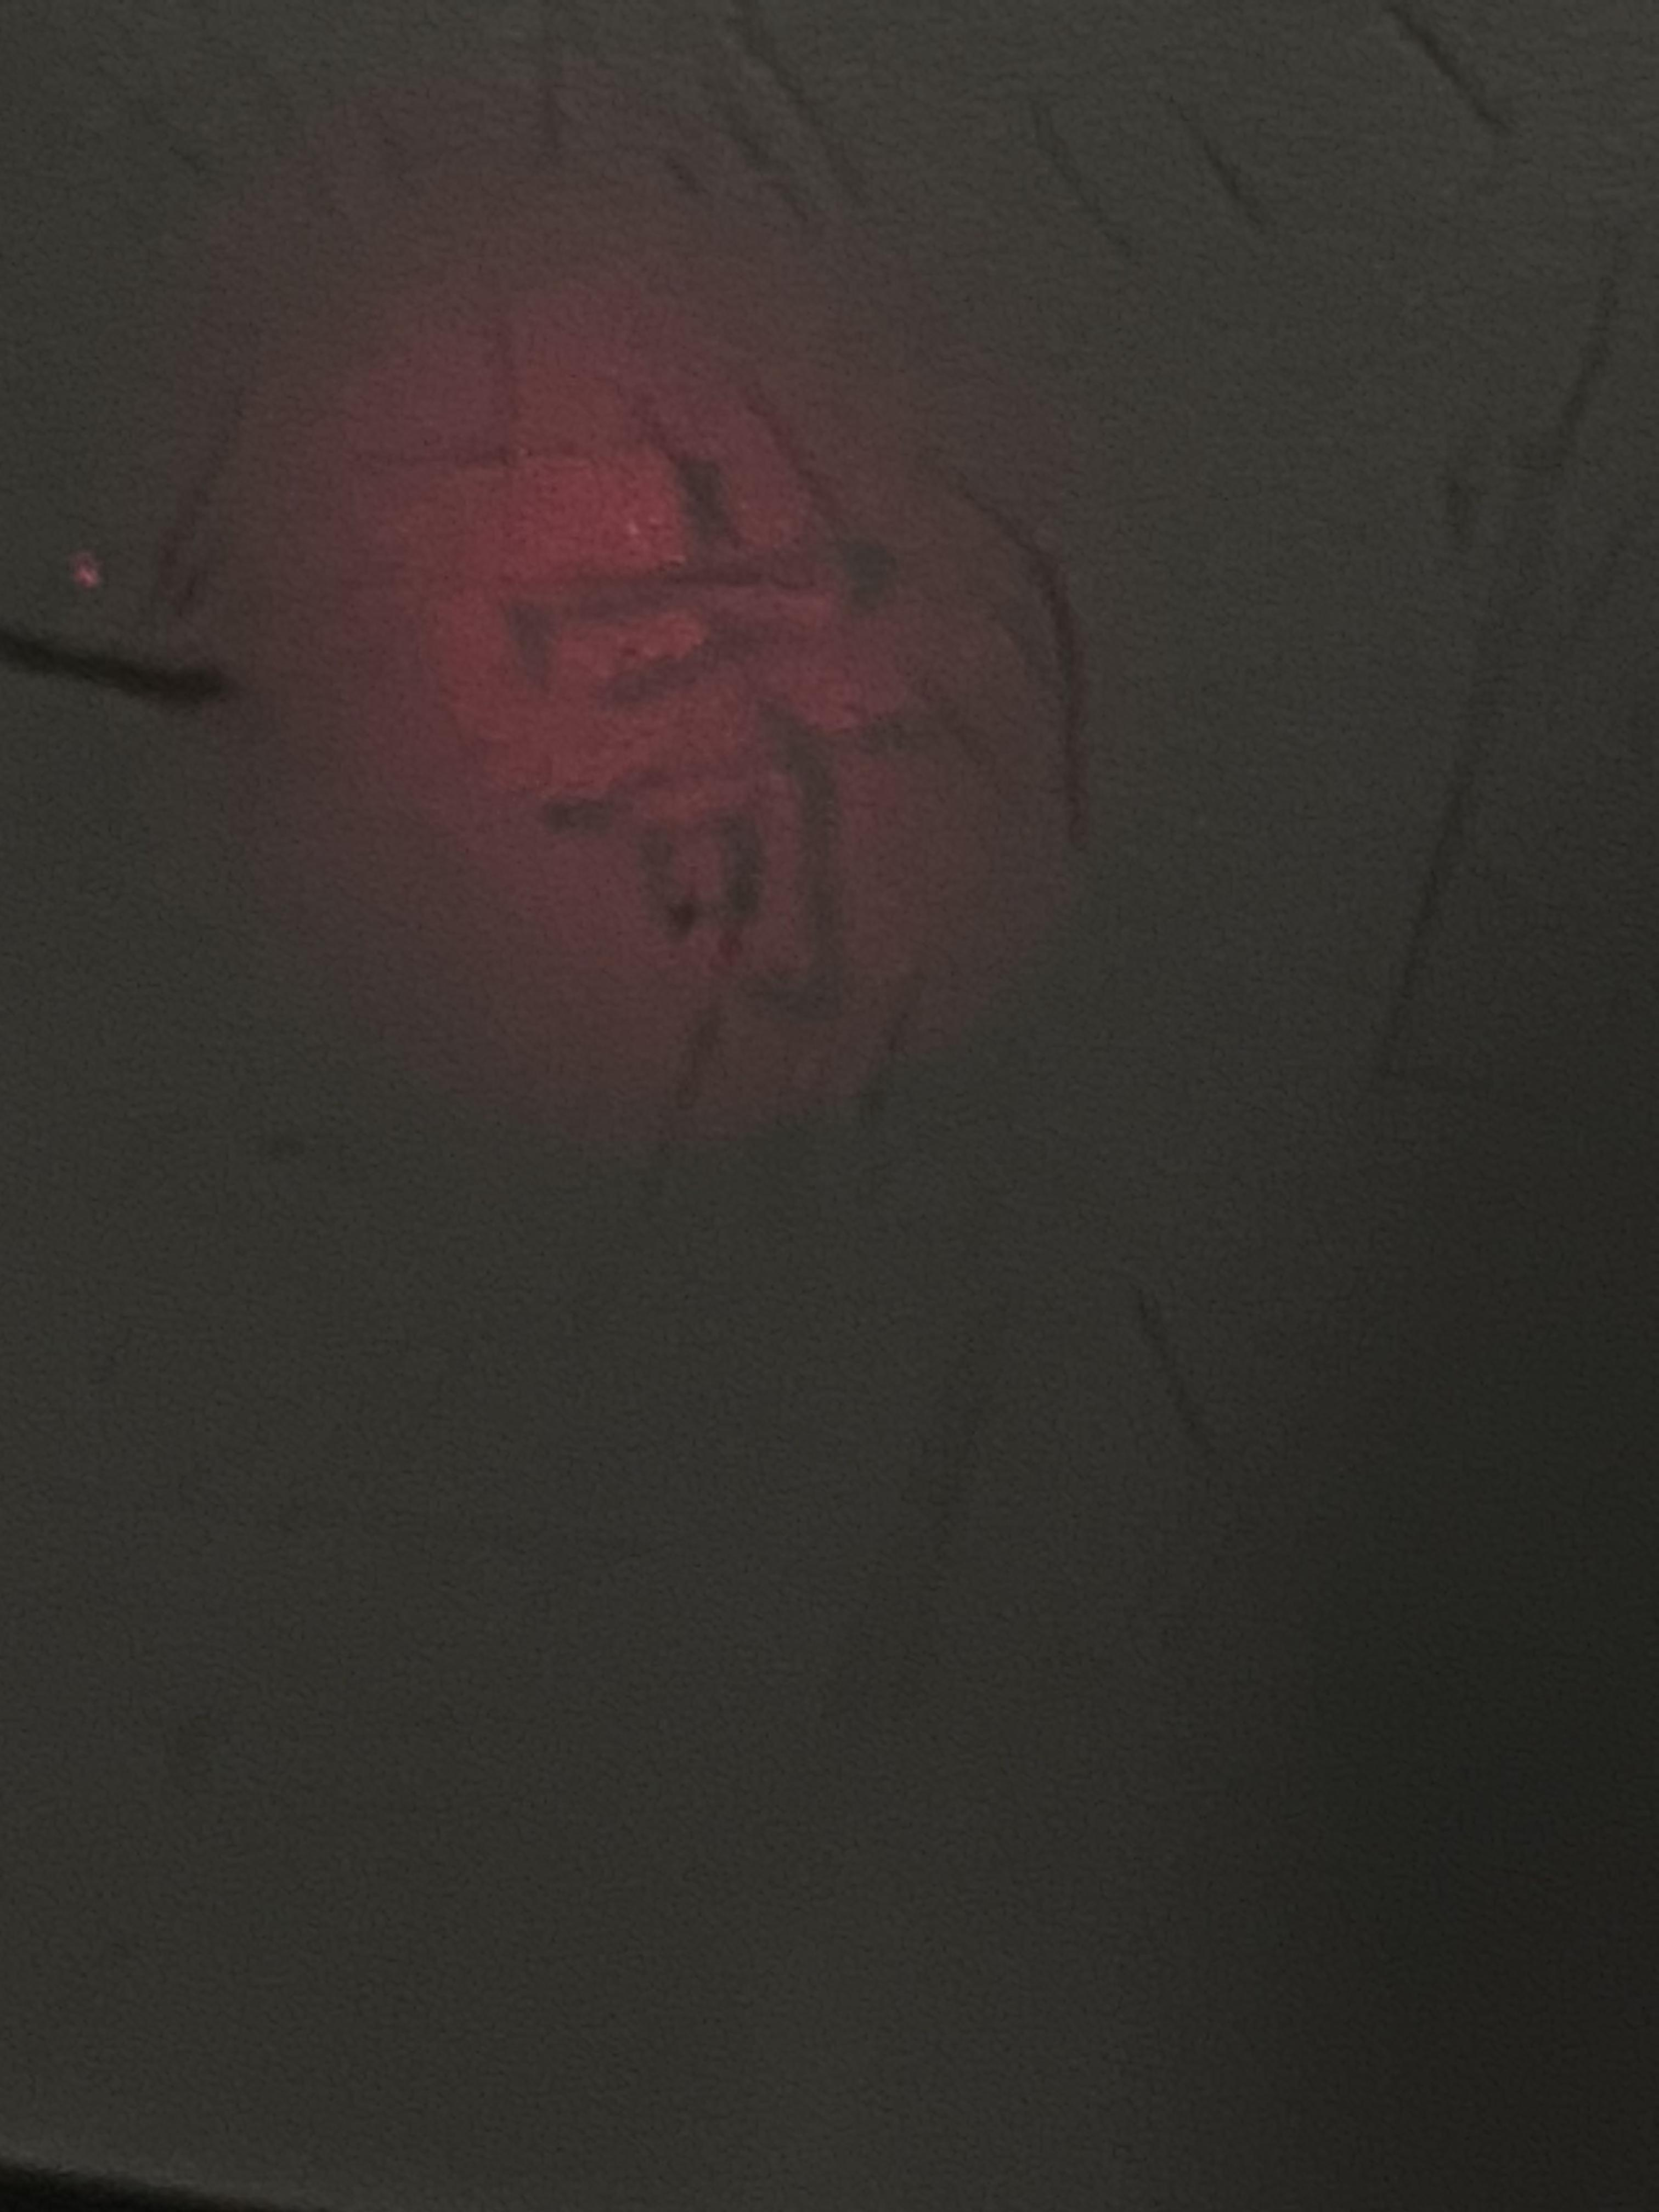
\includegraphics[height=5cm]{./pictures/photos/带字白纸呈现出与物体等大的清晰物象.jpg}
    \caption{带字白纸呈现出与物体等大的清晰物象}
    \label{fig:带字白纸呈现出与物体等大的清晰物象}
  \end{subfigure}
  \label{fig:combined}
\end{figure}


\section{假彩色编码}

\subsection{实验原理}

在假彩色编码实验中，可以使用白光光源照明一个预制了不同方向光栅的天安门图案，并通过颜色滤波器和自制空间选色滤波器，实现假彩色编码。

物样品天空、天安门和草地三个区域通过不同方向的光栅刻线调制，空间频率为 100 线/mm。白光照射透明天安门，因衍射行为，不同颜色的光将分散，形成多彩的衍射场；经过透镜汇聚，形成清晰的彩色频谱花样。不同区域的光栅方向导致衍射花样呈现出彩色带状分布。

可以选择：
\begin{enumerate}
    \item 使用三个不同方向、不同颜色（红、绿、蓝）的彩色滤片来过滤不同方向的衍射斑条纹；
    \item 使用一张白纸，在其上根据不同部位的衍射斑来选取指定的颜色通过。
\end{enumerate}

以上两种方法均可实现不同区域的彩色编码。由于该编码方法利用不同方位的光栅对图像不同空间部位进行调制，故称为 \textbf{θ调制空间假彩色编码}。实验能够在光屏上展现出绿草地、红天安门和蓝天。


\subsection{实验仪器和用具}

\begin{table}[h]
\centering
\begin{tabular}{|p{3cm}|p{10cm}|}
\hline
\textbf{组件名称} & \textbf{包含器件} \\
\hline
光源组件 & LED（650nm），一维平移台、宽滑块、支杆和套筒 \\
\hline
准直镜组件 & 凹透镜（Φ6，f-9.8mm）、凸透镜（Φ25，f-80mm）、透镜架、滑块、支杆和套筒 \\
\hline
调制物组件 & 天门光栅（100 线/mm）、干板架、滑块、支杆和套筒 \\
\hline
变换透镜组件 & 凸透镜（Φ40，f-150mm）2 个、镜架、滑块、支杆和套筒 \\
\hline
滤波器组件 & 滤波器（低通、方向滤波）、精密平移台、干板夹、滑块、支杆和套筒 \\
\hline
白屏组件 & 白屏、干板架、滑块、支杆和套筒 \\
\hline
\end{tabular}
\caption{假彩色编码}
\label{tab:components}
\end{table}

\subsection{实验内容}

\begin{enumerate}
    \item \textbf{光路布置和调节：}
    \begin{enumerate}
        \item 参照图10布置光路，自左向右依次为光源组件、准直镜组件、调制物组件、变换透镜组件、滤波器组件和白屏组件。相邻组件的水平方向间隔参考值为：80mm、40mm、275mm、160mm和335mm。
        \item 安装白光光源，调节LED光源支杆高度至约90mm（仅供参考）并固定。
        \item 安装白屏，将其固定在导轨右侧，尽量远离光源。
        \item 安装准直镜，距LED发光点约150mm，调整透镜高度使发光点与其中心对齐，并固定。水平调节透镜位置，确保在近处和远处光斑大小一致（注意色差），固定支撑滑块。
        \item 安装天安门光栅，调整支杆使光斑正入射其中心并固定。
        \item 安装变换透镜，调整支杆使光从透镜中心通过，移动透镜至白屏上见放大倒立实像后固定。
        \item 安装滤波器支架，安装纸片或铁片，并水平移动支架观察衍射光斑，直到出现清晰的频谱面花样，固定支架水平位置。后续使用不同滤波器进行滤波。
    \end{enumerate}

    \item \textbf{θ调制及现象观察：}
    \begin{enumerate}
        \item 使用θ调制滤波器，根据需要的颜色安装滤波器，并调整位置，使三色滤片与频谱面花样的指定分支匹配，观看经编码得到的假彩色像。
        \item 使用自制滤波器，找一张硬纸片标记三个方向需滤波的颜色，并在标记点扎孔。若LED光源的绿光成分弱，可考虑提取黄颜色代替。
    \end{enumerate}
\end{enumerate}

\subsection{实验效果}

\begin{figure}[H]
  \centering
  \begin{subfigure}[b]{0.45\textwidth}
    \centering
    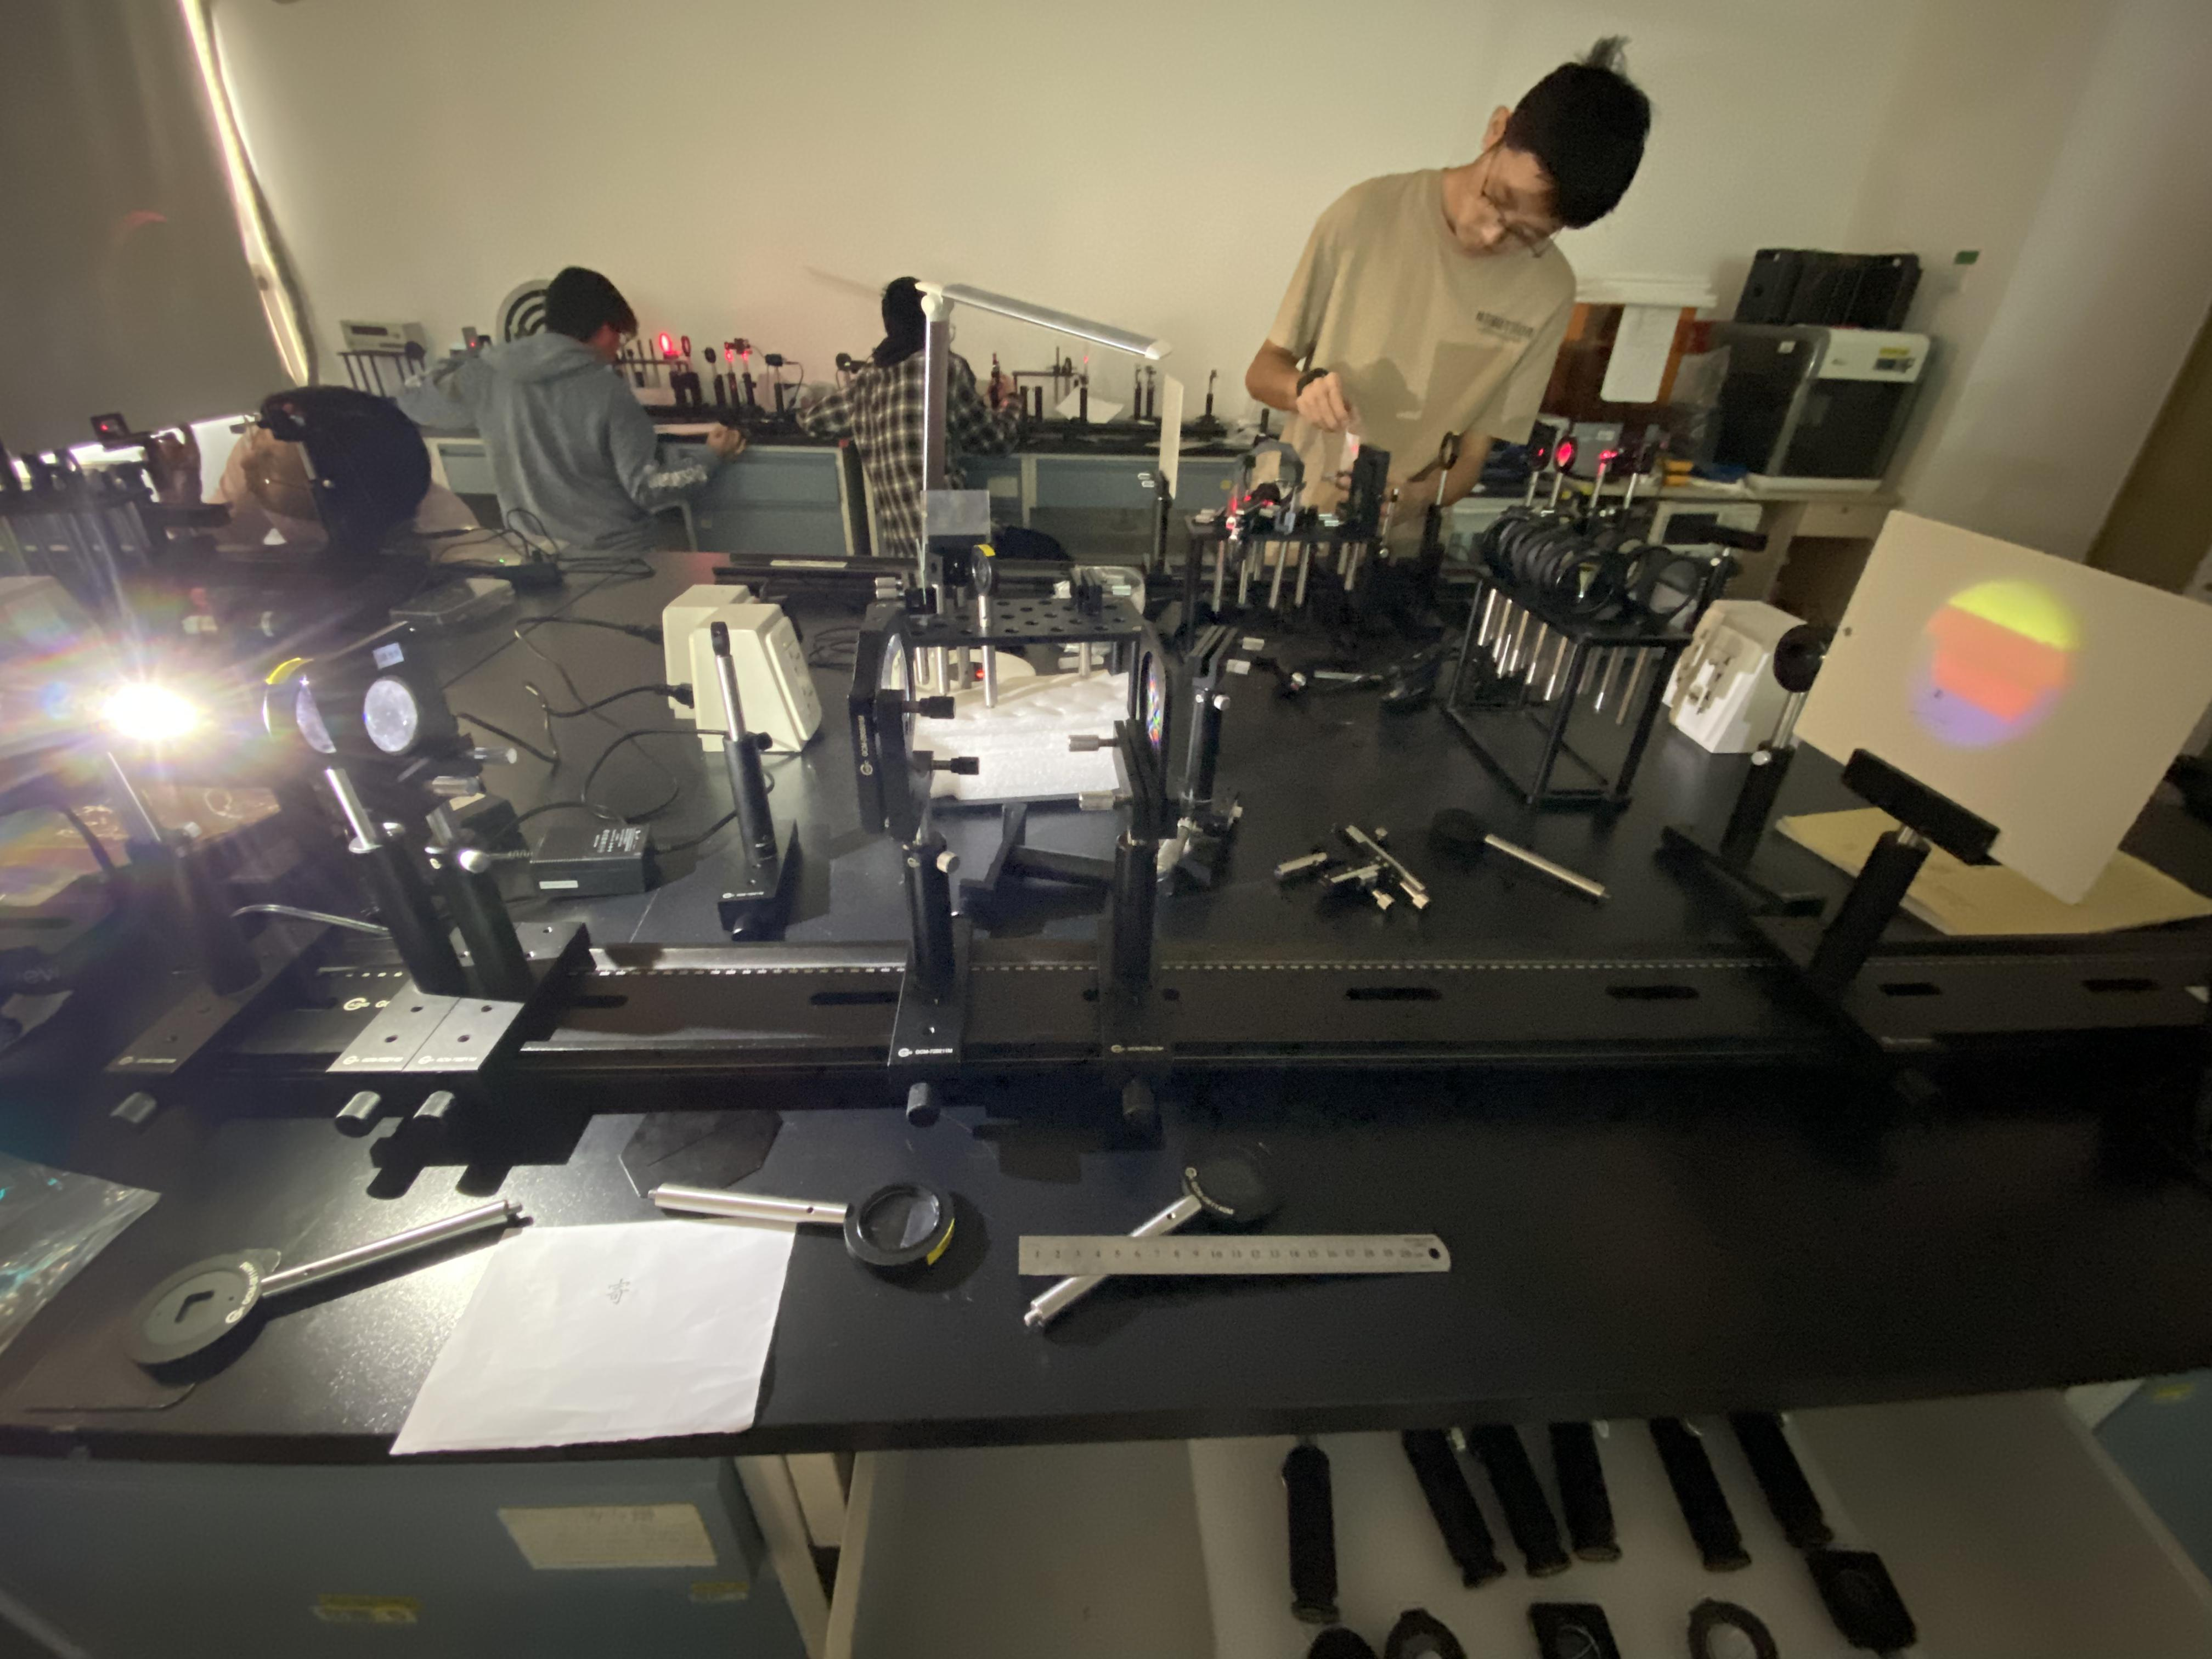
\includegraphics[height=5cm]{./pictures/photos/假彩色编码（光路图）.jpg}
    \caption{假彩色编码（光路图）}
    \label{fig:假彩色编码（光路图）}
  \end{subfigure}
  \hfill
  \begin{subfigure}[b]{0.45\textwidth}
    \centering
    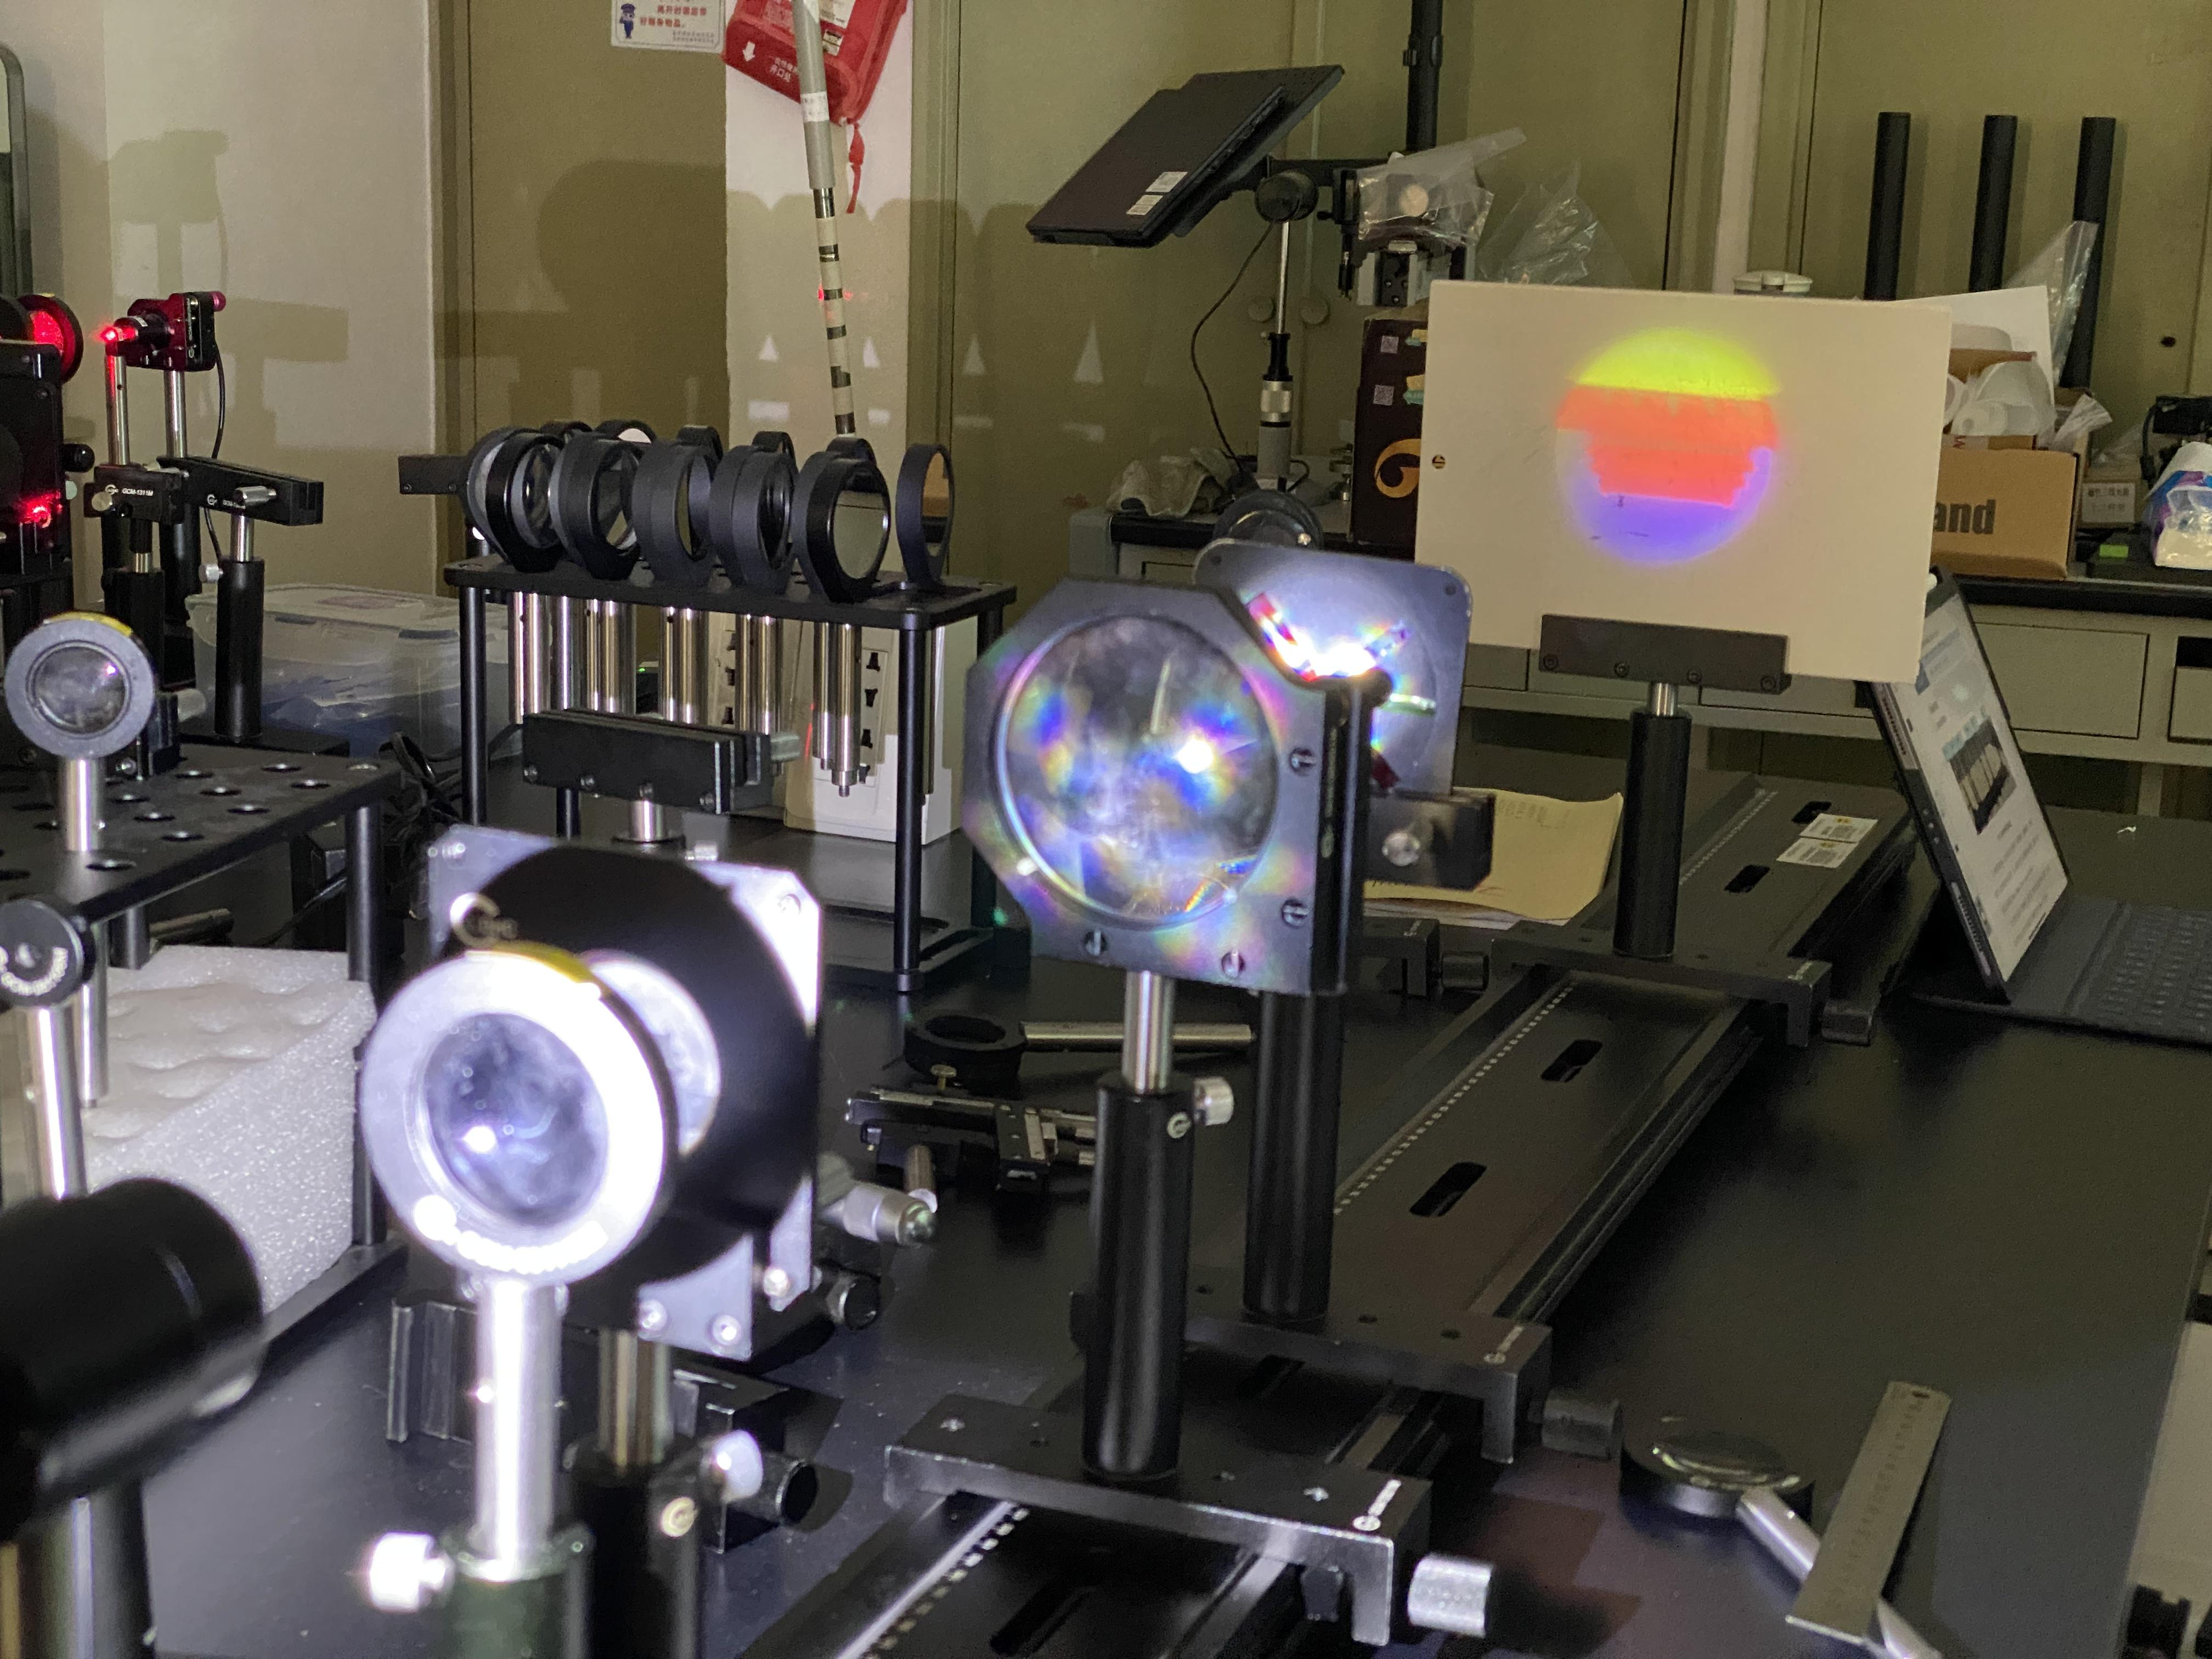
\includegraphics[height=5cm]{./pictures/photos/假彩色编码（成像效果）.jpg}
    \caption{假彩色编码（成像效果）}
    \label{fig:假彩色编码（成像效果）}
  \end{subfigure}
  \label{fig:combined}
\end{figure}

\begin{figure}[H]
  \centering
  \begin{subfigure}[b]{0.45\textwidth}
    \centering
    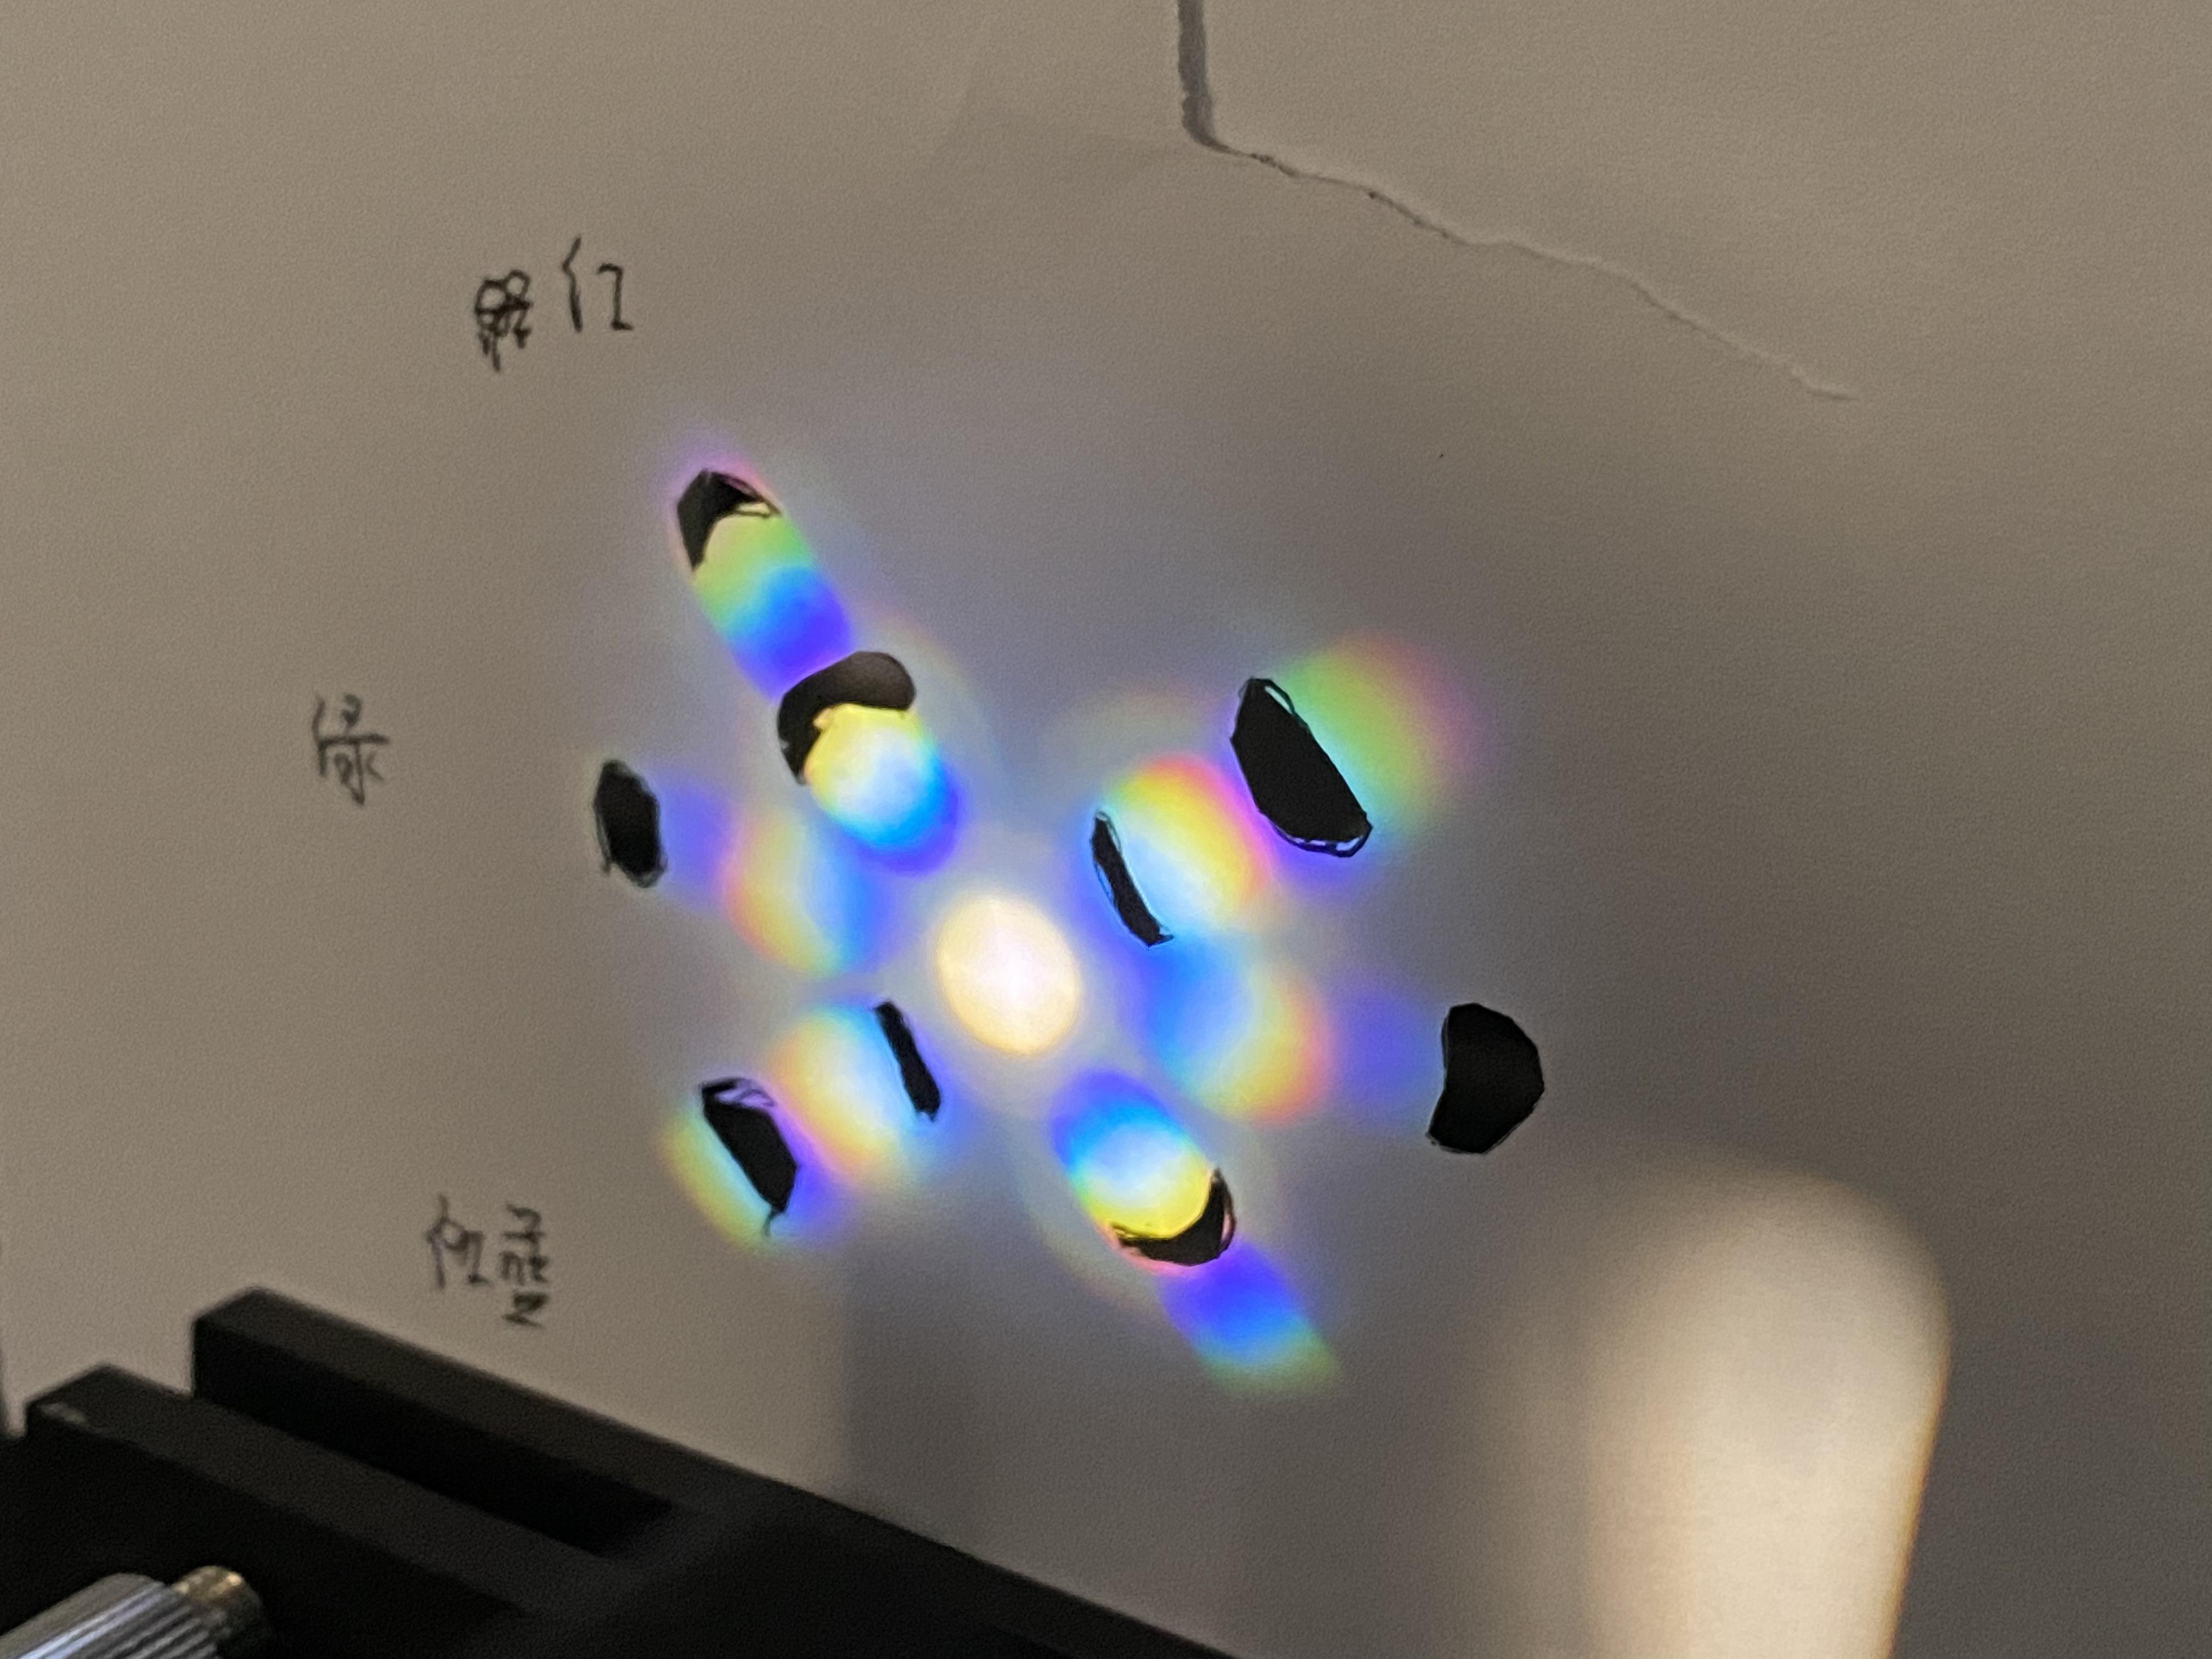
\includegraphics[height=5cm]{./pictures/photos/自制滤波器的样貌.jpg}
    \caption{自制滤波器的样貌}
    \label{fig:自制滤波器的样貌}
  \end{subfigure}
  \hfill
  \begin{subfigure}[b]{0.45\textwidth}
    \centering
    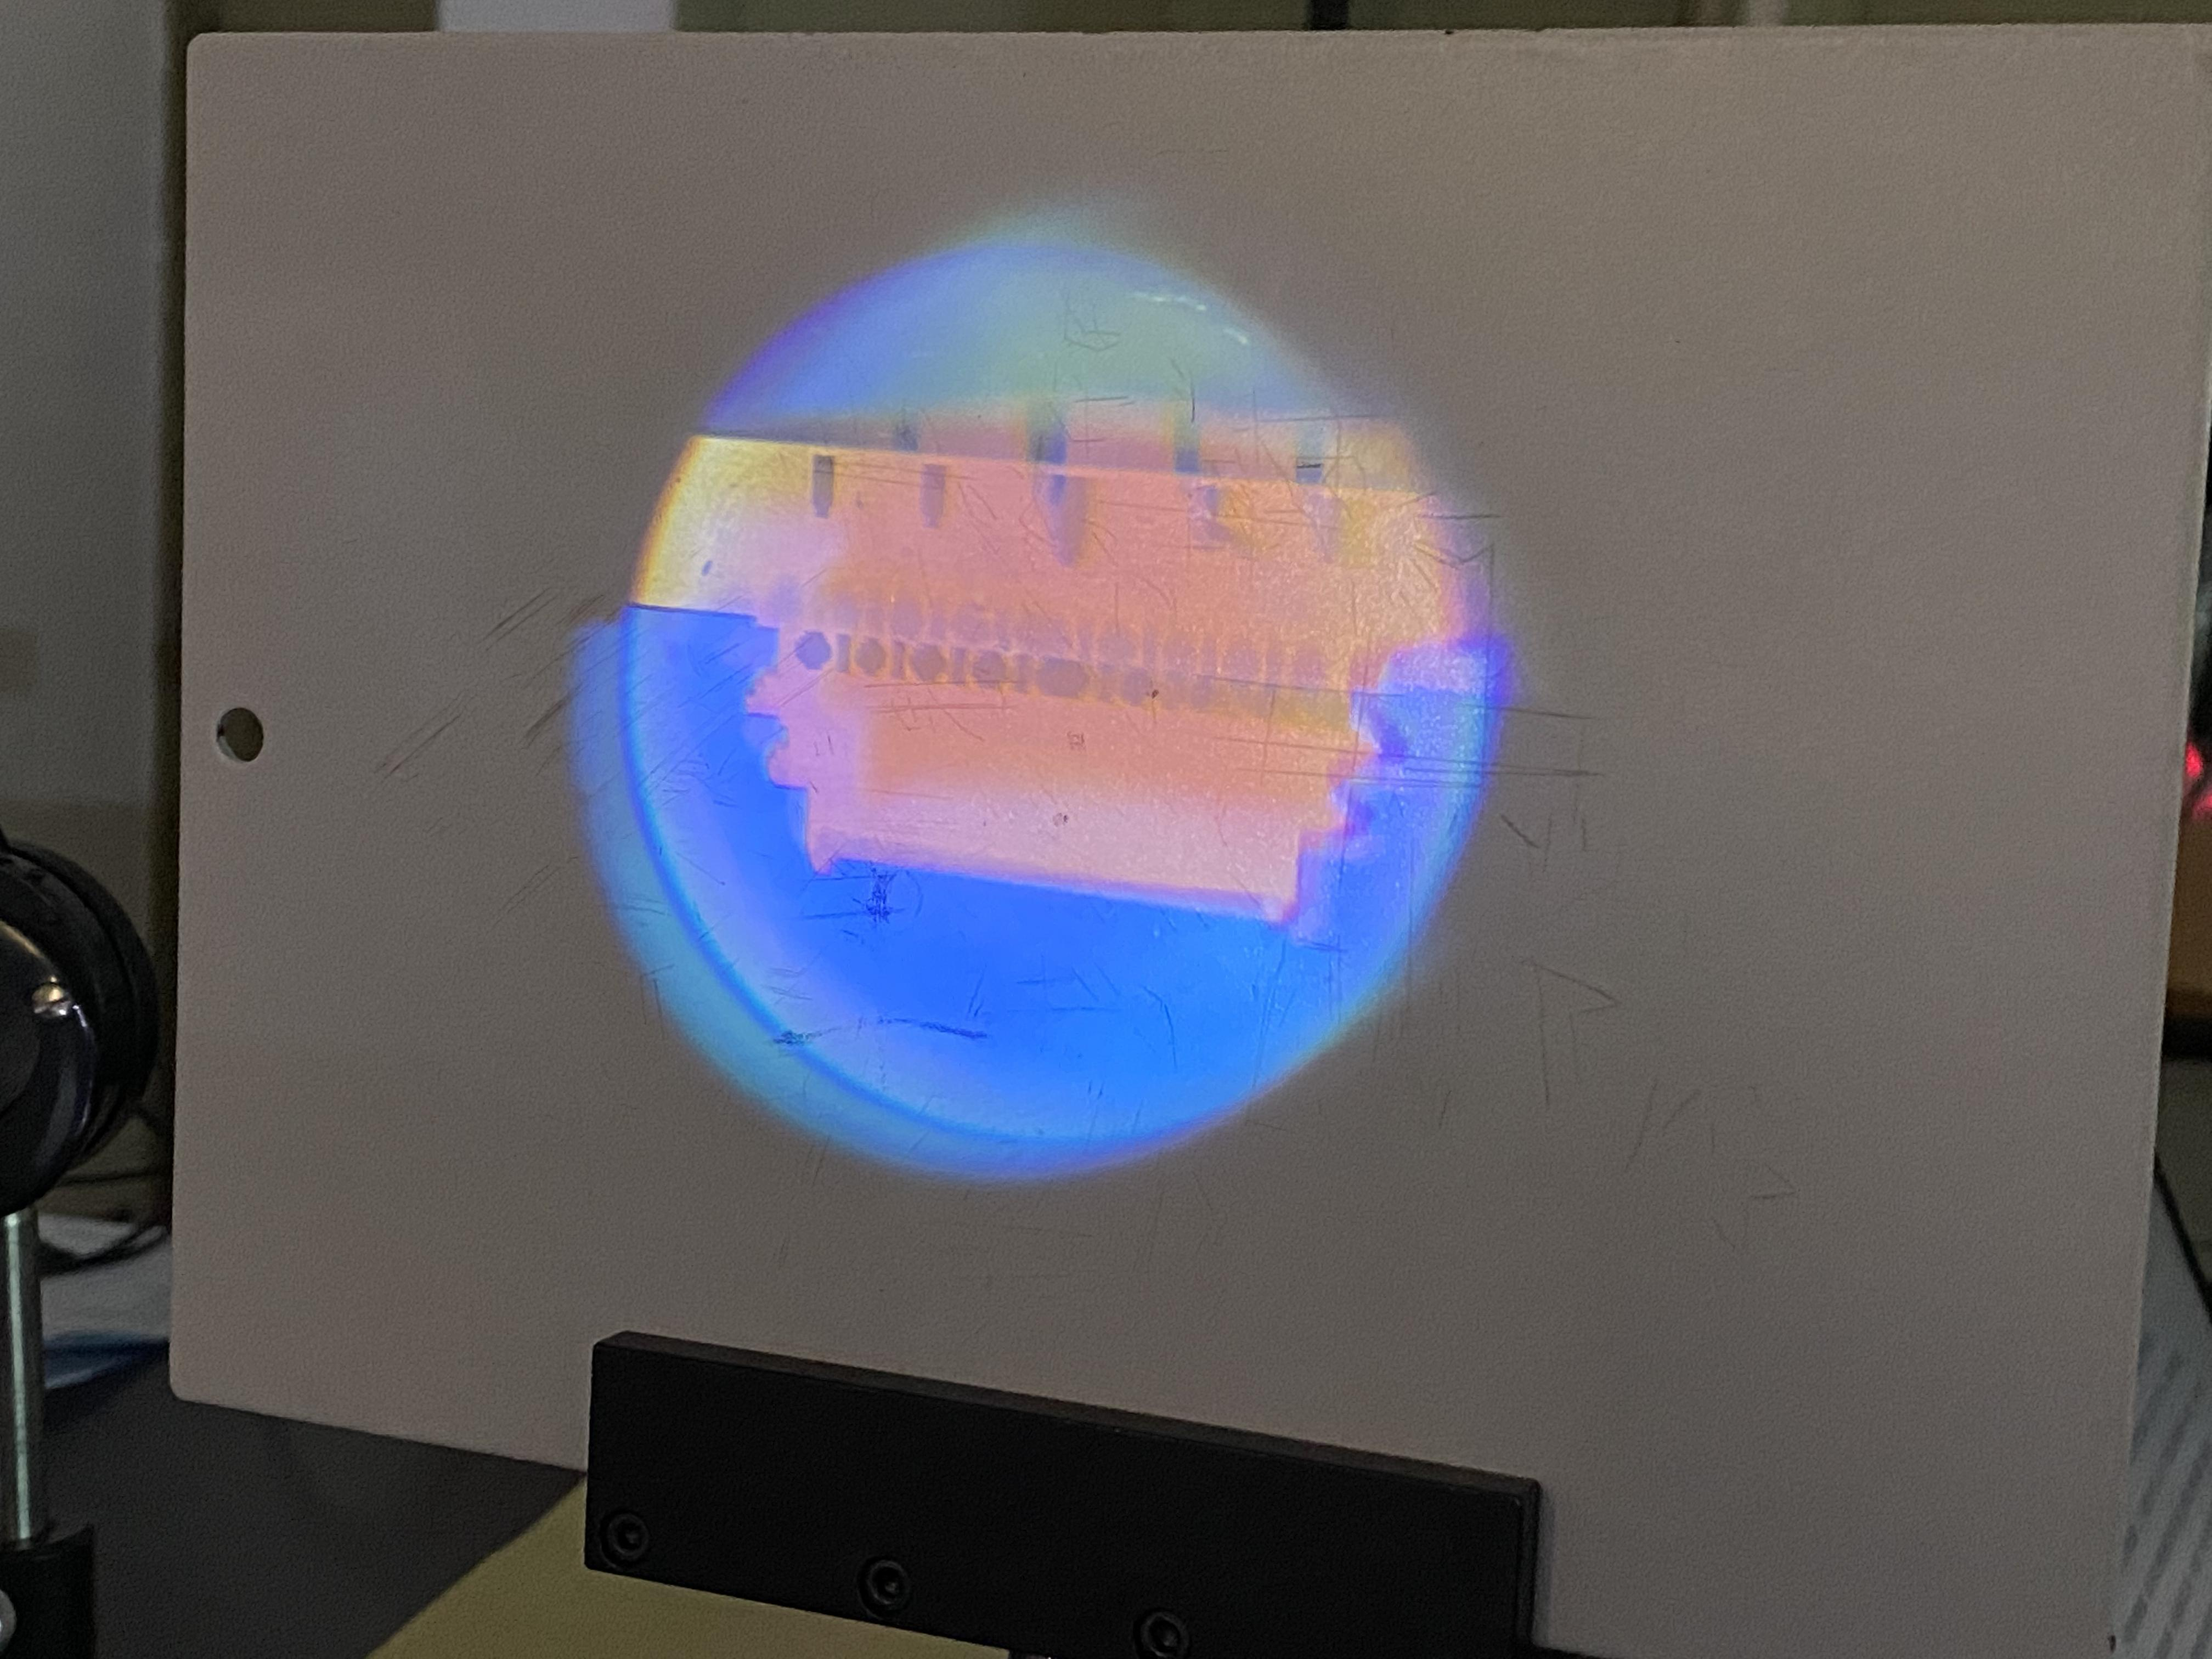
\includegraphics[height=5cm]{./pictures/photos/自制滤波器（成像效果）.jpg}
    \caption{自制滤波器（成像效果）}
    \label{fig:自制滤波器（成像效果）}
  \end{subfigure}
  \label{fig:combined}
\end{figure}


\section{衍射实验}


\subsection{实验仪器和用具}

\begin{table}[h]
\centering
\begin{tabular}{|c|c|}
\hline
\textbf{分划板 1} & \textbf{分划板 2} \\
\hline
单缝：F1: a=0.1 & 光栅：GS1: 纵横均为 50 条/毫米 \\
单缝：F2: a=0.2 & 光栅：GS2: 纵向 50 条/毫米 \\
单缝：F3: a=0.3 & 双孔（φ=0.2）：SK1: d=0.25 \\
单丝：S1: a=0.1 & 双孔（φ=0.2）：SK2: d=0.32 \\
单丝：S2: a=0.2 & 双孔（φ=0.2）：SK3: d=0.4 \\
单丝：S3: a=0.3 & 矩孔：JK: a=0.12, b=0.2 \\
小孔：XK1: φ=0.2 & 矩孔：JK: a=0.12, b=0.2 \\
小孔：XK2: φ=0.3 & 单缝：DF1: a=0.08 (右下 1) \\
小孔：XK3: φ=0.4 & 双缝：SF1: a=0.08, d=0.16 \\
& 双缝：SF2: a=0.08, d=0.20 \\
& 双缝：SF3: a=0.06, d=0.10 \\
& 多缝：DF1: 4 缝, a=0.06, d=0.1×4 \\
& 多缝：DF2: 9 缝, a=0.06, d=0.1×9 \\
\hline
\end{tabular}
\caption{分划板一和分划板二}
\label{tab:dividers}
\end{table}

\subsection{实验内容}

\begin{enumerate}
    \item \textbf{实验一：夫琅和费衍射演示实验}
    \begin{itemize}
        \item 将分划板放入光路中，观察衍射图样的变化，判断其与分划板参数的一致性。
        \item 区分缝的衍射与孔的衍射图样。
        \item 区分缝与丝、孔与屏的衍射图样。
        \item 比较单缝、双缝与多缝的衍射图样。
        \item 判断单缝与多缝的衍射效果。
        \item 区分一维光栅和二维光栅的衍射图样。
    \end{itemize}

    \item \textbf{实验二：光栅衍射测量光栅常数实验}
    \begin{itemize}
        \item 将透射光栅放入光路中，观察衍射光斑图样，利用光栅方程计算光栅常数 \(d\)，并判断与已知光栅刻缝数的一致性。
        \item 光栅方程为：
        \[
        d \sin \theta_m = m \lambda \quad (m = 0, \pm 1, \pm 2, \ldots)
        \]
        其中，\(d\) 为相邻两缝的中心距离，\(\theta\) 为从干涉图样中心到第 \(m\) 级极大之间的夹角，\(\lambda\) 为光的波长，\(m\) 为级次。
    \end{itemize}

    \item \textbf{实验三：光栅光谱仪测光谱实验}
    \begin{itemize}
        \item 使用手持式光栅光谱仪和 SpectraSmart 软件测量白光或单色光光谱，记录中心波长、峰值强度与线宽，并判断与经验值的一致性。
    \end{itemize}
\end{enumerate}

\subsection{实验效果}

\subsubsection{实验一：夫琅和费衍射演示实验}
\begin{figure}[H]
  \centering
  \begin{subfigure}[b]{0.45\textwidth}
    \centering
    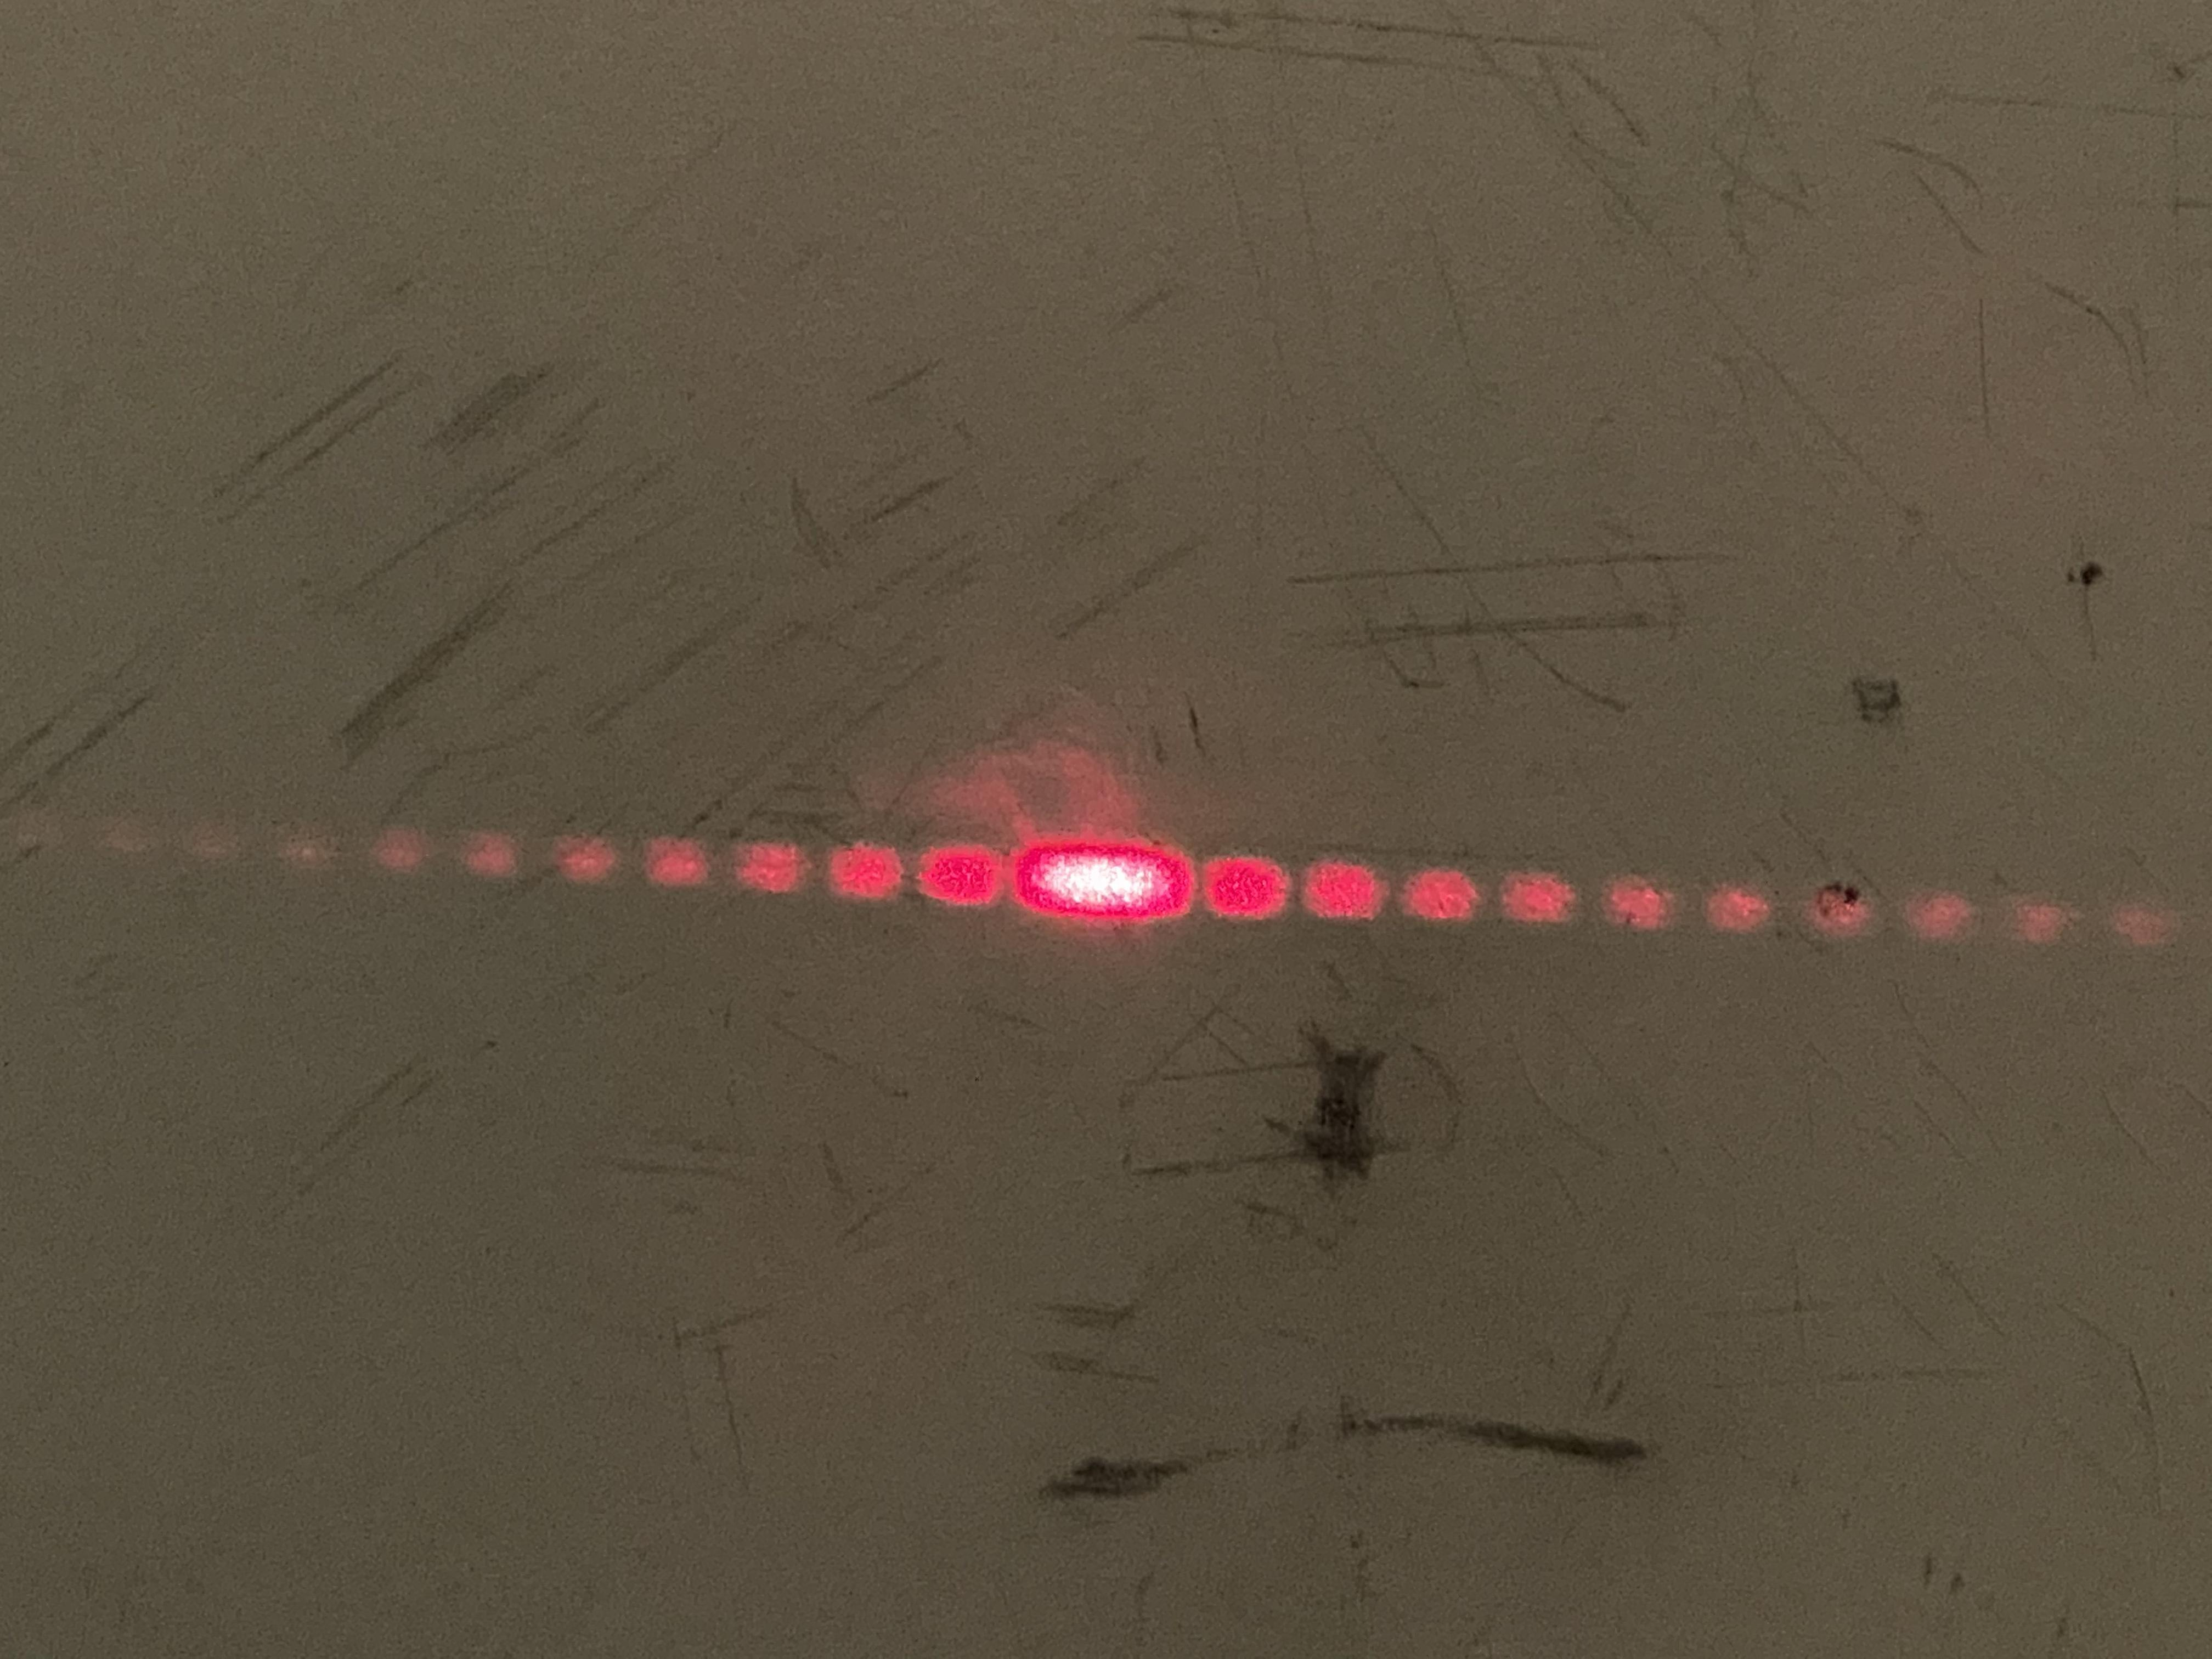
\includegraphics[height=5cm]{./pictures/photos/分划板1_单缝1.jpg}
    \caption{分划板1 单缝1}
    \label{fig:分划板1_单缝1}
  \end{subfigure}
  \hfill
  \begin{subfigure}[b]{0.45\textwidth}
    \centering
    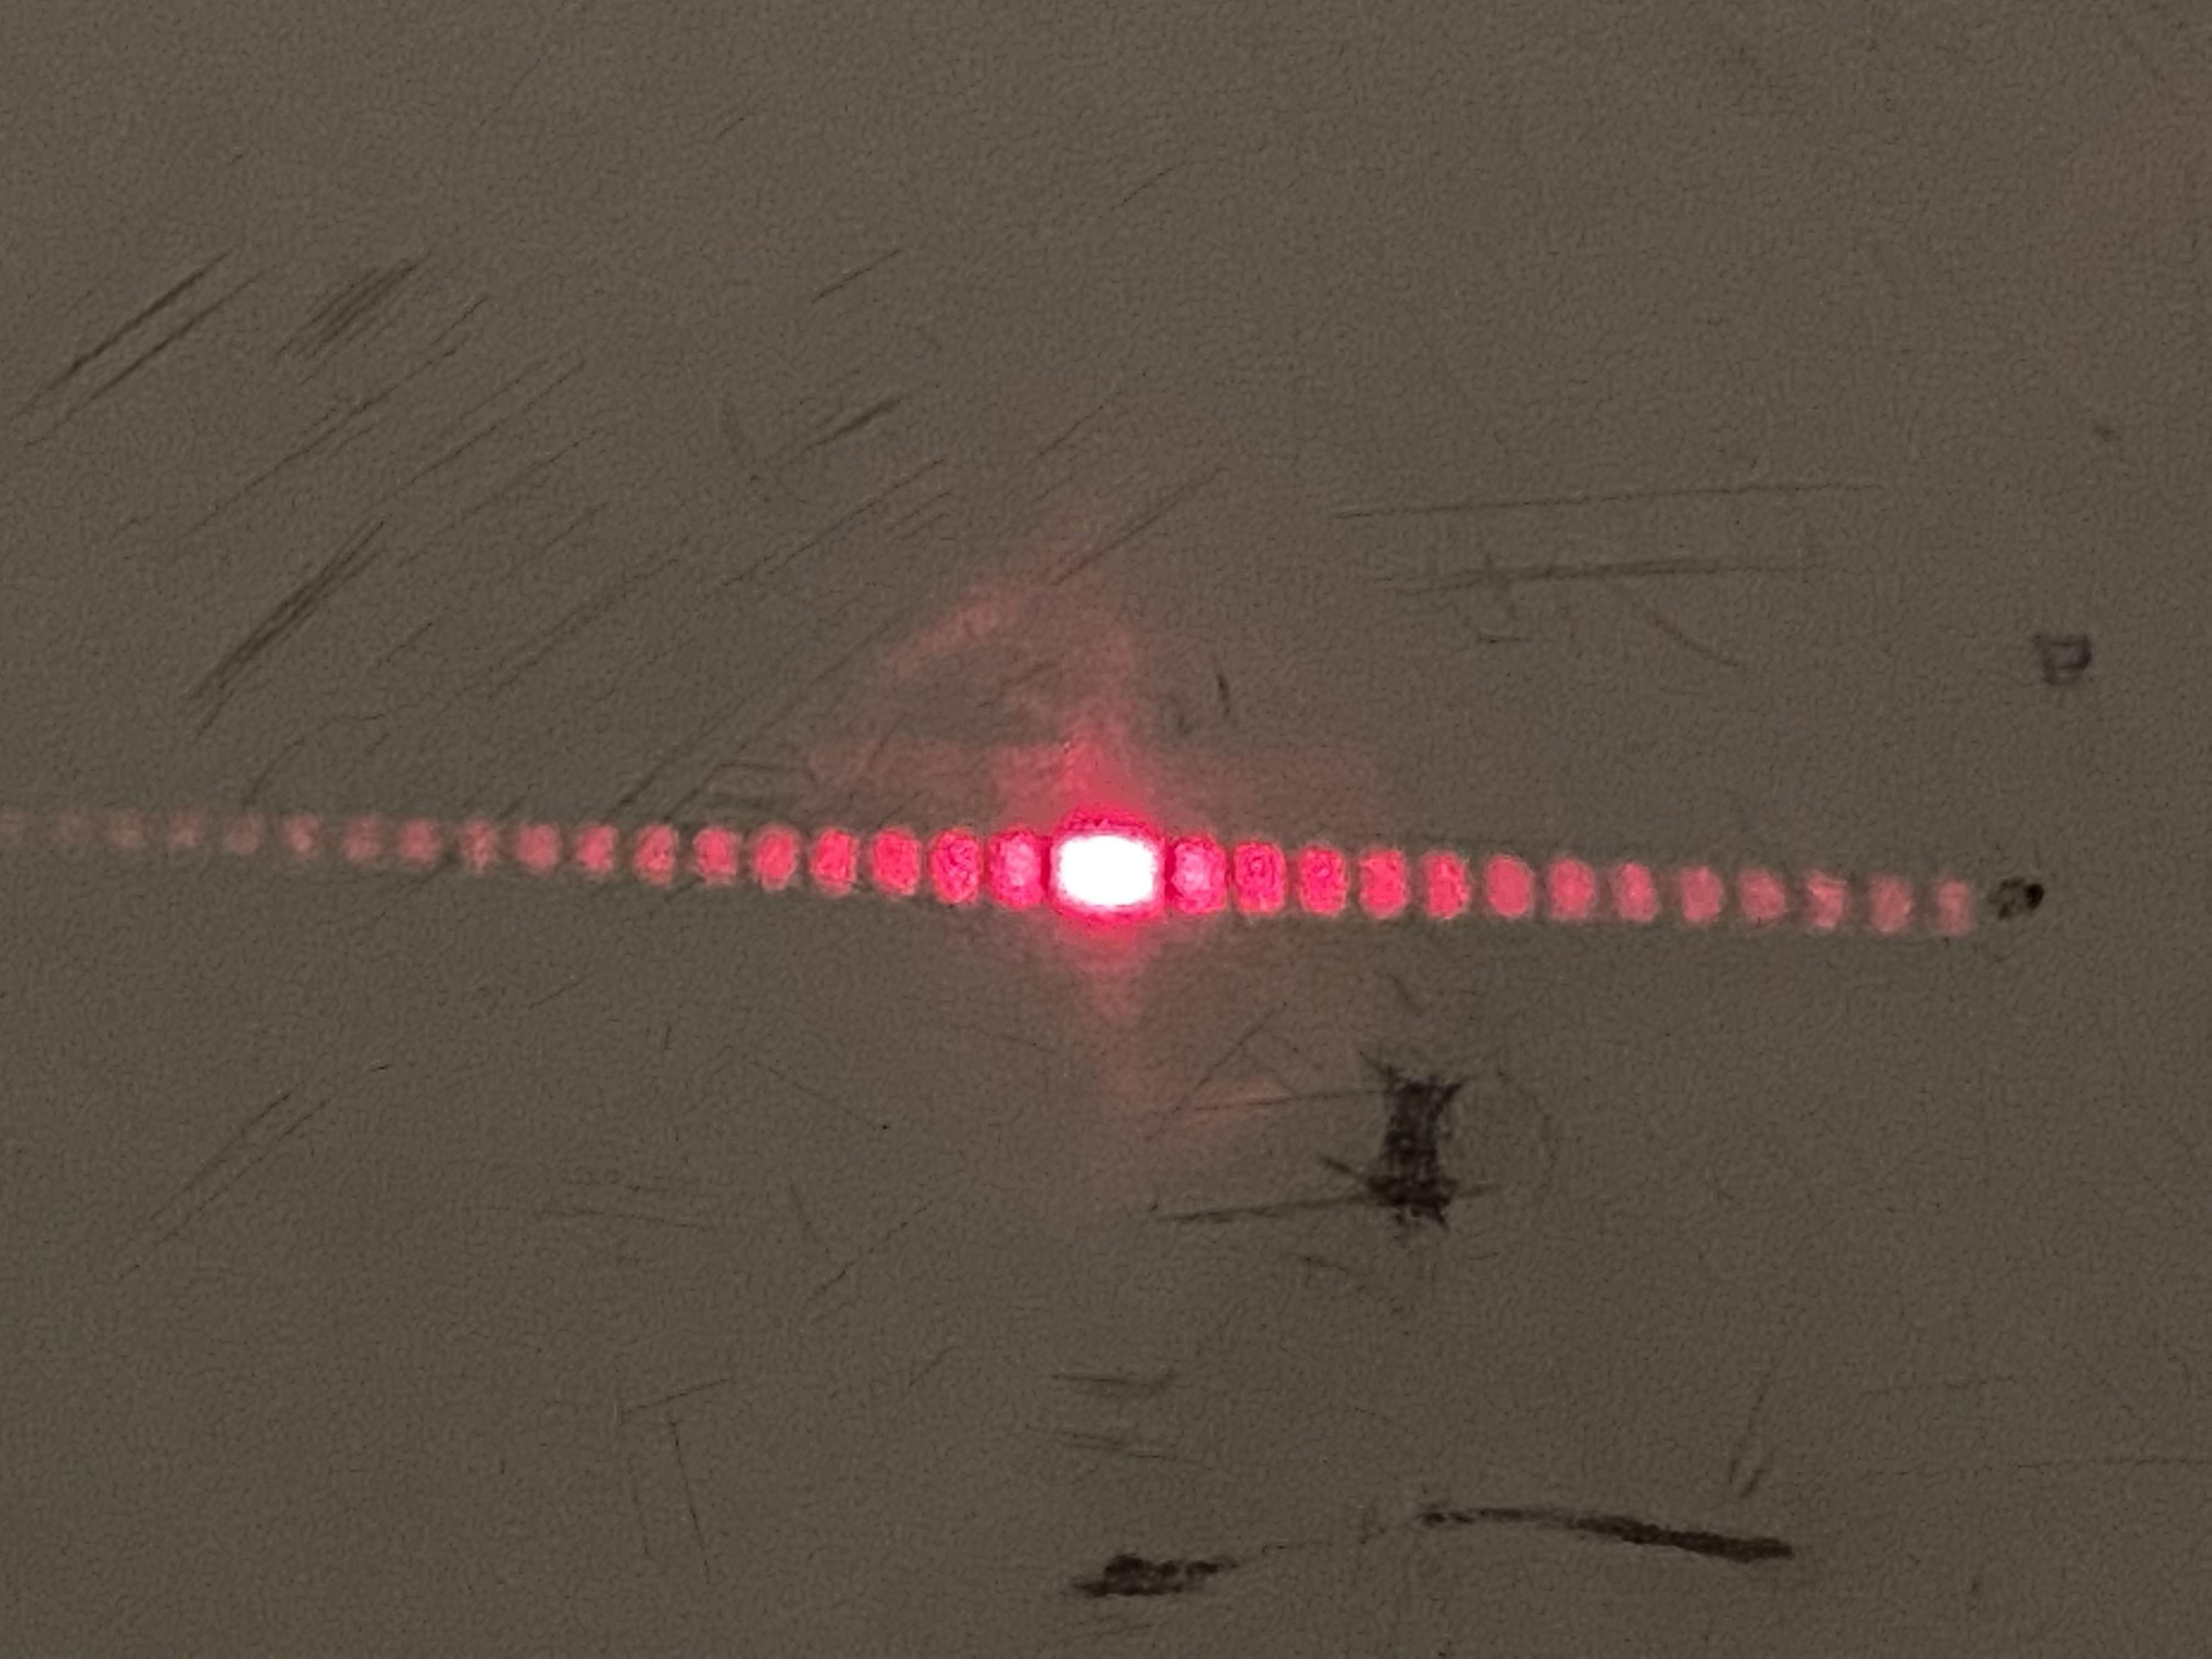
\includegraphics[height=5cm]{./pictures/photos/分划板1_单缝2.jpg}
    \caption{分划板1 单缝2}
    \label{fig:分划板1_单缝2}
  \end{subfigure}
  \label{fig:combined}
\end{figure}

\begin{figure}[H]
  \centering
  \begin{subfigure}[b]{0.45\textwidth}
    \centering
    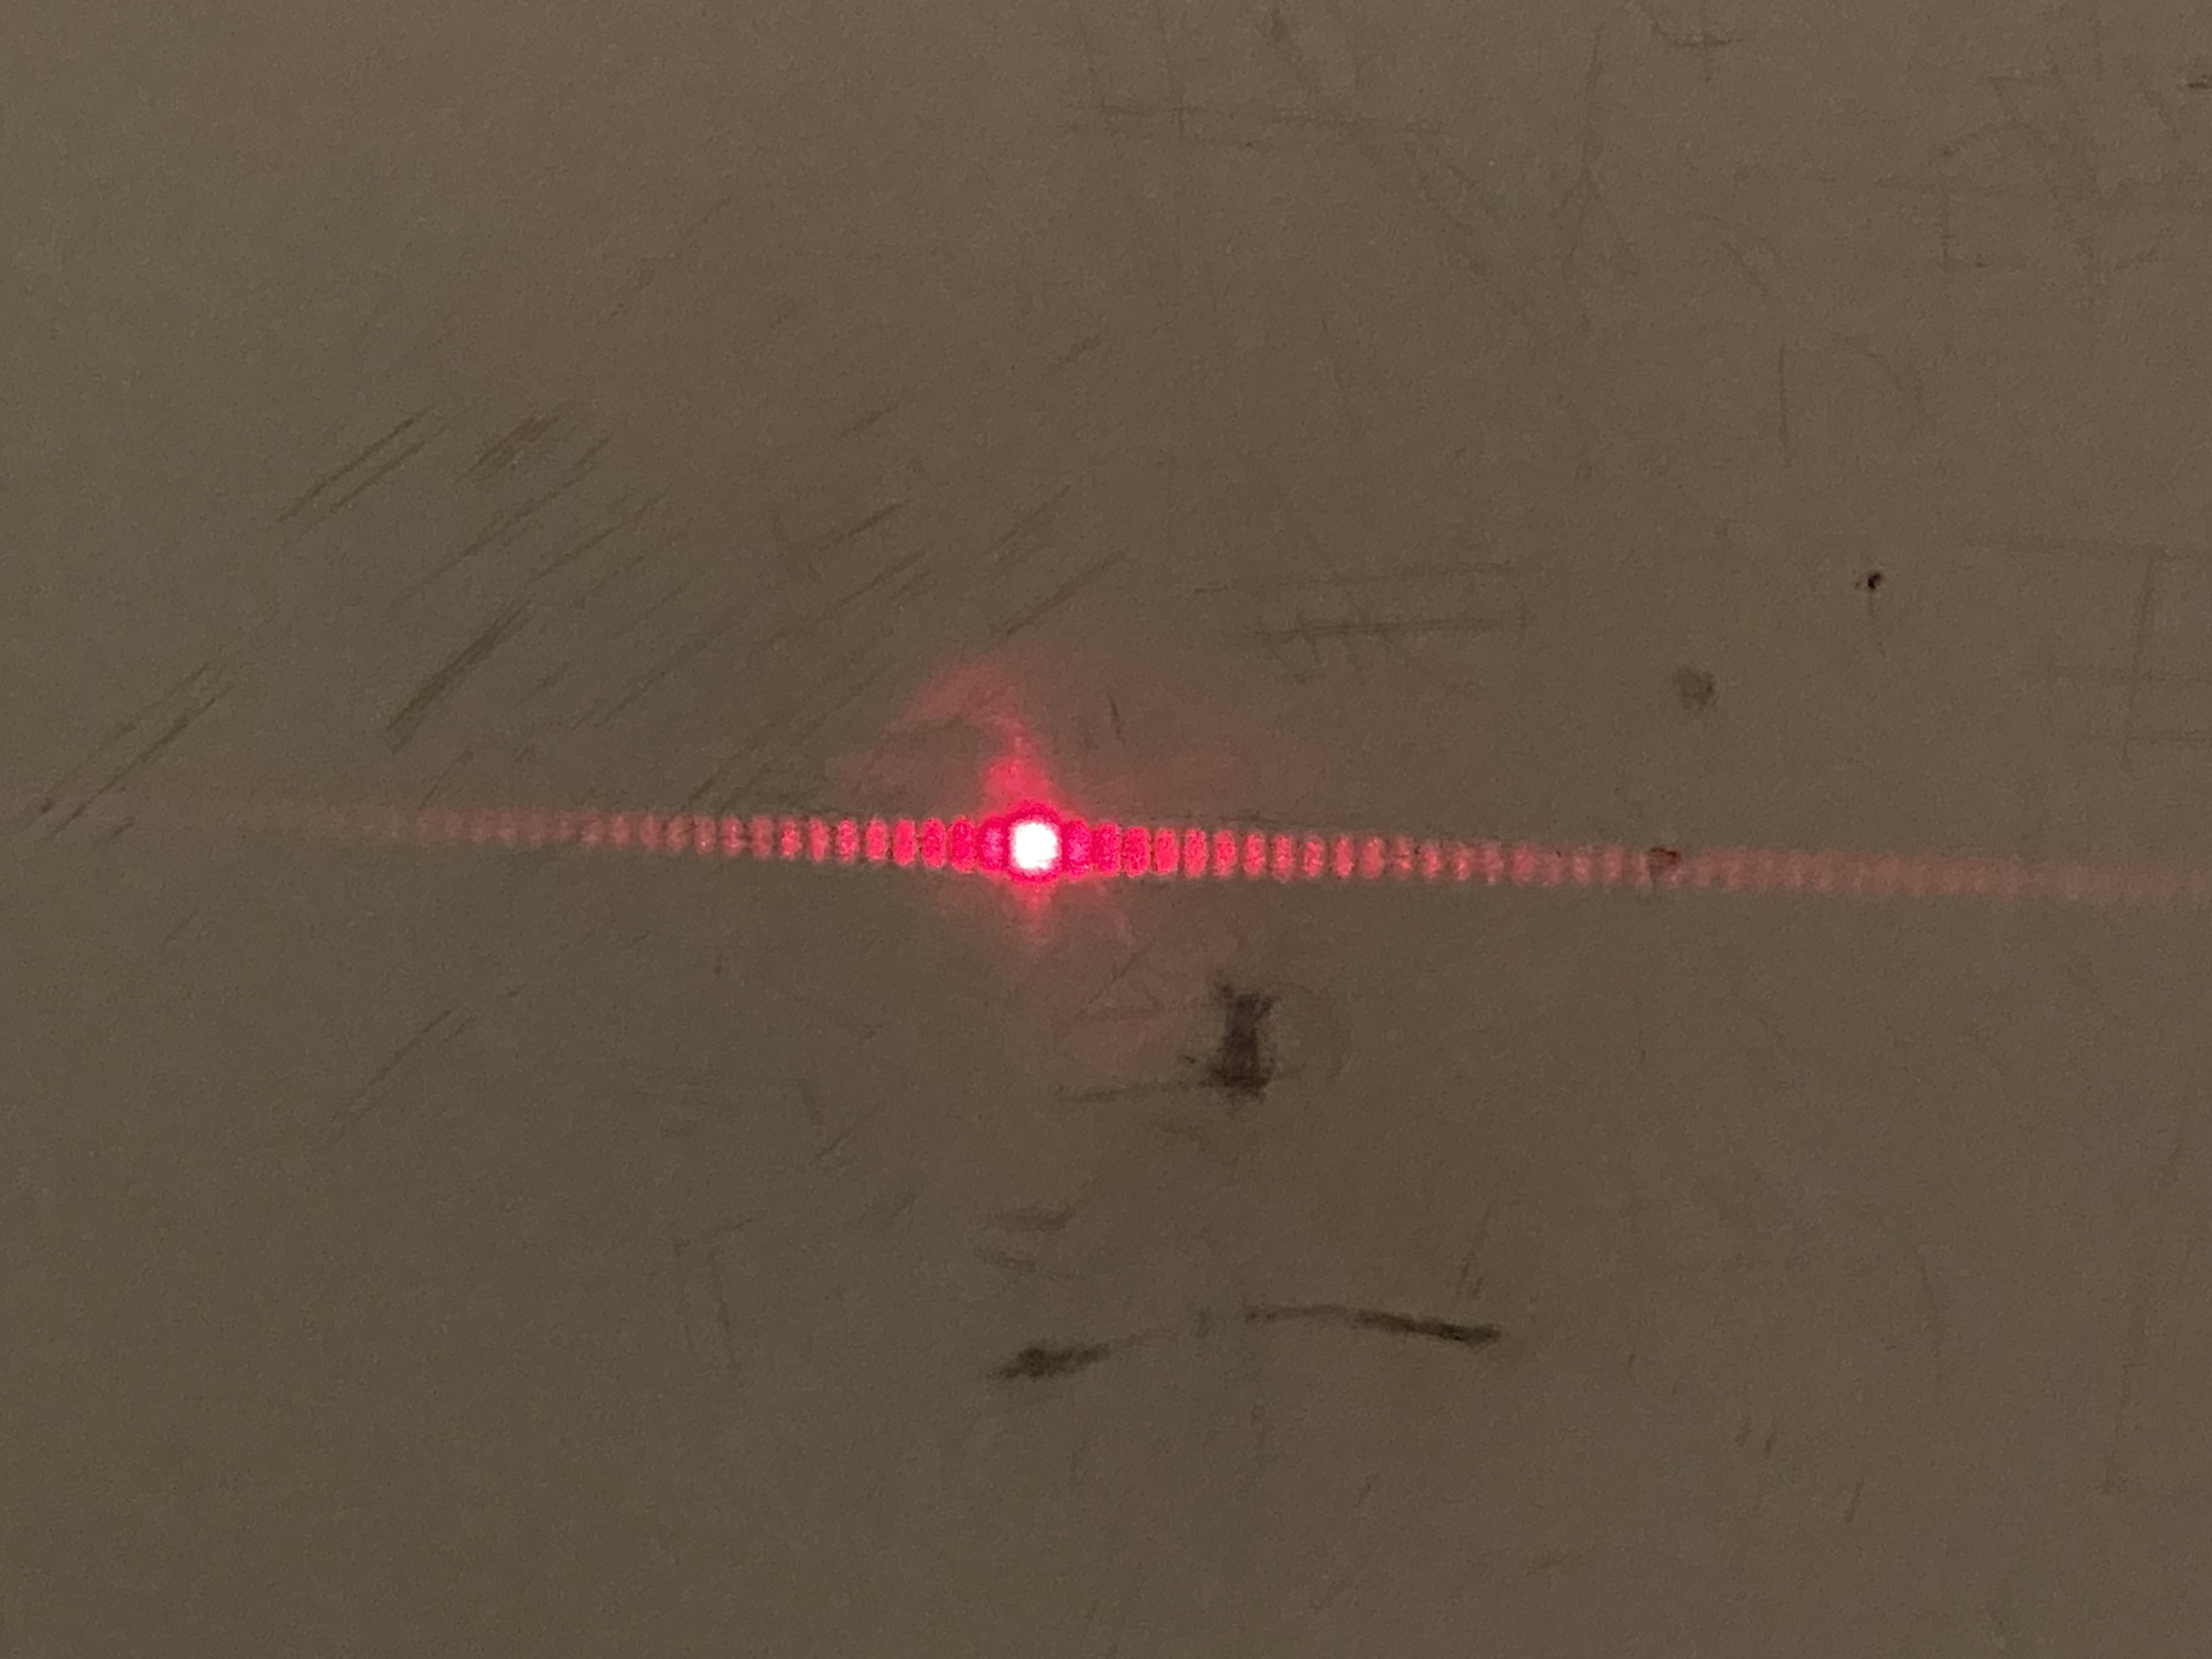
\includegraphics[height=5cm]{./pictures/photos/分划板1_单缝3.jpg}
    \caption{分划板1 单缝3}
    \label{fig:分划板1_单缝3}
  \end{subfigure}
  \hfill
  \begin{subfigure}[b]{0.45\textwidth}
    \centering
    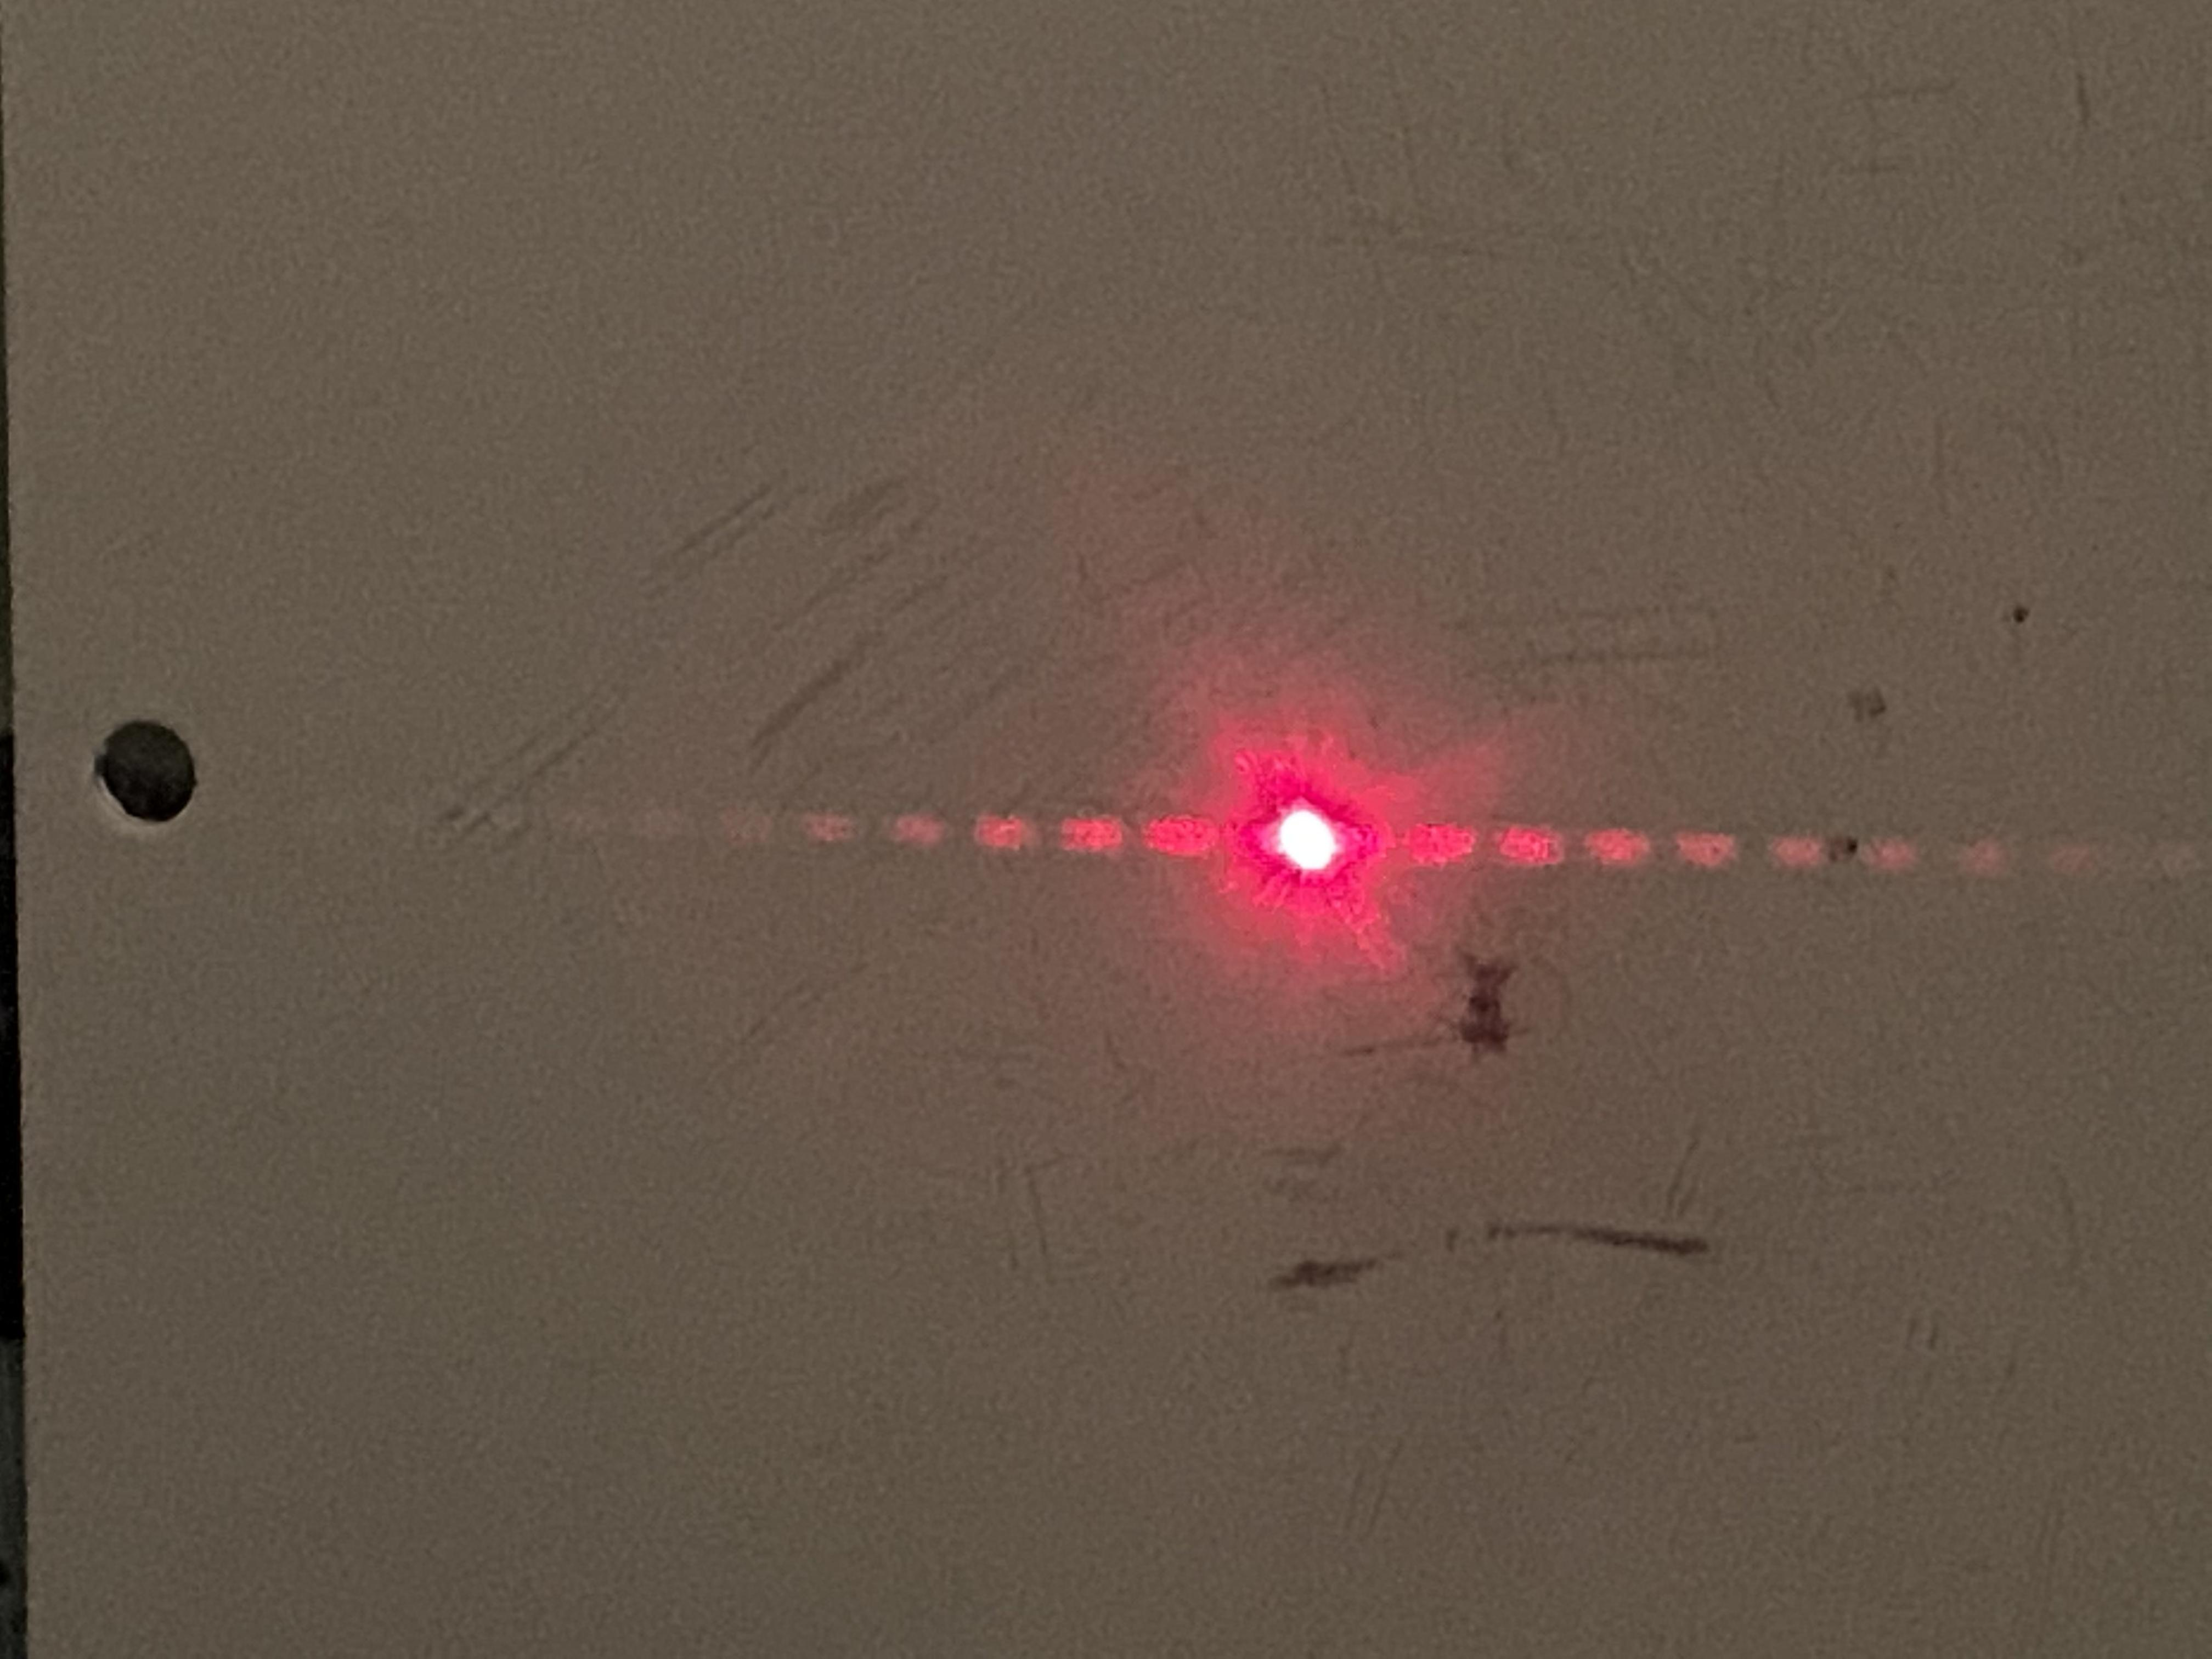
\includegraphics[height=5cm]{./pictures/photos/分划板1_单丝1.jpg}
    \caption{分划板1 单丝1}
    \label{fig:分划板1_单丝1}
  \end{subfigure}
  \label{fig:combined}
\end{figure}

\begin{figure}[H]
  \centering
  \begin{subfigure}[b]{0.45\textwidth}
    \centering
    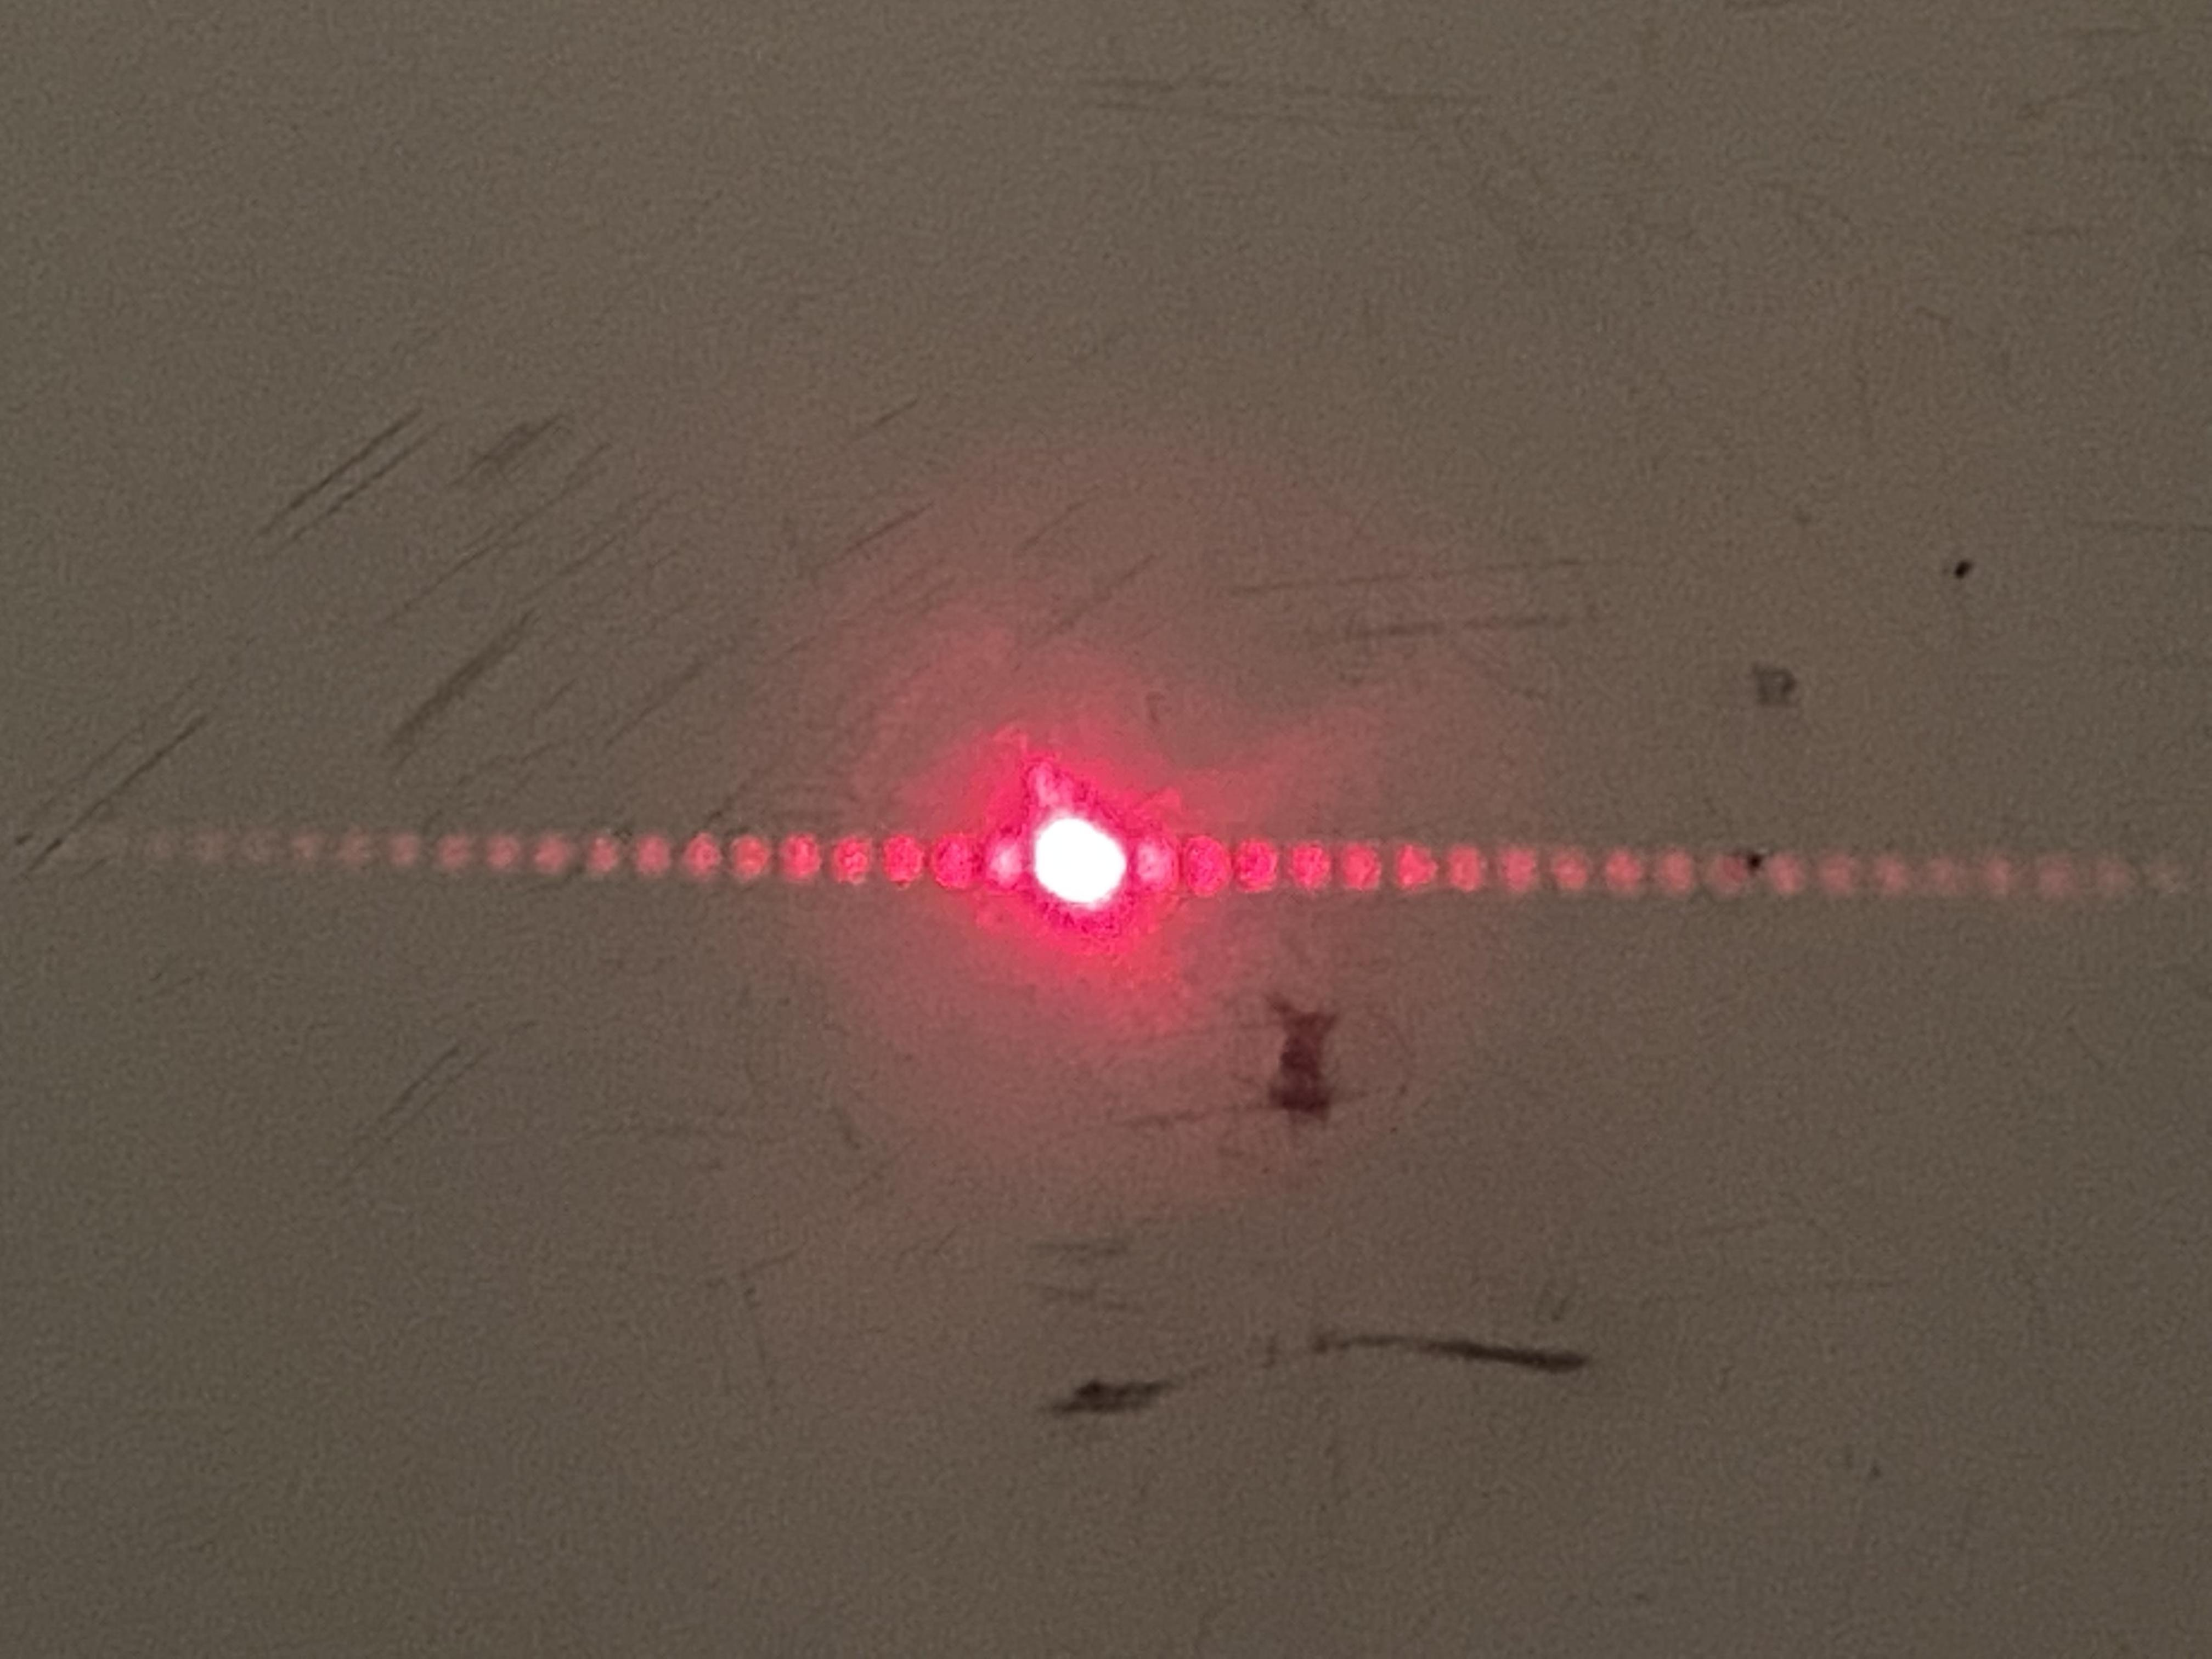
\includegraphics[height=5cm]{./pictures/photos/分划板1_单丝2.jpg}
    \caption{分划板1 单丝2}
    \label{fig:分划板1_单丝2}
  \end{subfigure}
  \hfill
  \begin{subfigure}[b]{0.45\textwidth}
    \centering
    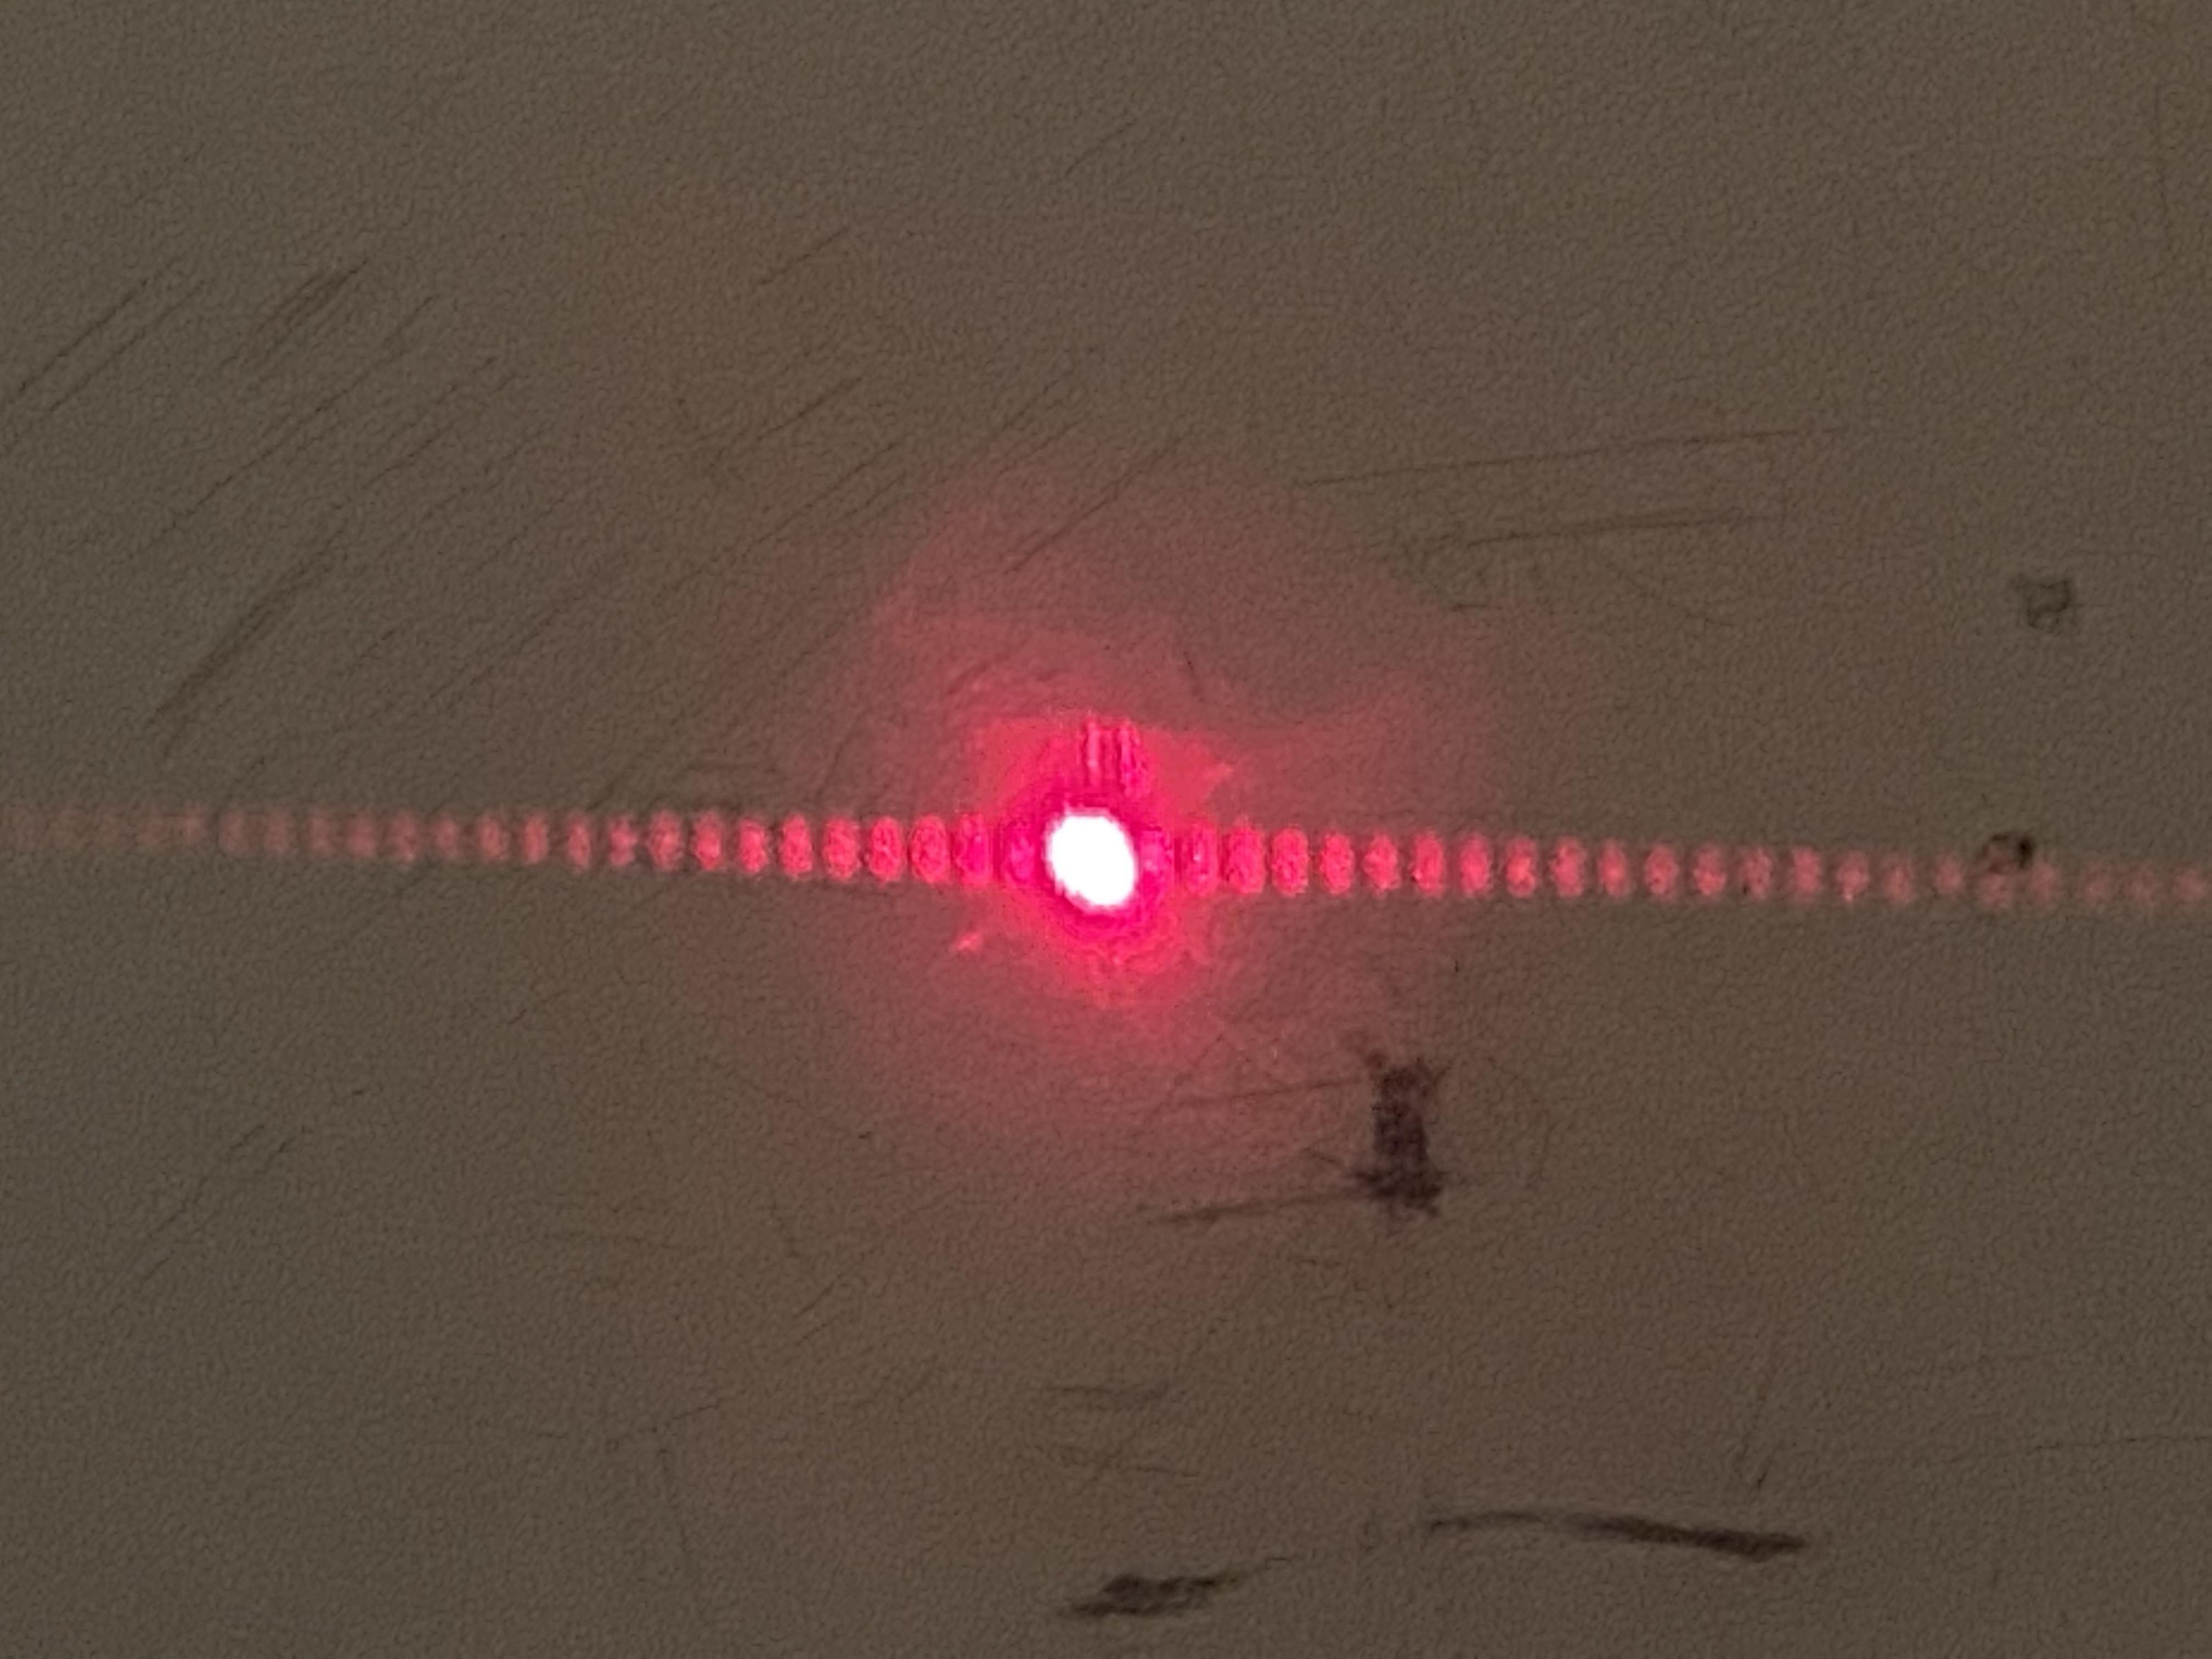
\includegraphics[height=5cm]{./pictures/photos/分划板1_单丝3.jpg}
    \caption{分划板1 单丝3}
    \label{fig:分划板1_单丝3}
  \end{subfigure}
  \label{fig:combined}
\end{figure}

\begin{figure}[H]
  \centering
  \begin{subfigure}[b]{0.45\textwidth}
    \centering
    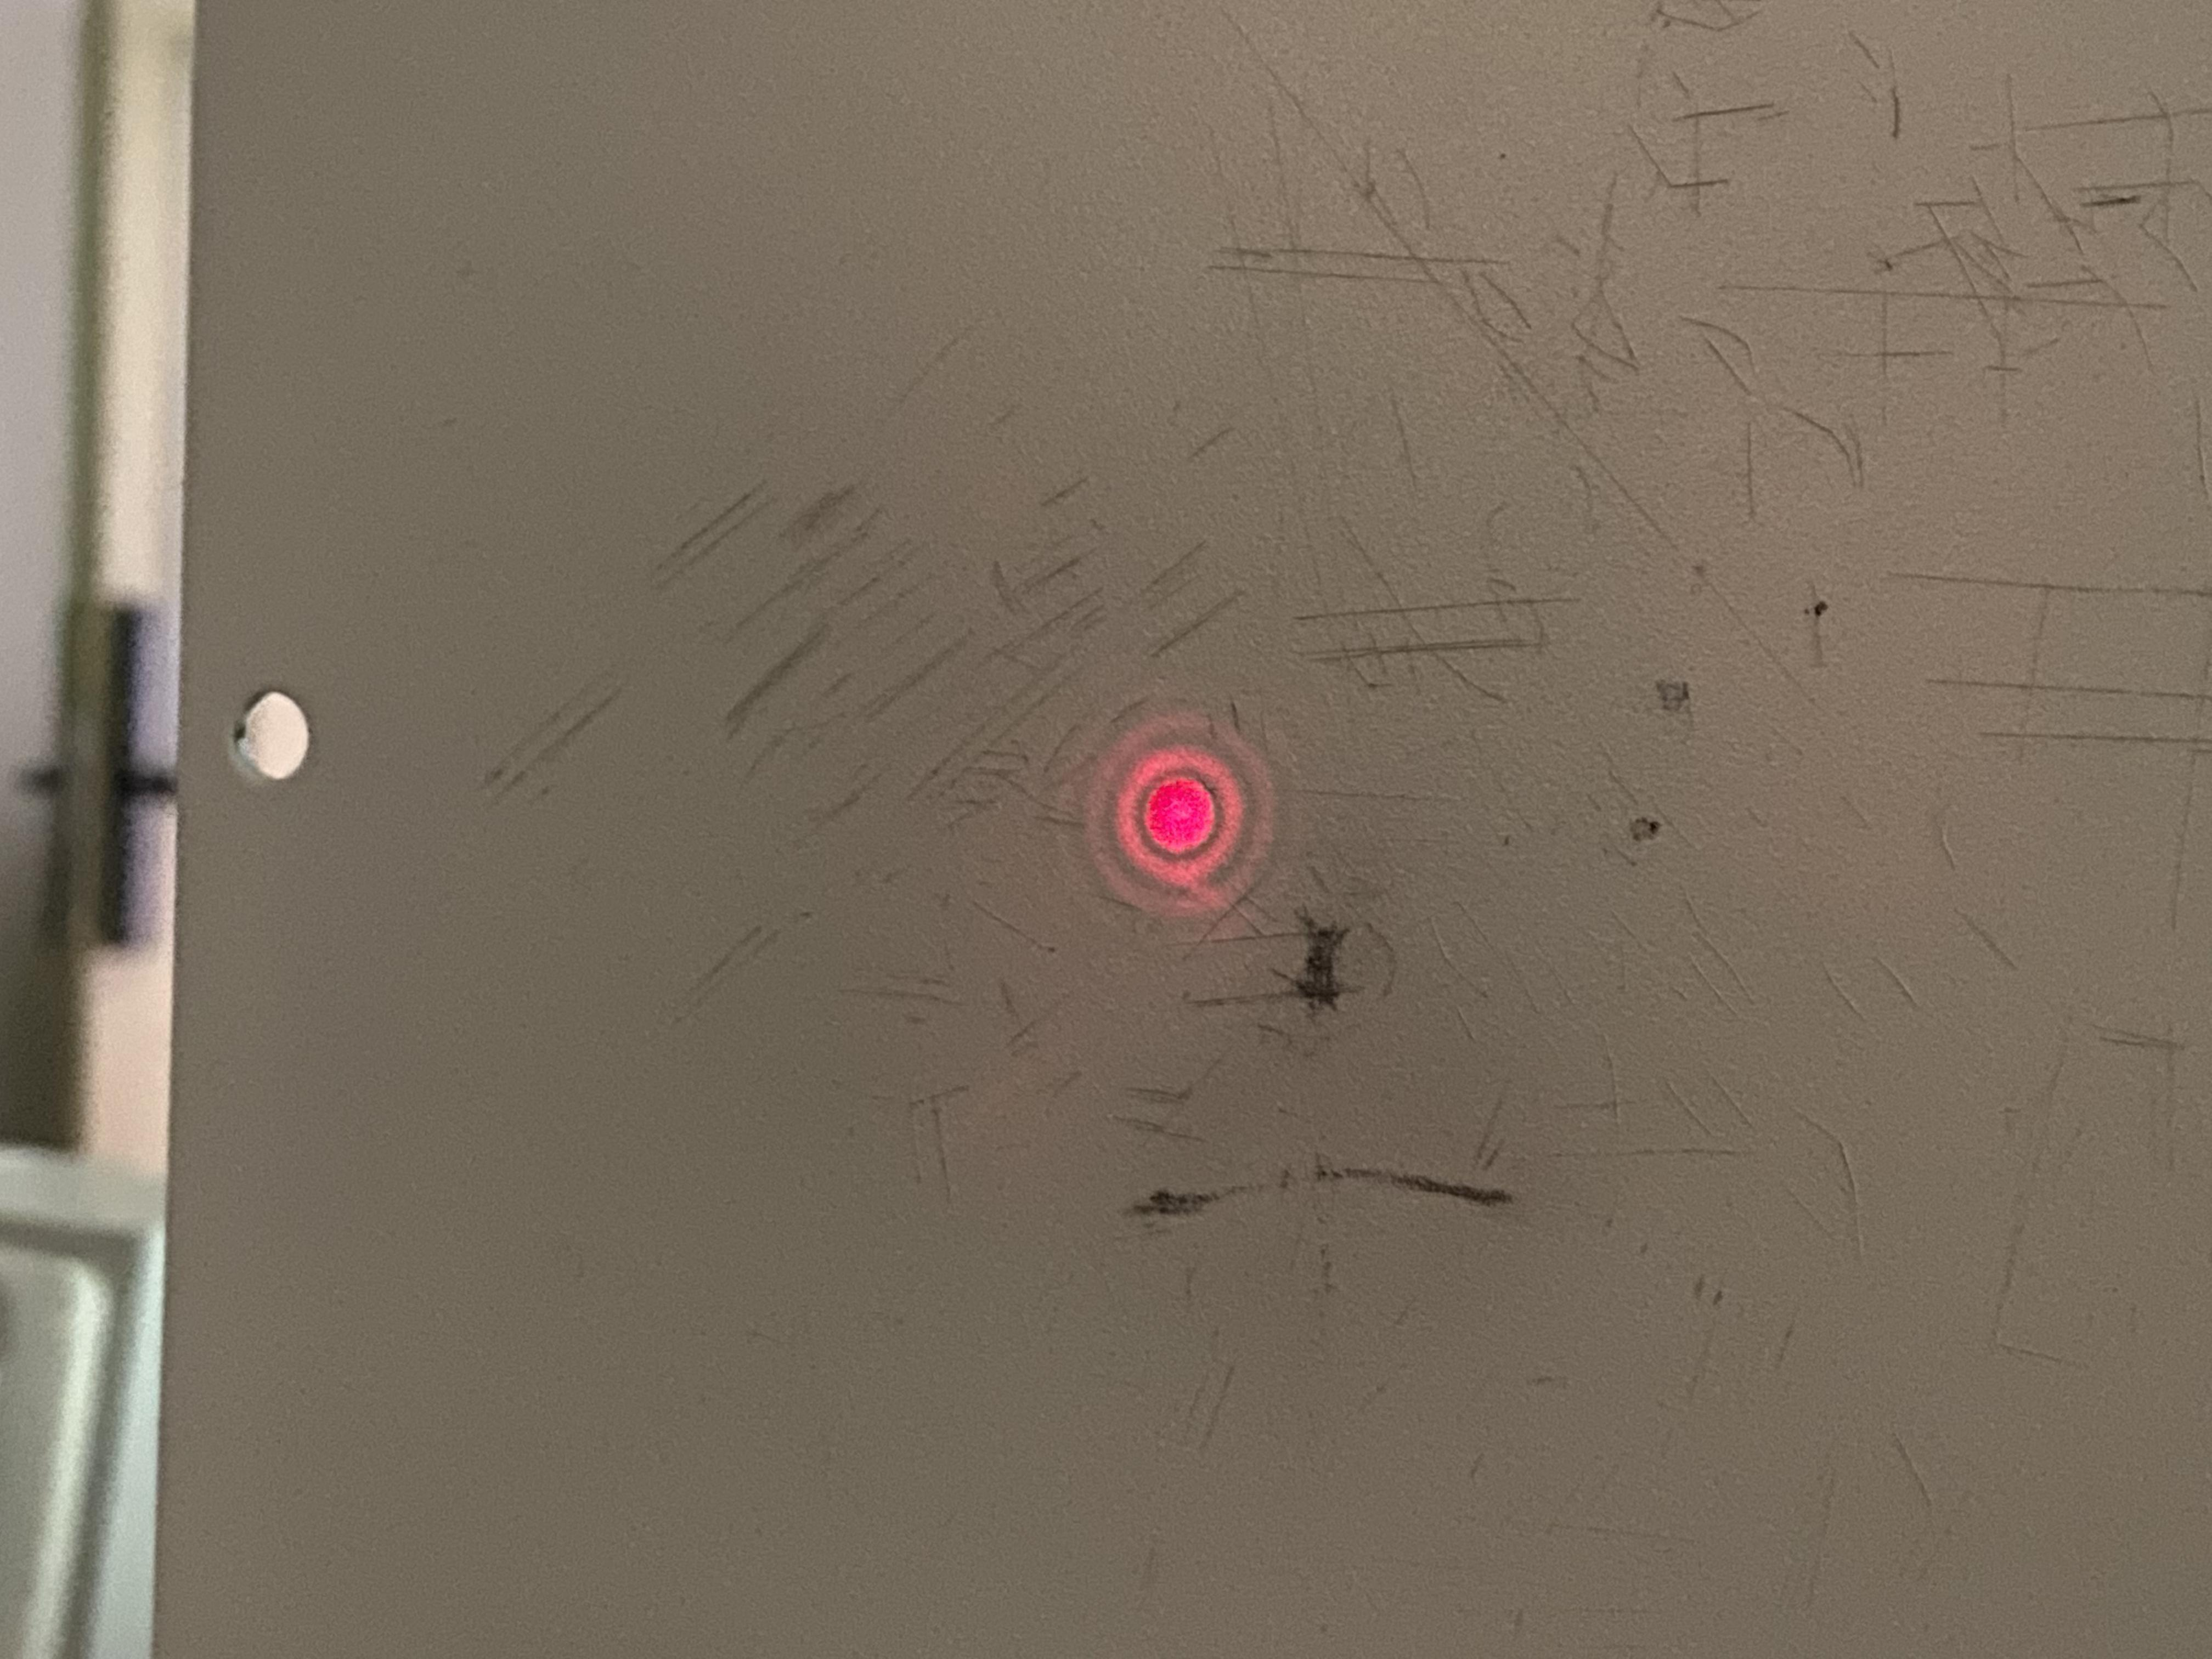
\includegraphics[height=5cm]{./pictures/photos/分划板1_小孔1.jpg}
    \caption{分划板1 小孔1}
    \label{fig:分划板1_小孔1}
  \end{subfigure}
  \hfill
  \begin{subfigure}[b]{0.45\textwidth}
    \centering
    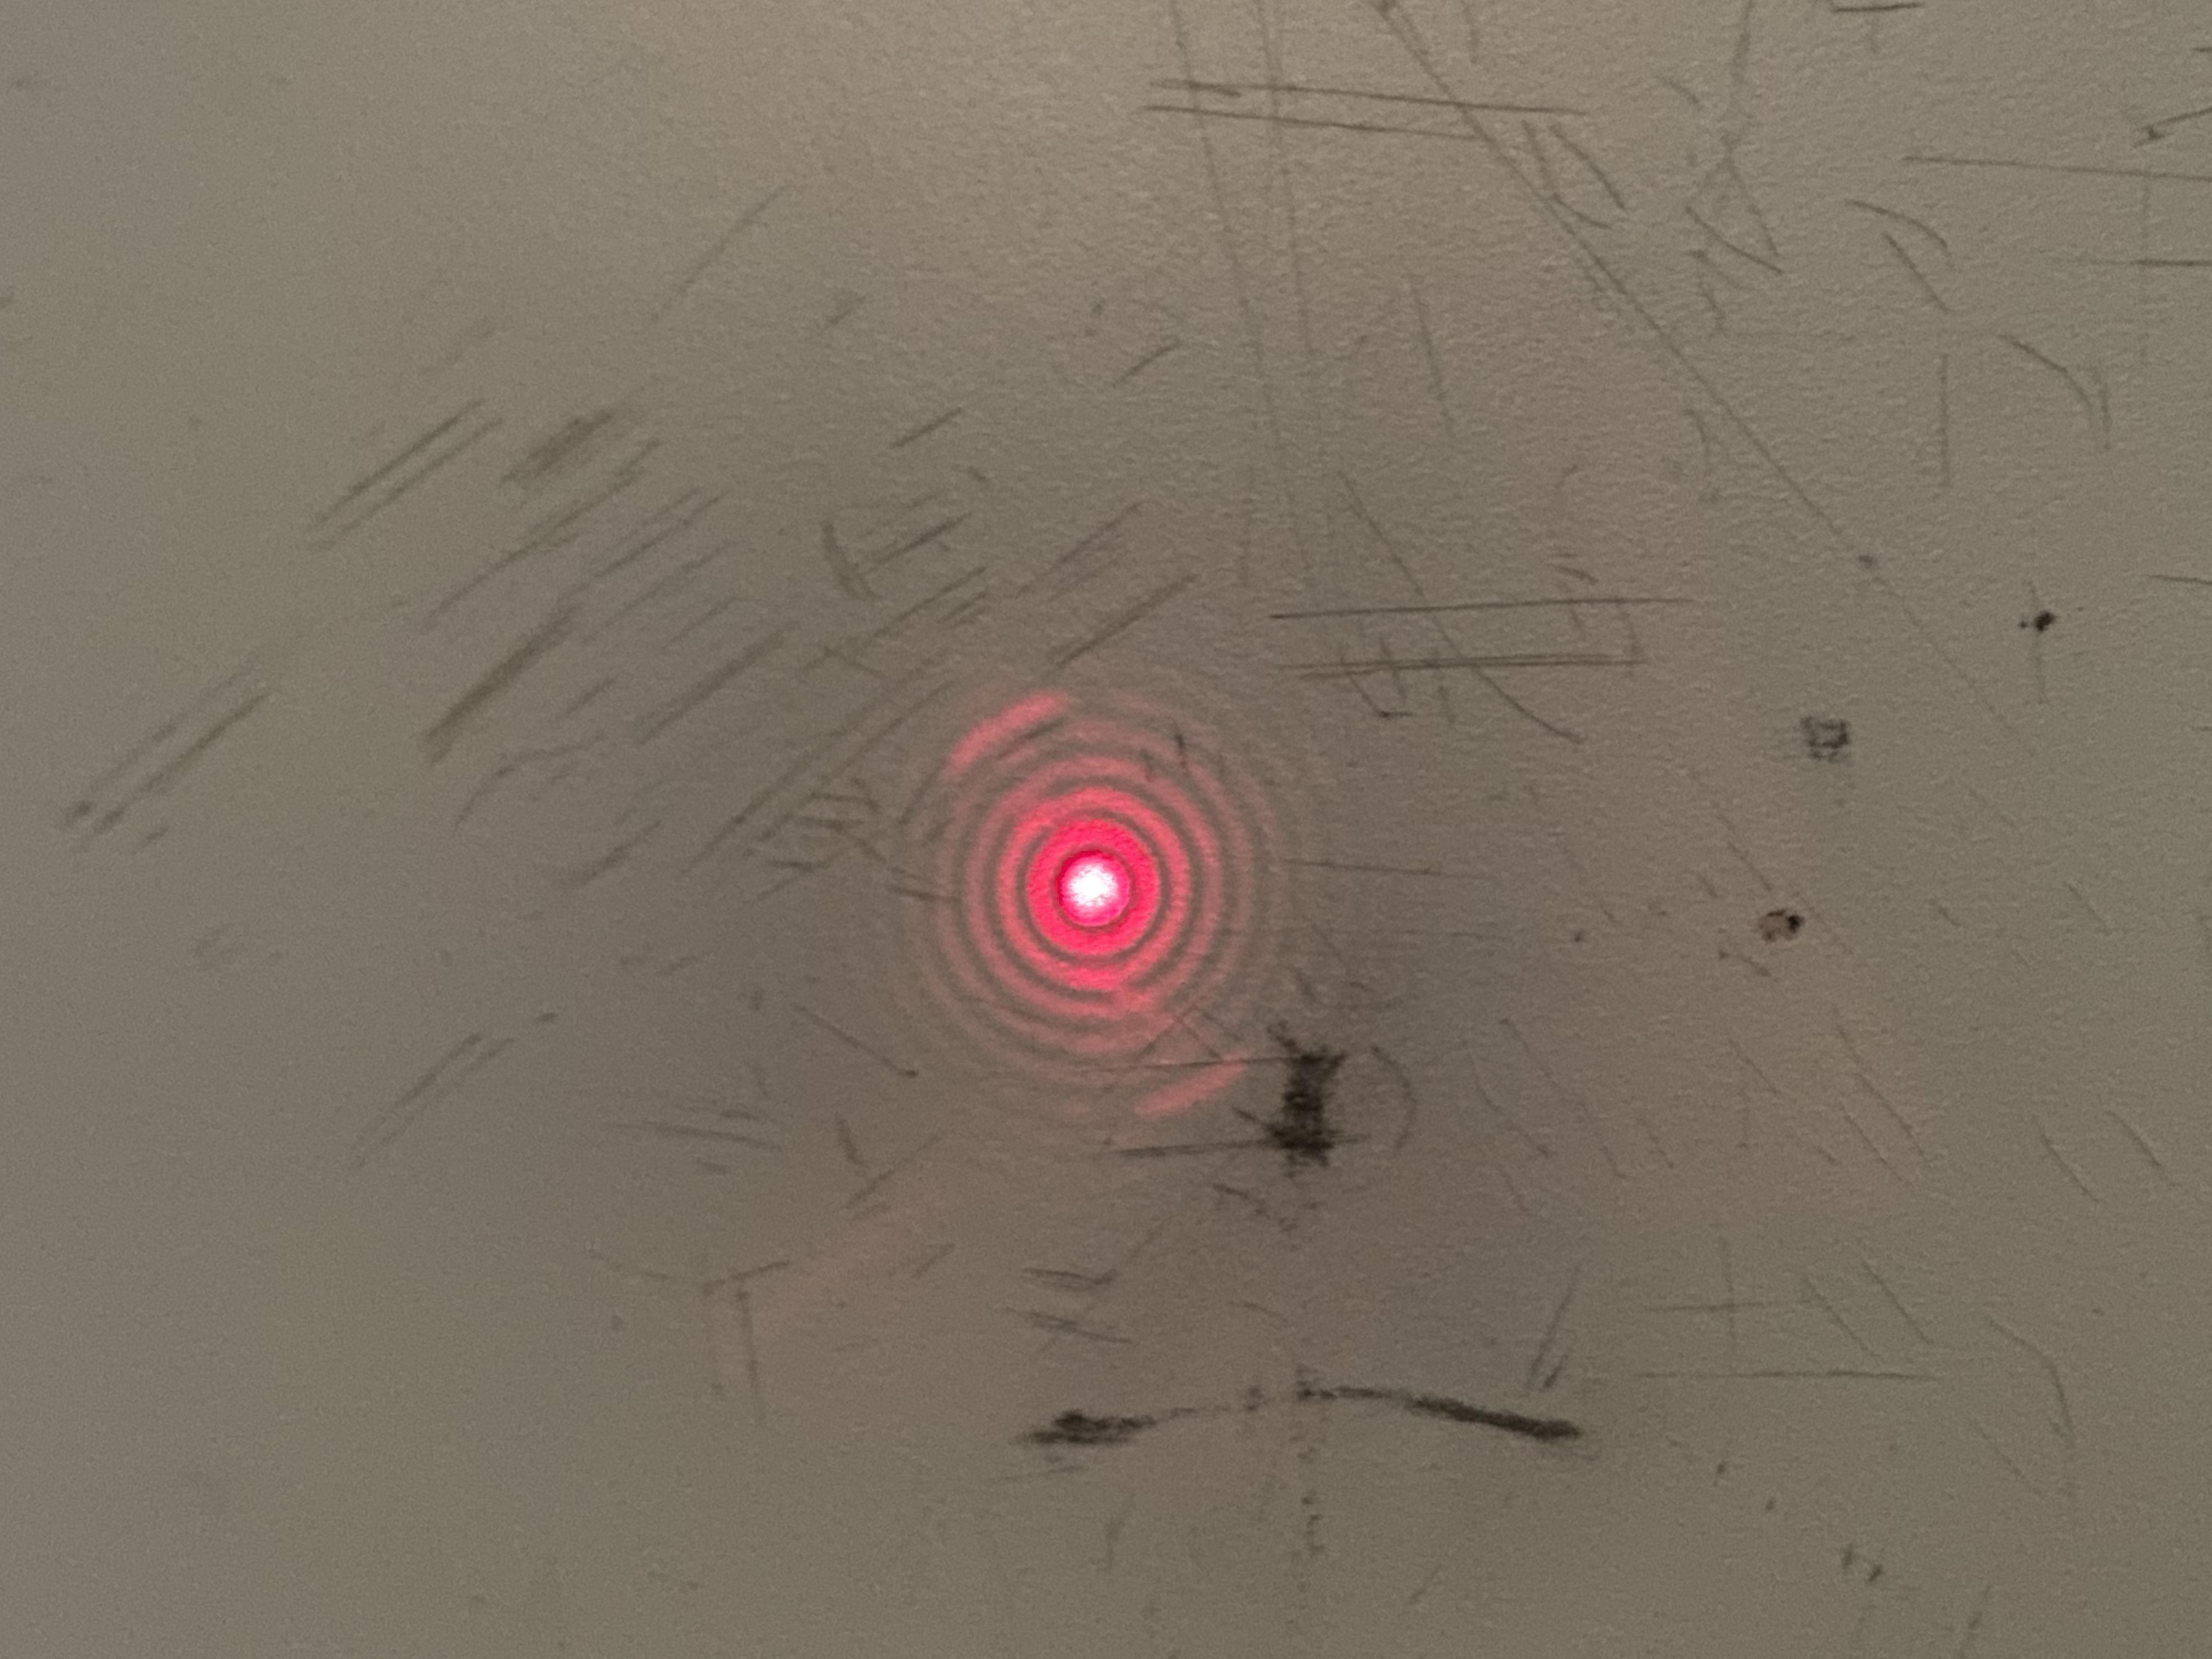
\includegraphics[height=5cm]{./pictures/photos/分划板1_小孔2.jpg}
    \caption{分划板1 小孔2}
    \label{fig:分划板1_小孔2}
  \end{subfigure}
  \label{fig:combined}
\end{figure}

\begin{figure}[H]
  \centering
  \begin{subfigure}[b]{0.45\textwidth}
    \centering
    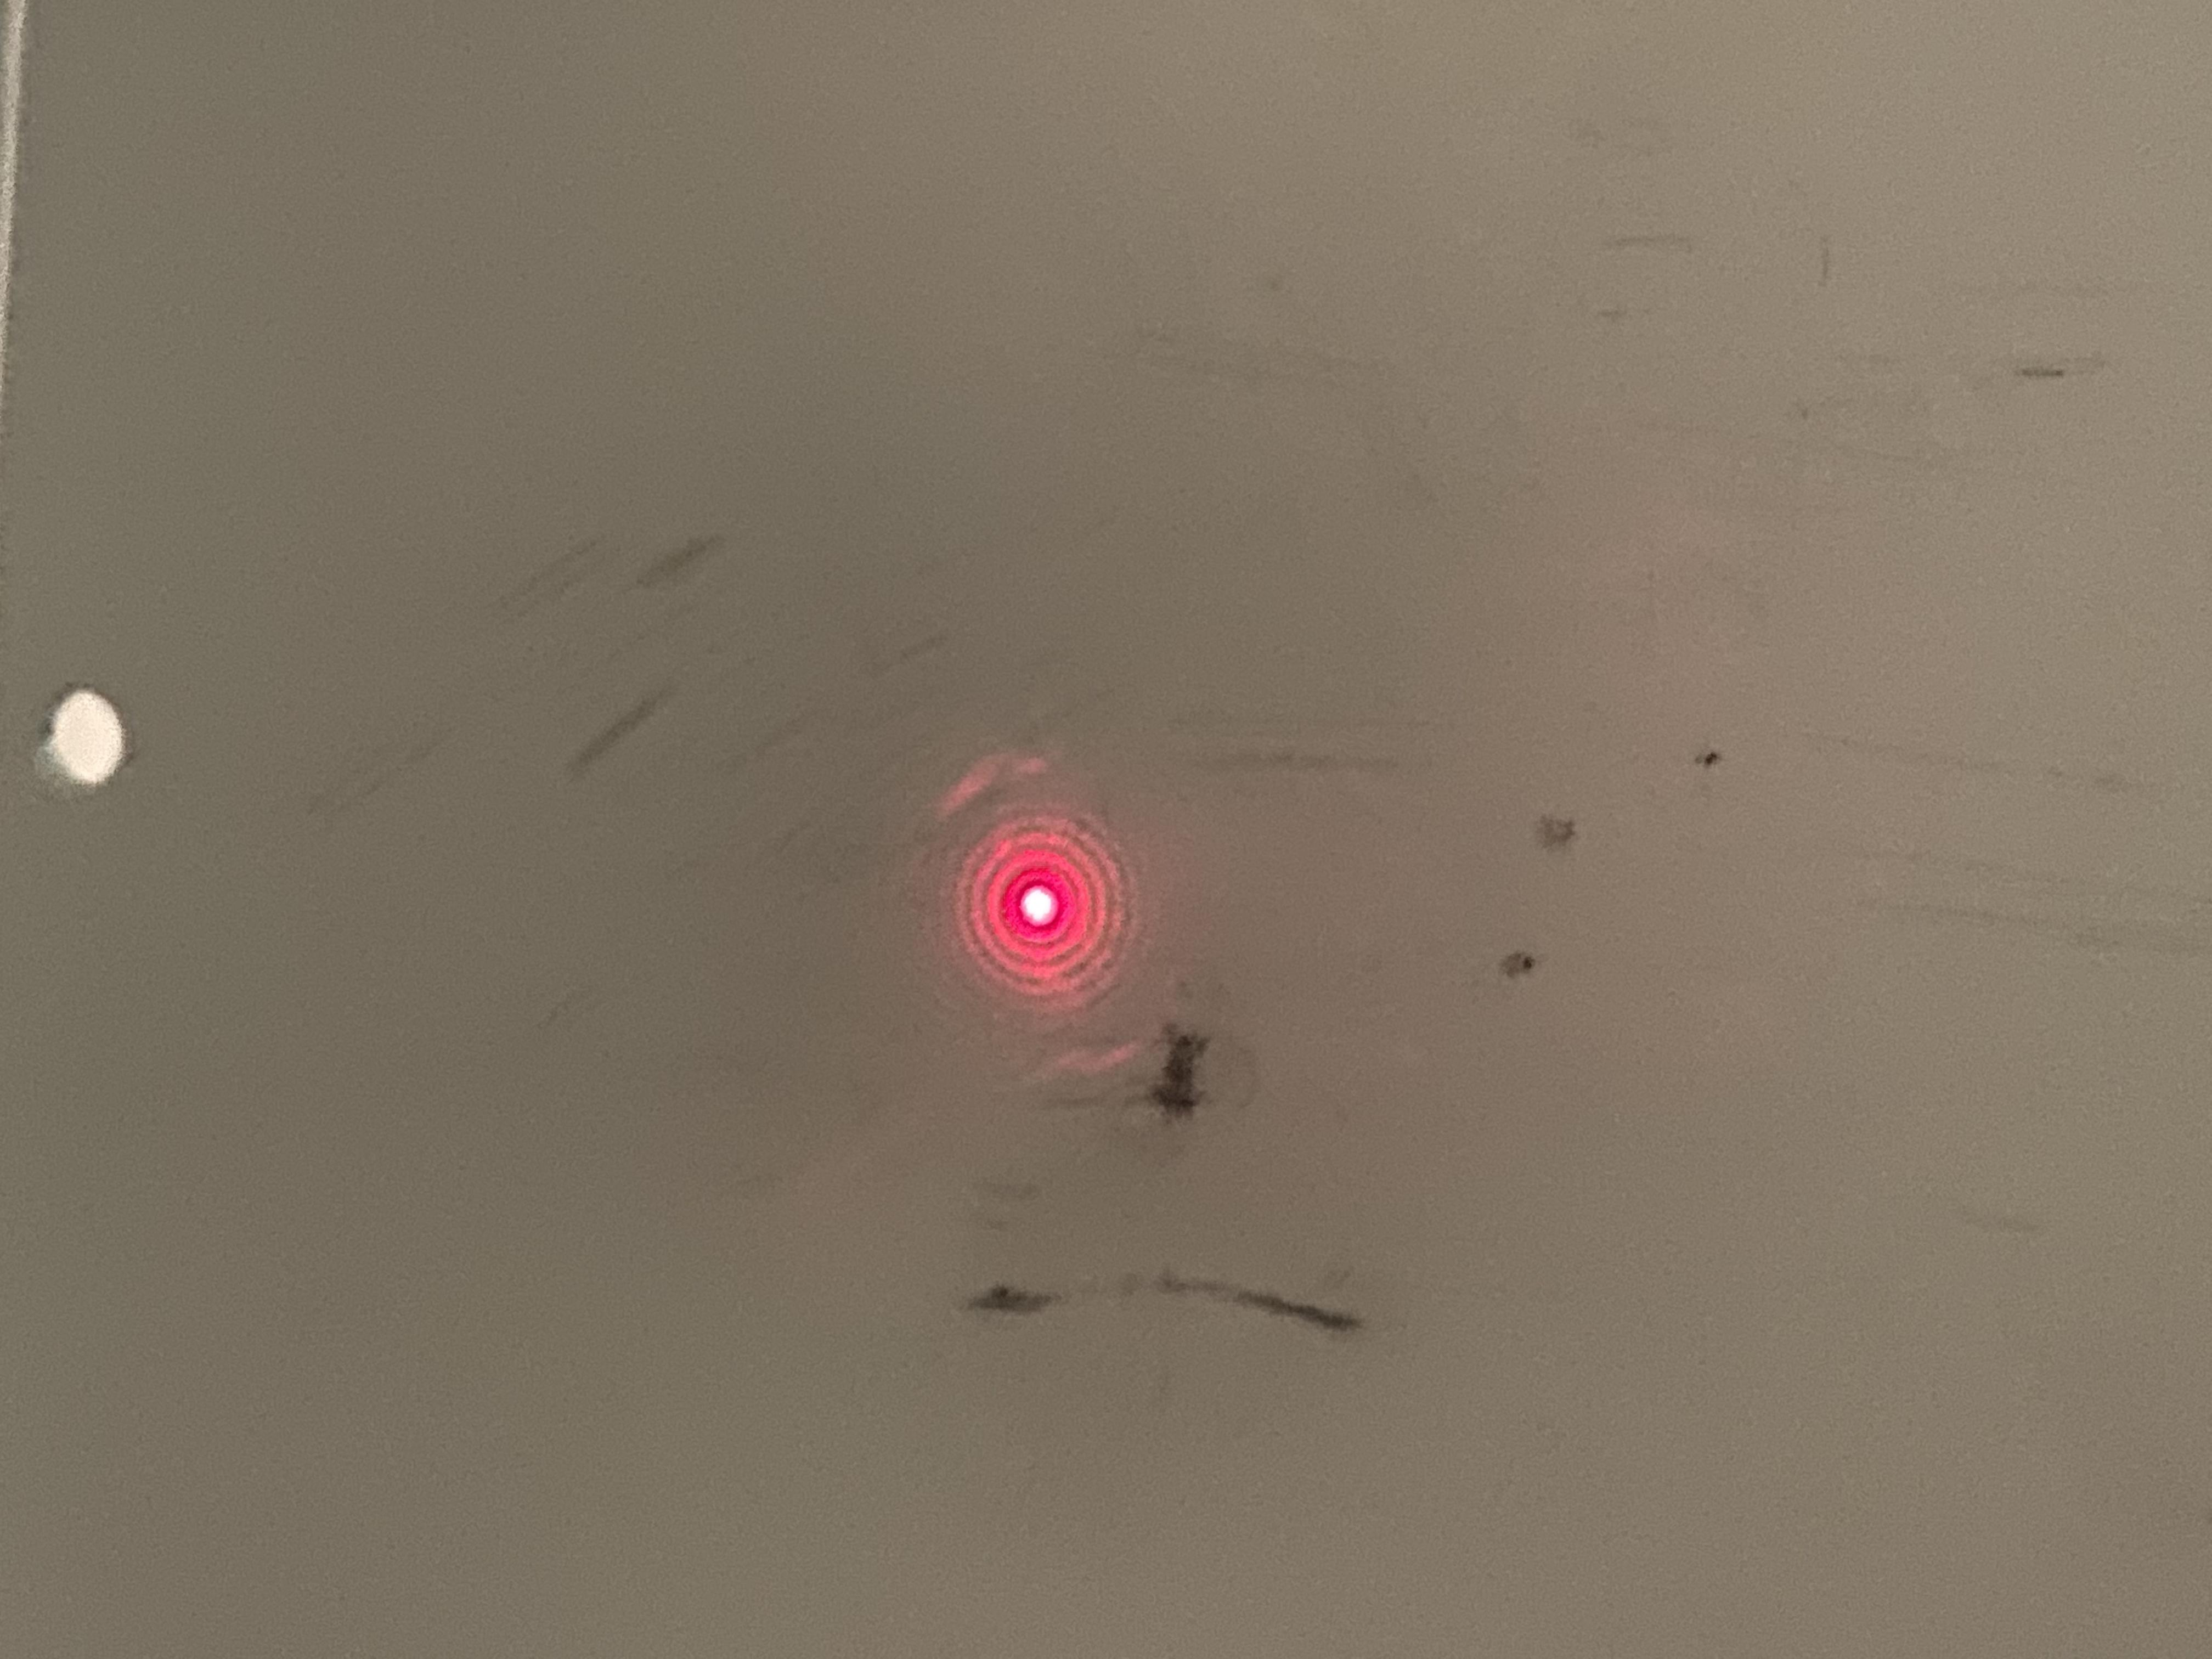
\includegraphics[height=5cm]{./pictures/photos/分划板1_小孔3.jpg}
    \caption{分划板1 小孔3}
    \label{fig:分划板1_小孔3}
  \end{subfigure}
  \hfill
  \begin{subfigure}[b]{0.45\textwidth}
    \centering
    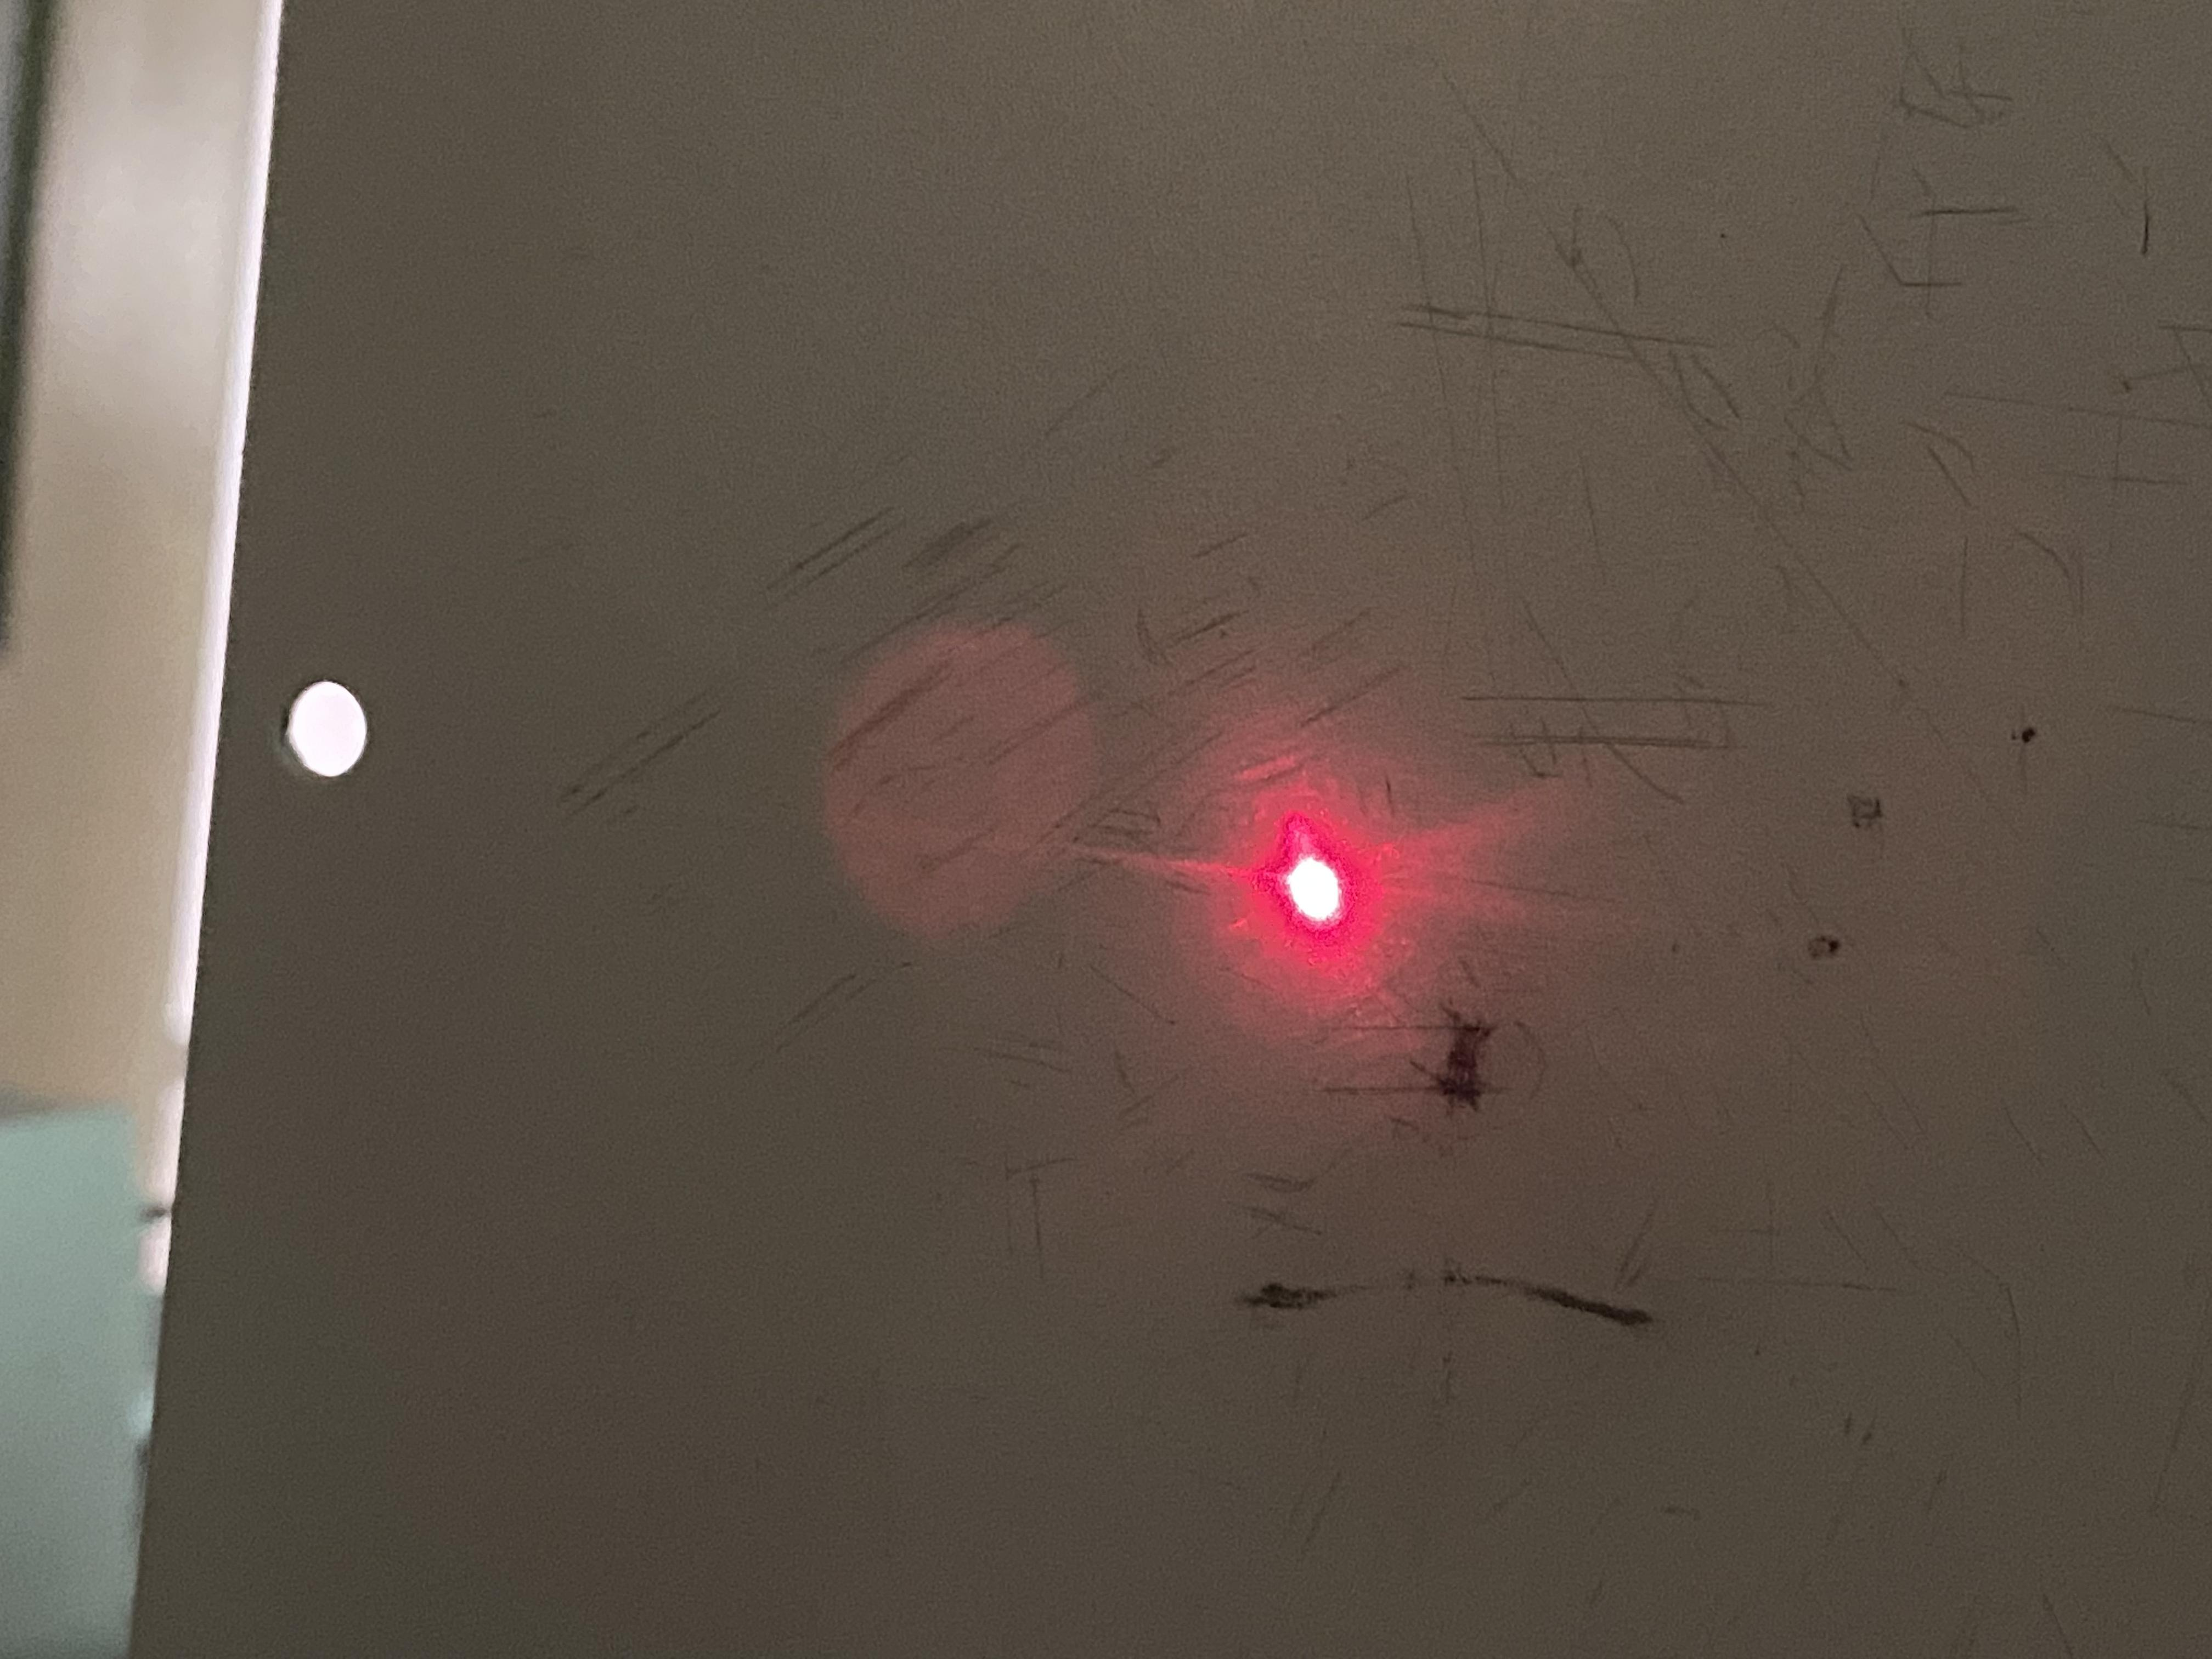
\includegraphics[height=5cm]{./pictures/photos/分划板1_小屏1.jpg}
    \caption{分划板1 小屏1}
    \label{fig:分划板1_小屏1}
  \end{subfigure}
  \label{fig:combined}
\end{figure}

\begin{figure}[H]
  \centering
  \begin{subfigure}[b]{0.45\textwidth}
    \centering
    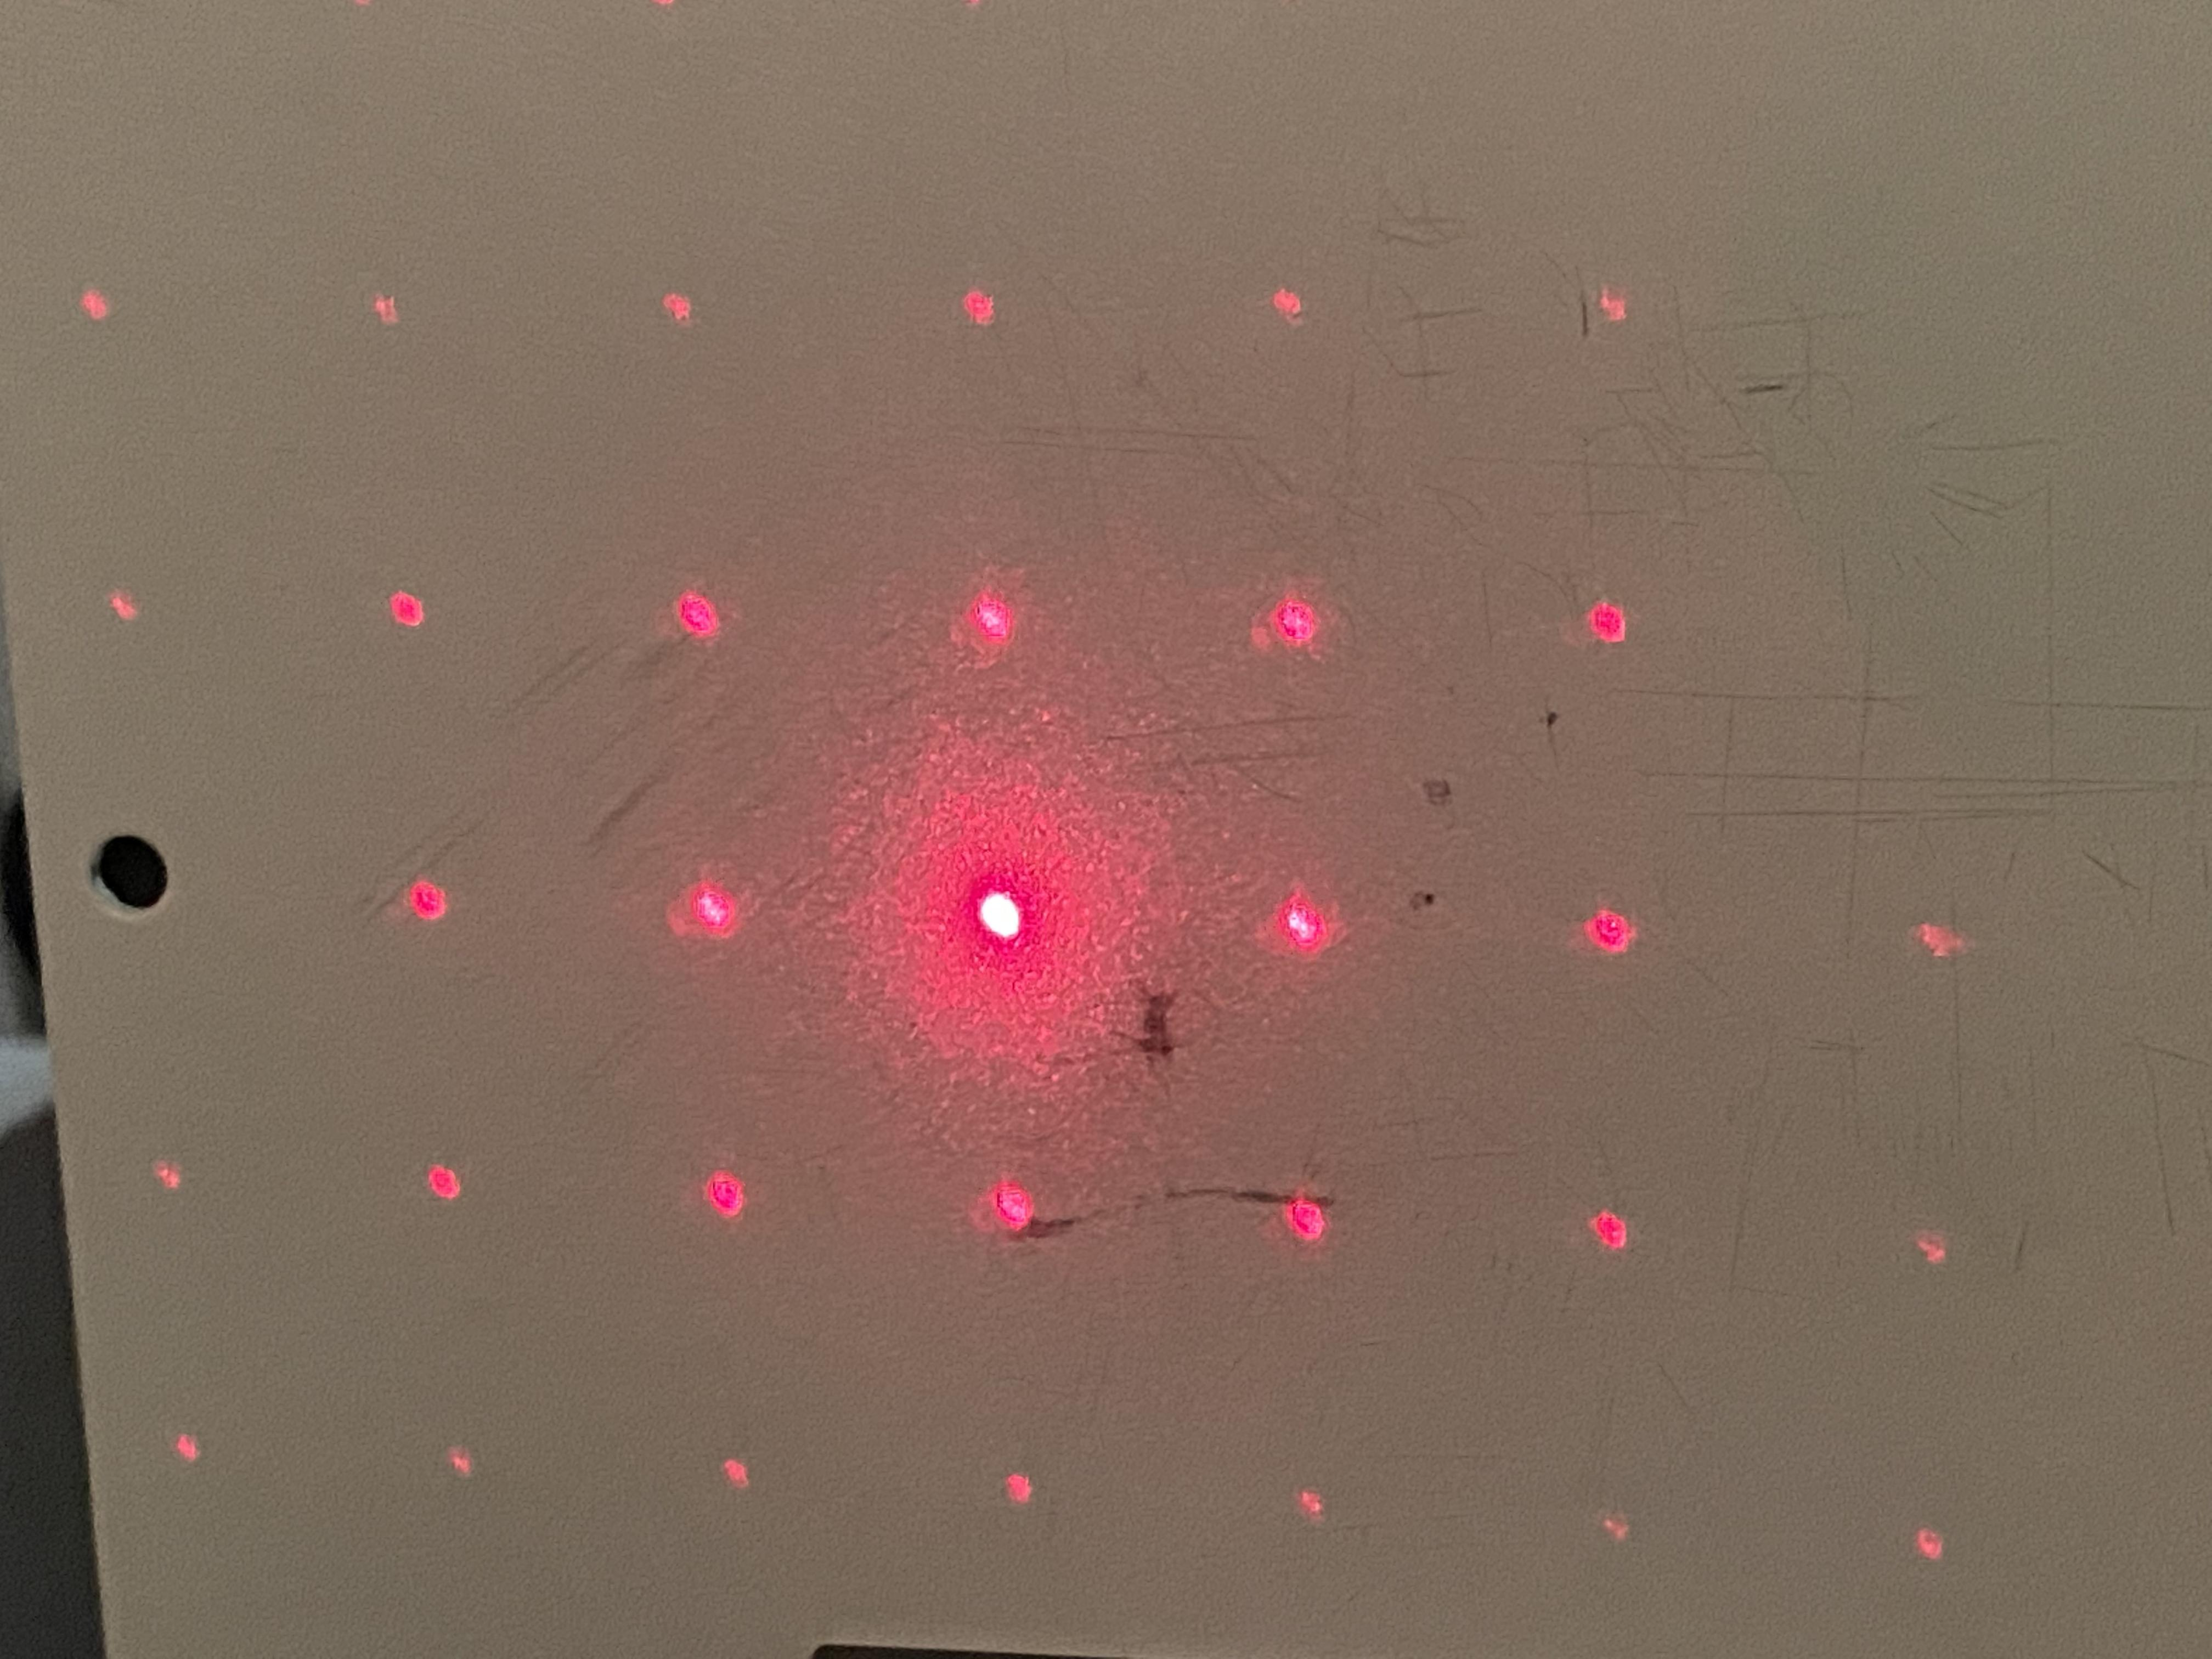
\includegraphics[height=5cm]{./pictures/photos/分划板2_光栅1.jpg}
    \caption{分划板2 光栅1}
    \label{fig:分划板2_光栅1}
  \end{subfigure}
  \hfill
  \begin{subfigure}[b]{0.45\textwidth}
    \centering
    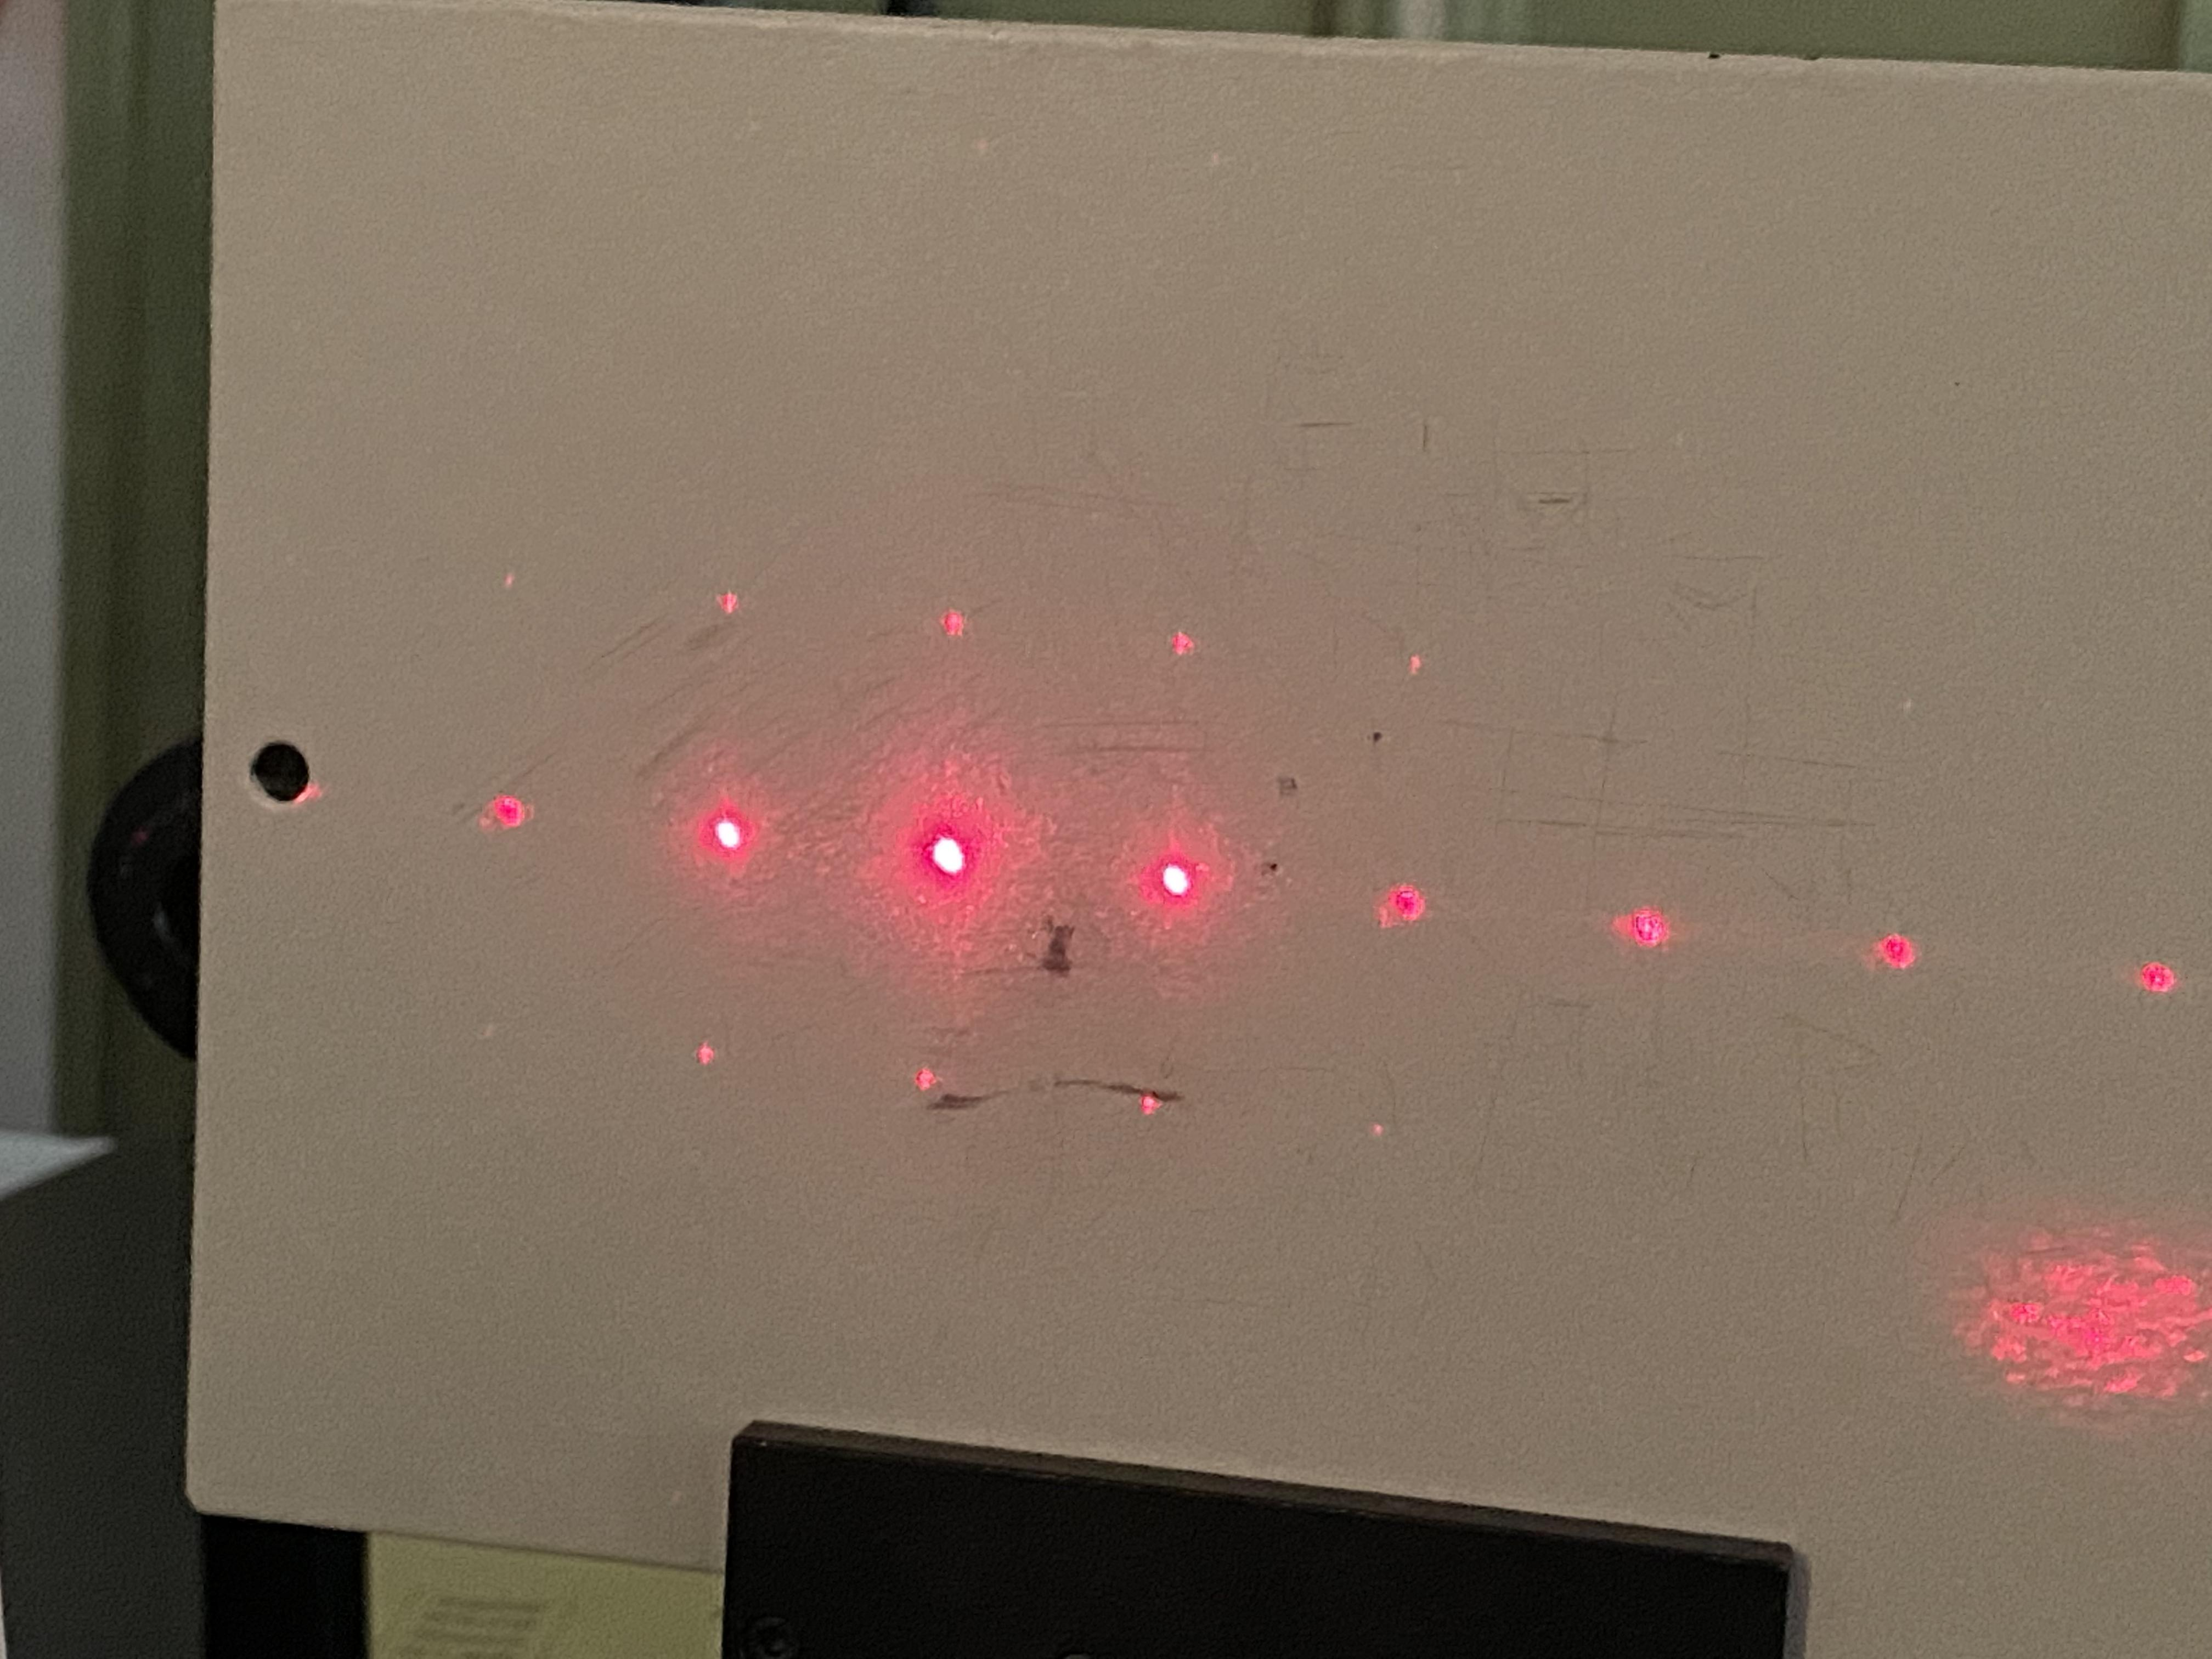
\includegraphics[height=5cm]{./pictures/photos/分划板2_光栅2.jpg}
    \caption{分划板2 光栅2}
    \label{fig:分划板2_光栅2}
  \end{subfigure}
  \label{fig:combined}
\end{figure}

\begin{figure}[H]
  \centering
  \begin{subfigure}[b]{0.45\textwidth}
    \centering
    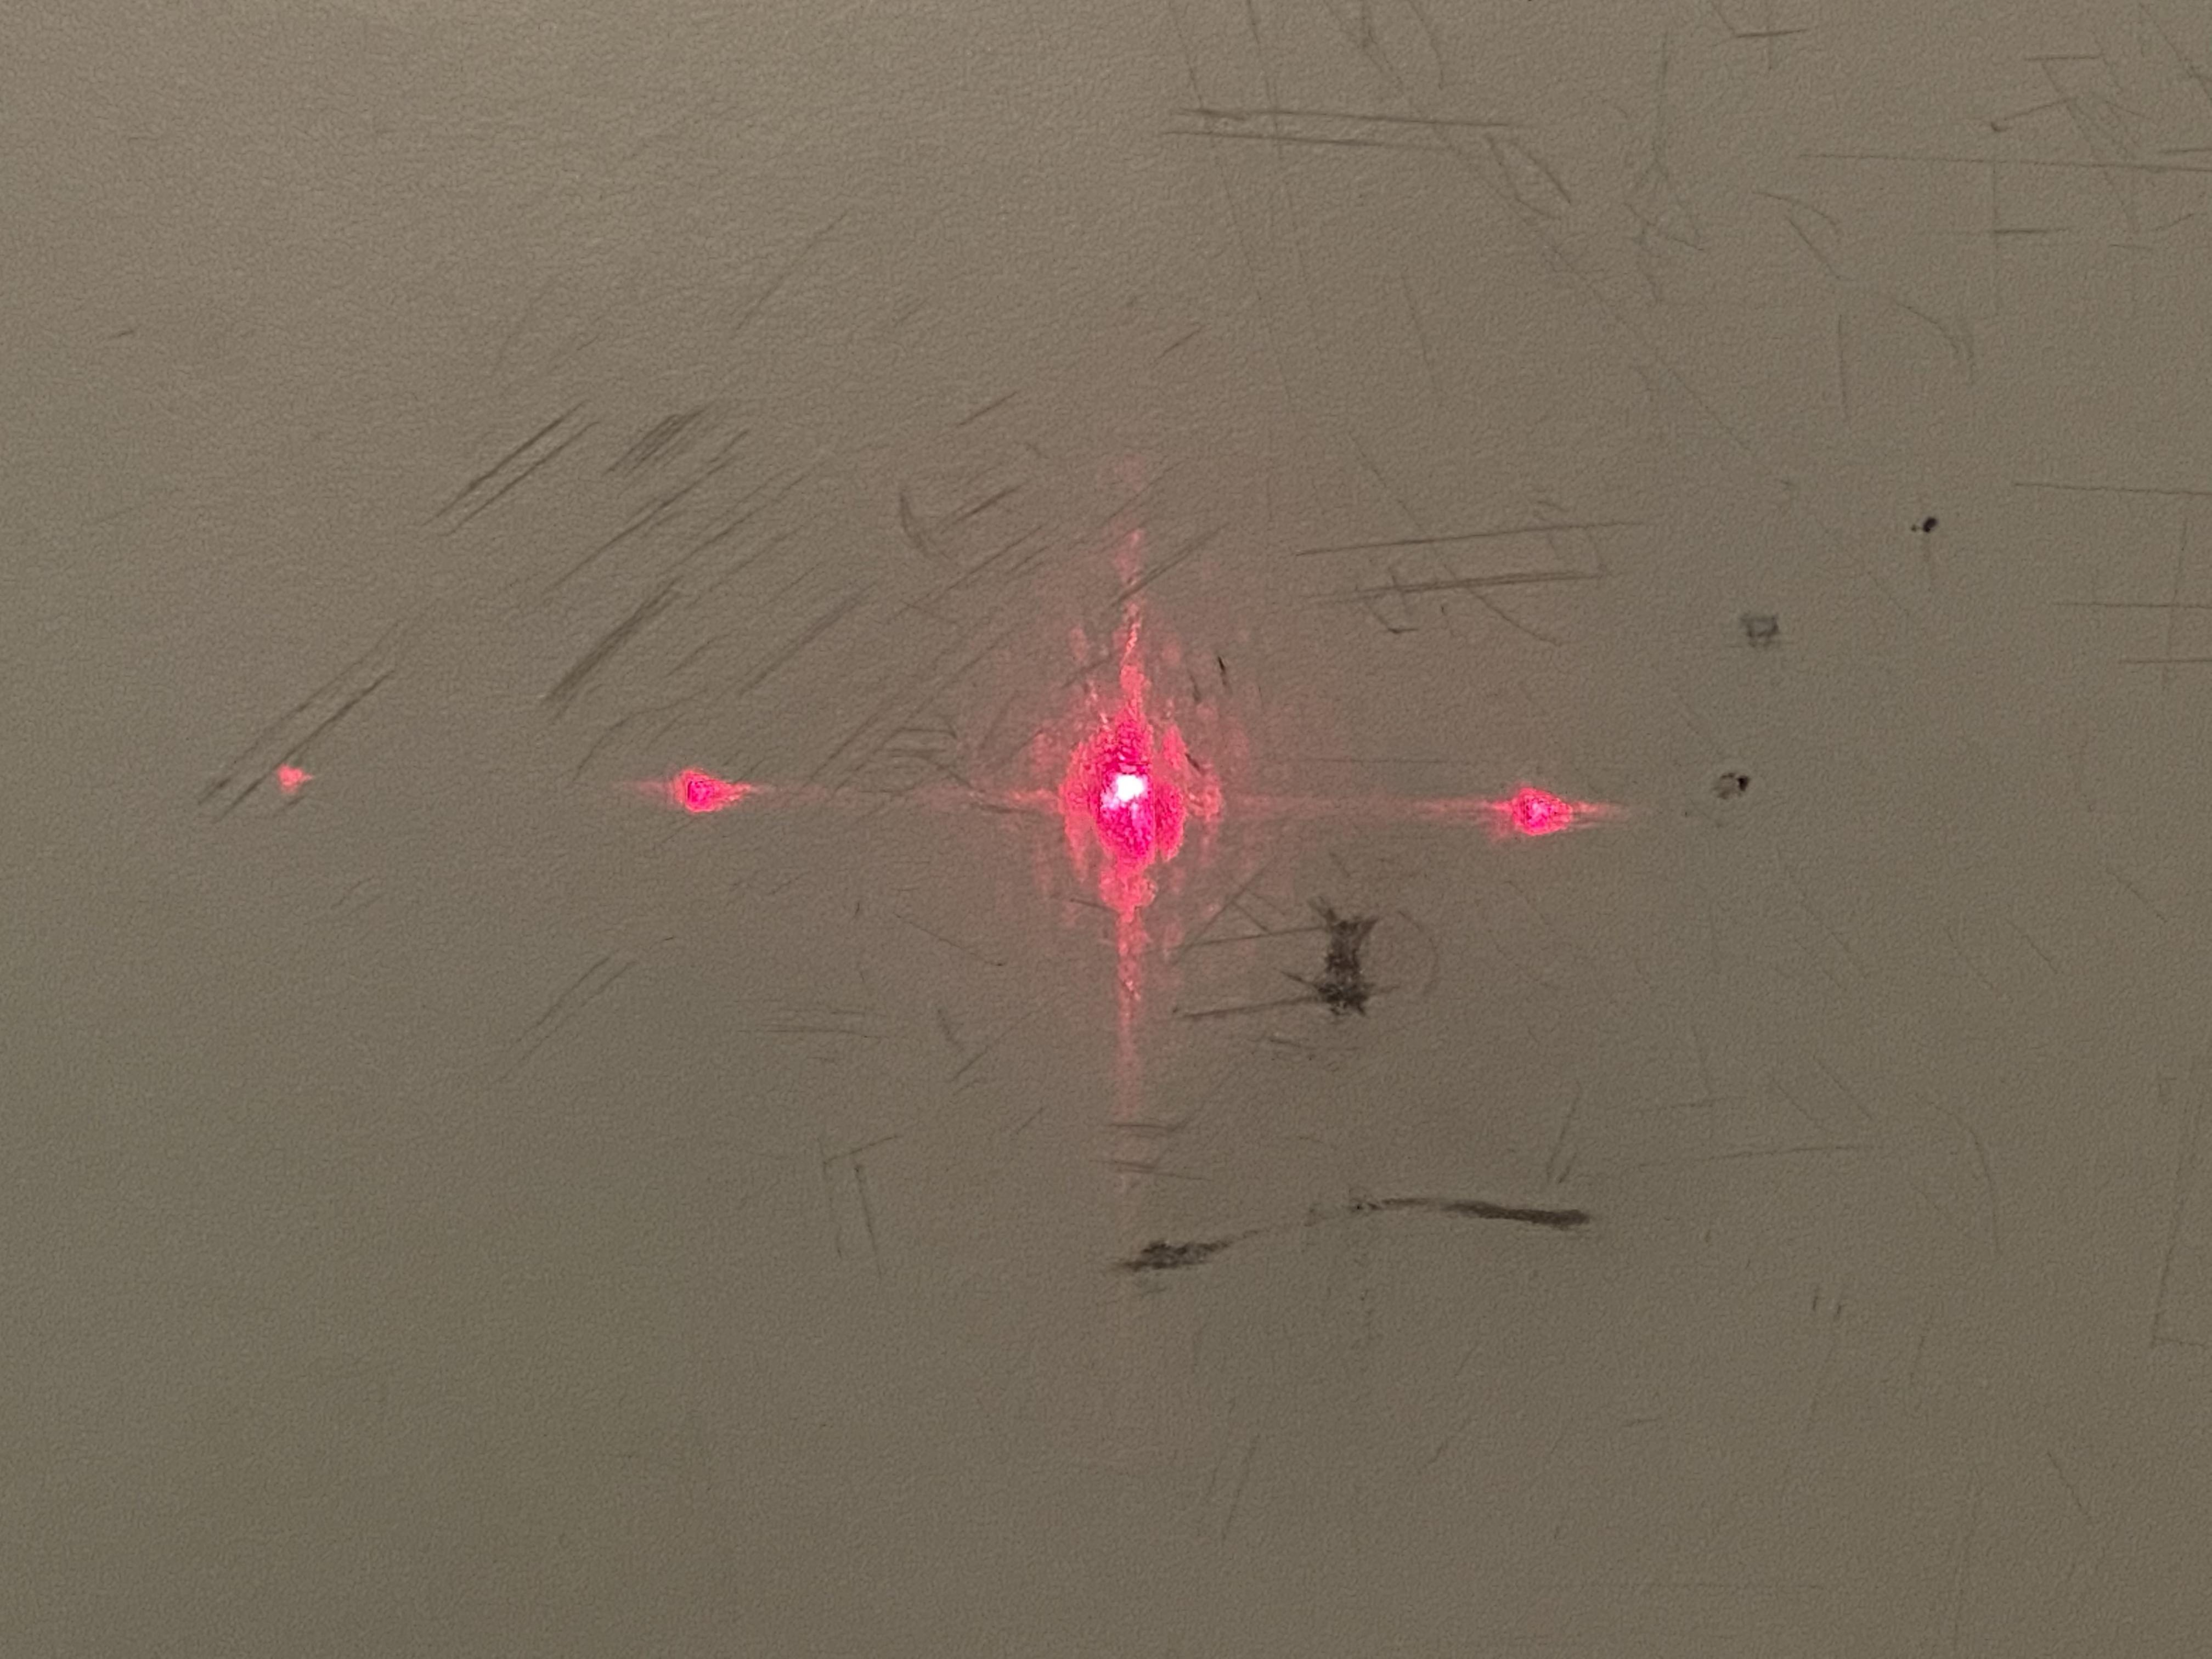
\includegraphics[height=5cm]{./pictures/photos/分划板2_双孔1.jpg}
    \caption{分划板2 双孔1}
    \label{fig:分划板2_双孔1}
  \end{subfigure}
  \hfill
  \begin{subfigure}[b]{0.45\textwidth}
    \centering
    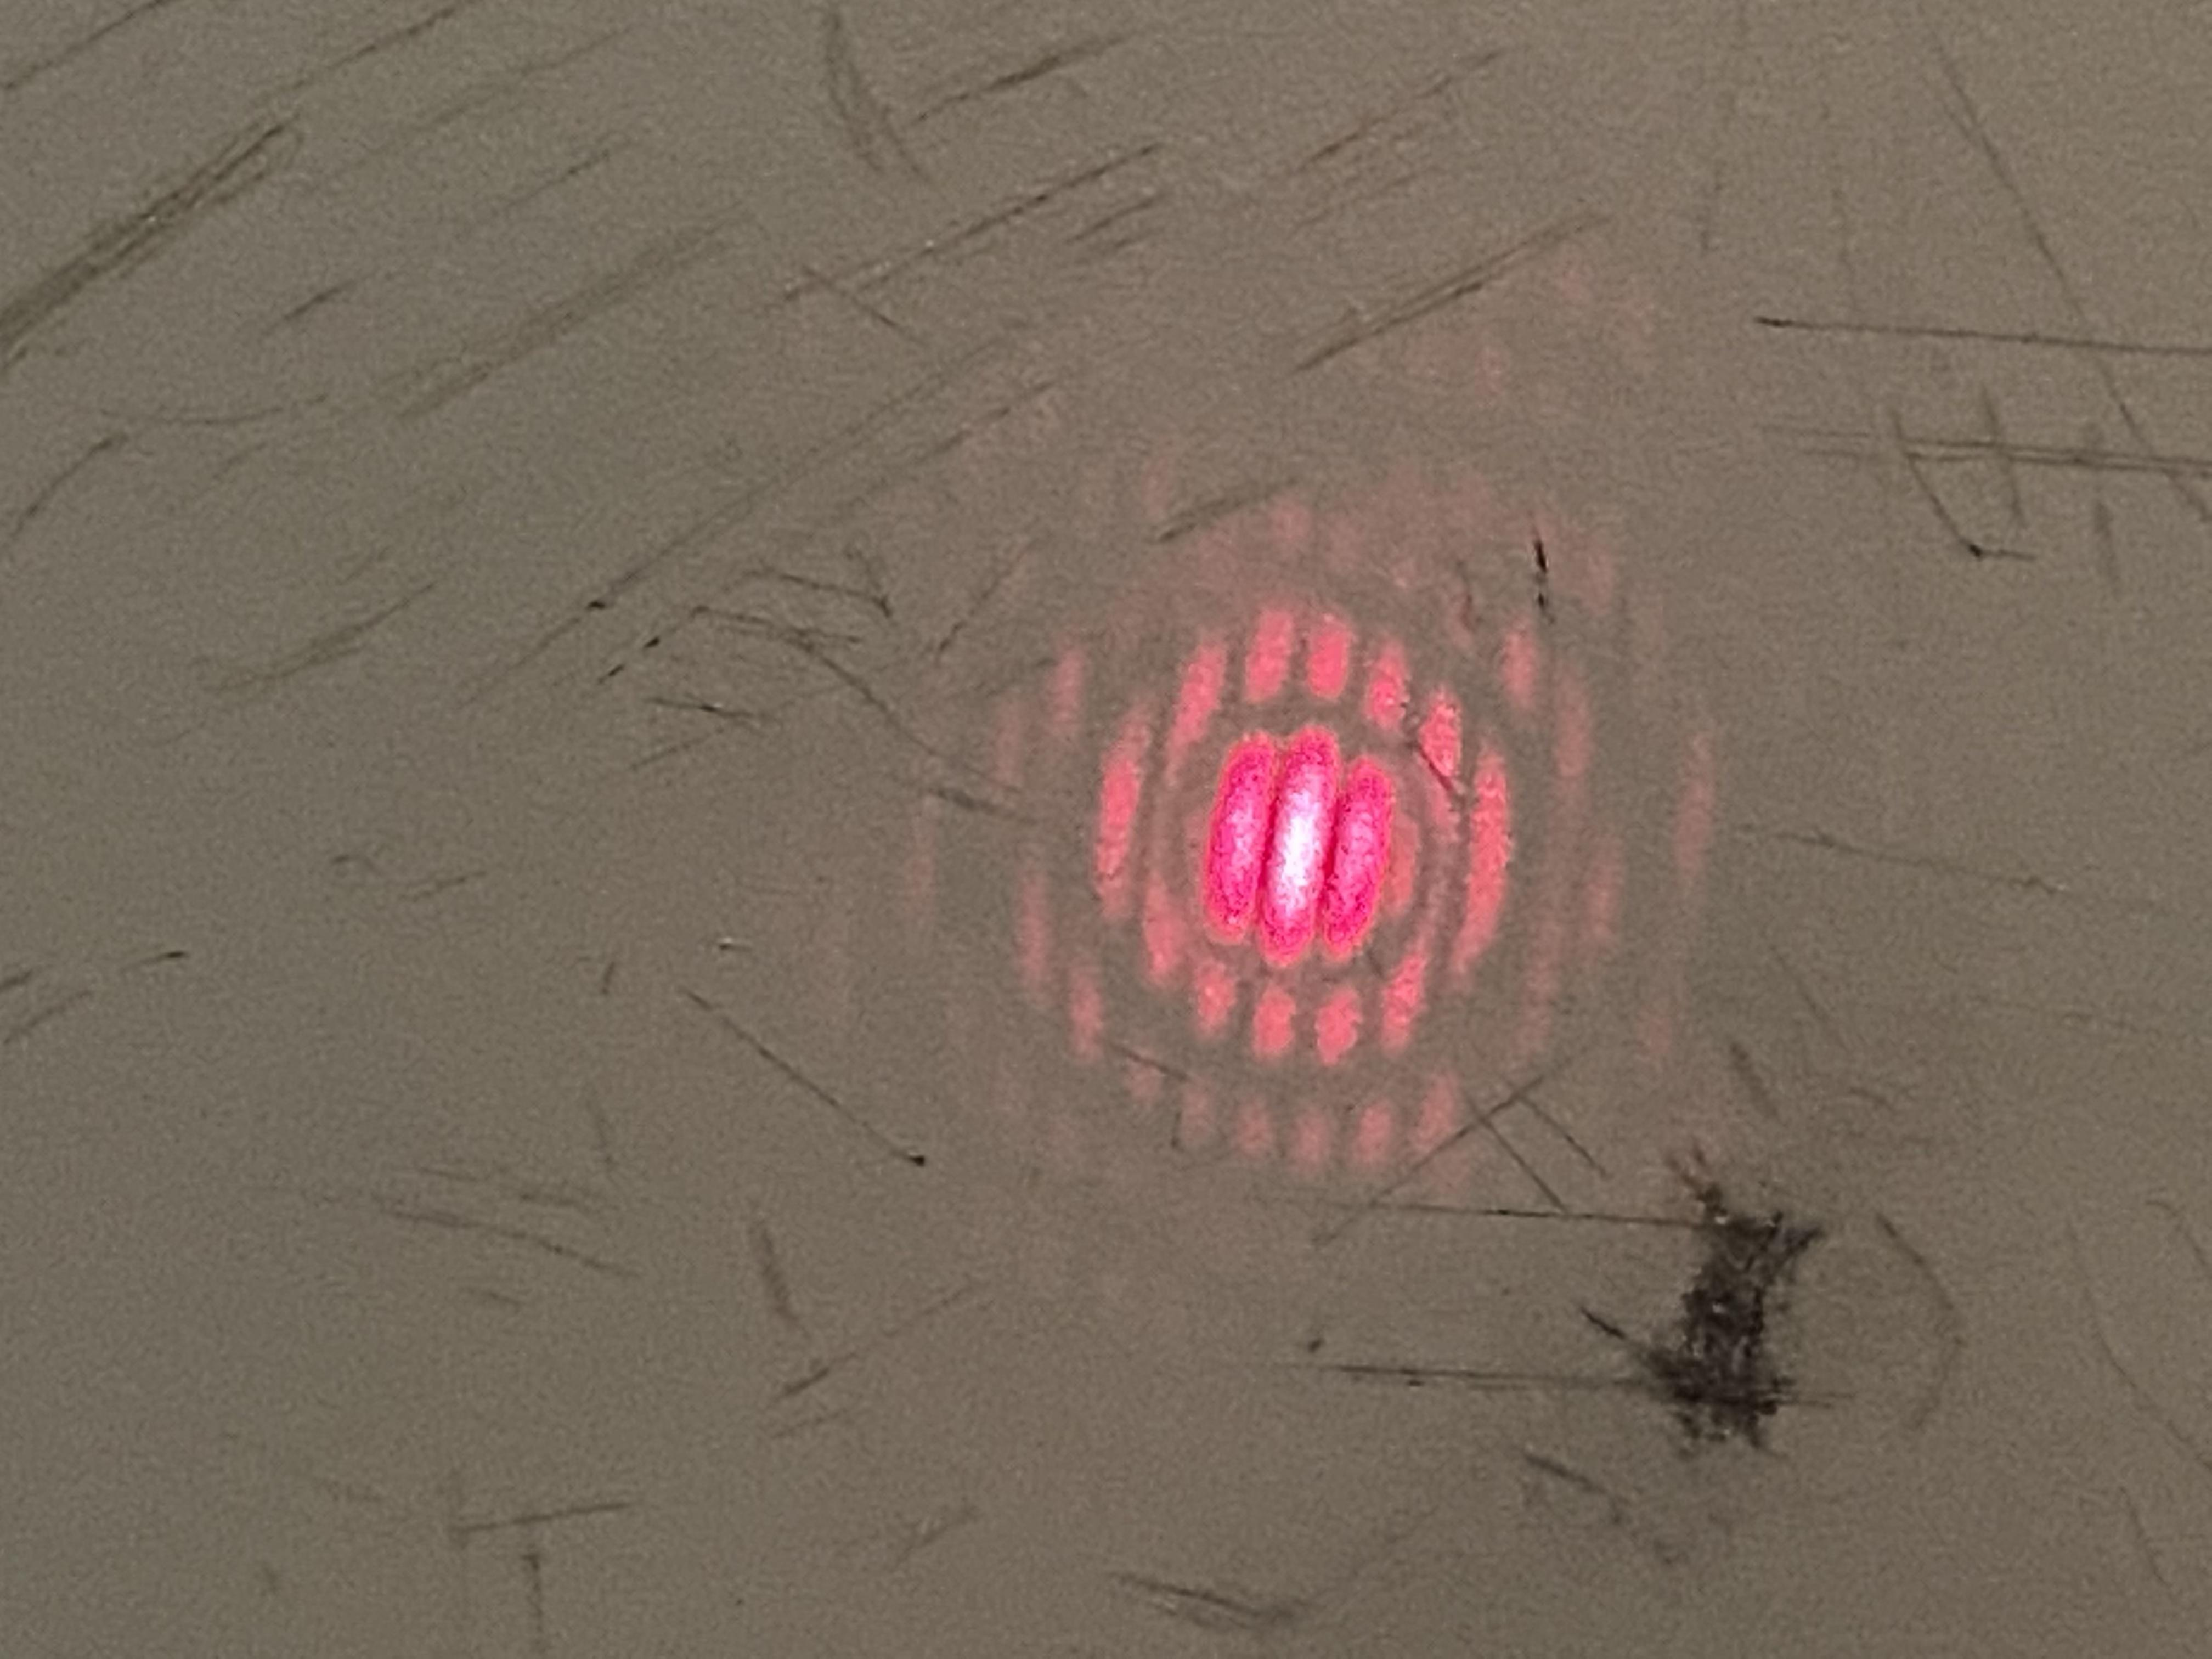
\includegraphics[height=5cm]{./pictures/photos/分划板2_双孔2.jpg}
    \caption{分划板2 双孔2}
    \label{fig:分划板2_双孔2}
  \end{subfigure}
  \label{fig:combined}
\end{figure}

\begin{figure}[H]
  \centering
  \begin{subfigure}[b]{0.45\textwidth}
    \centering
    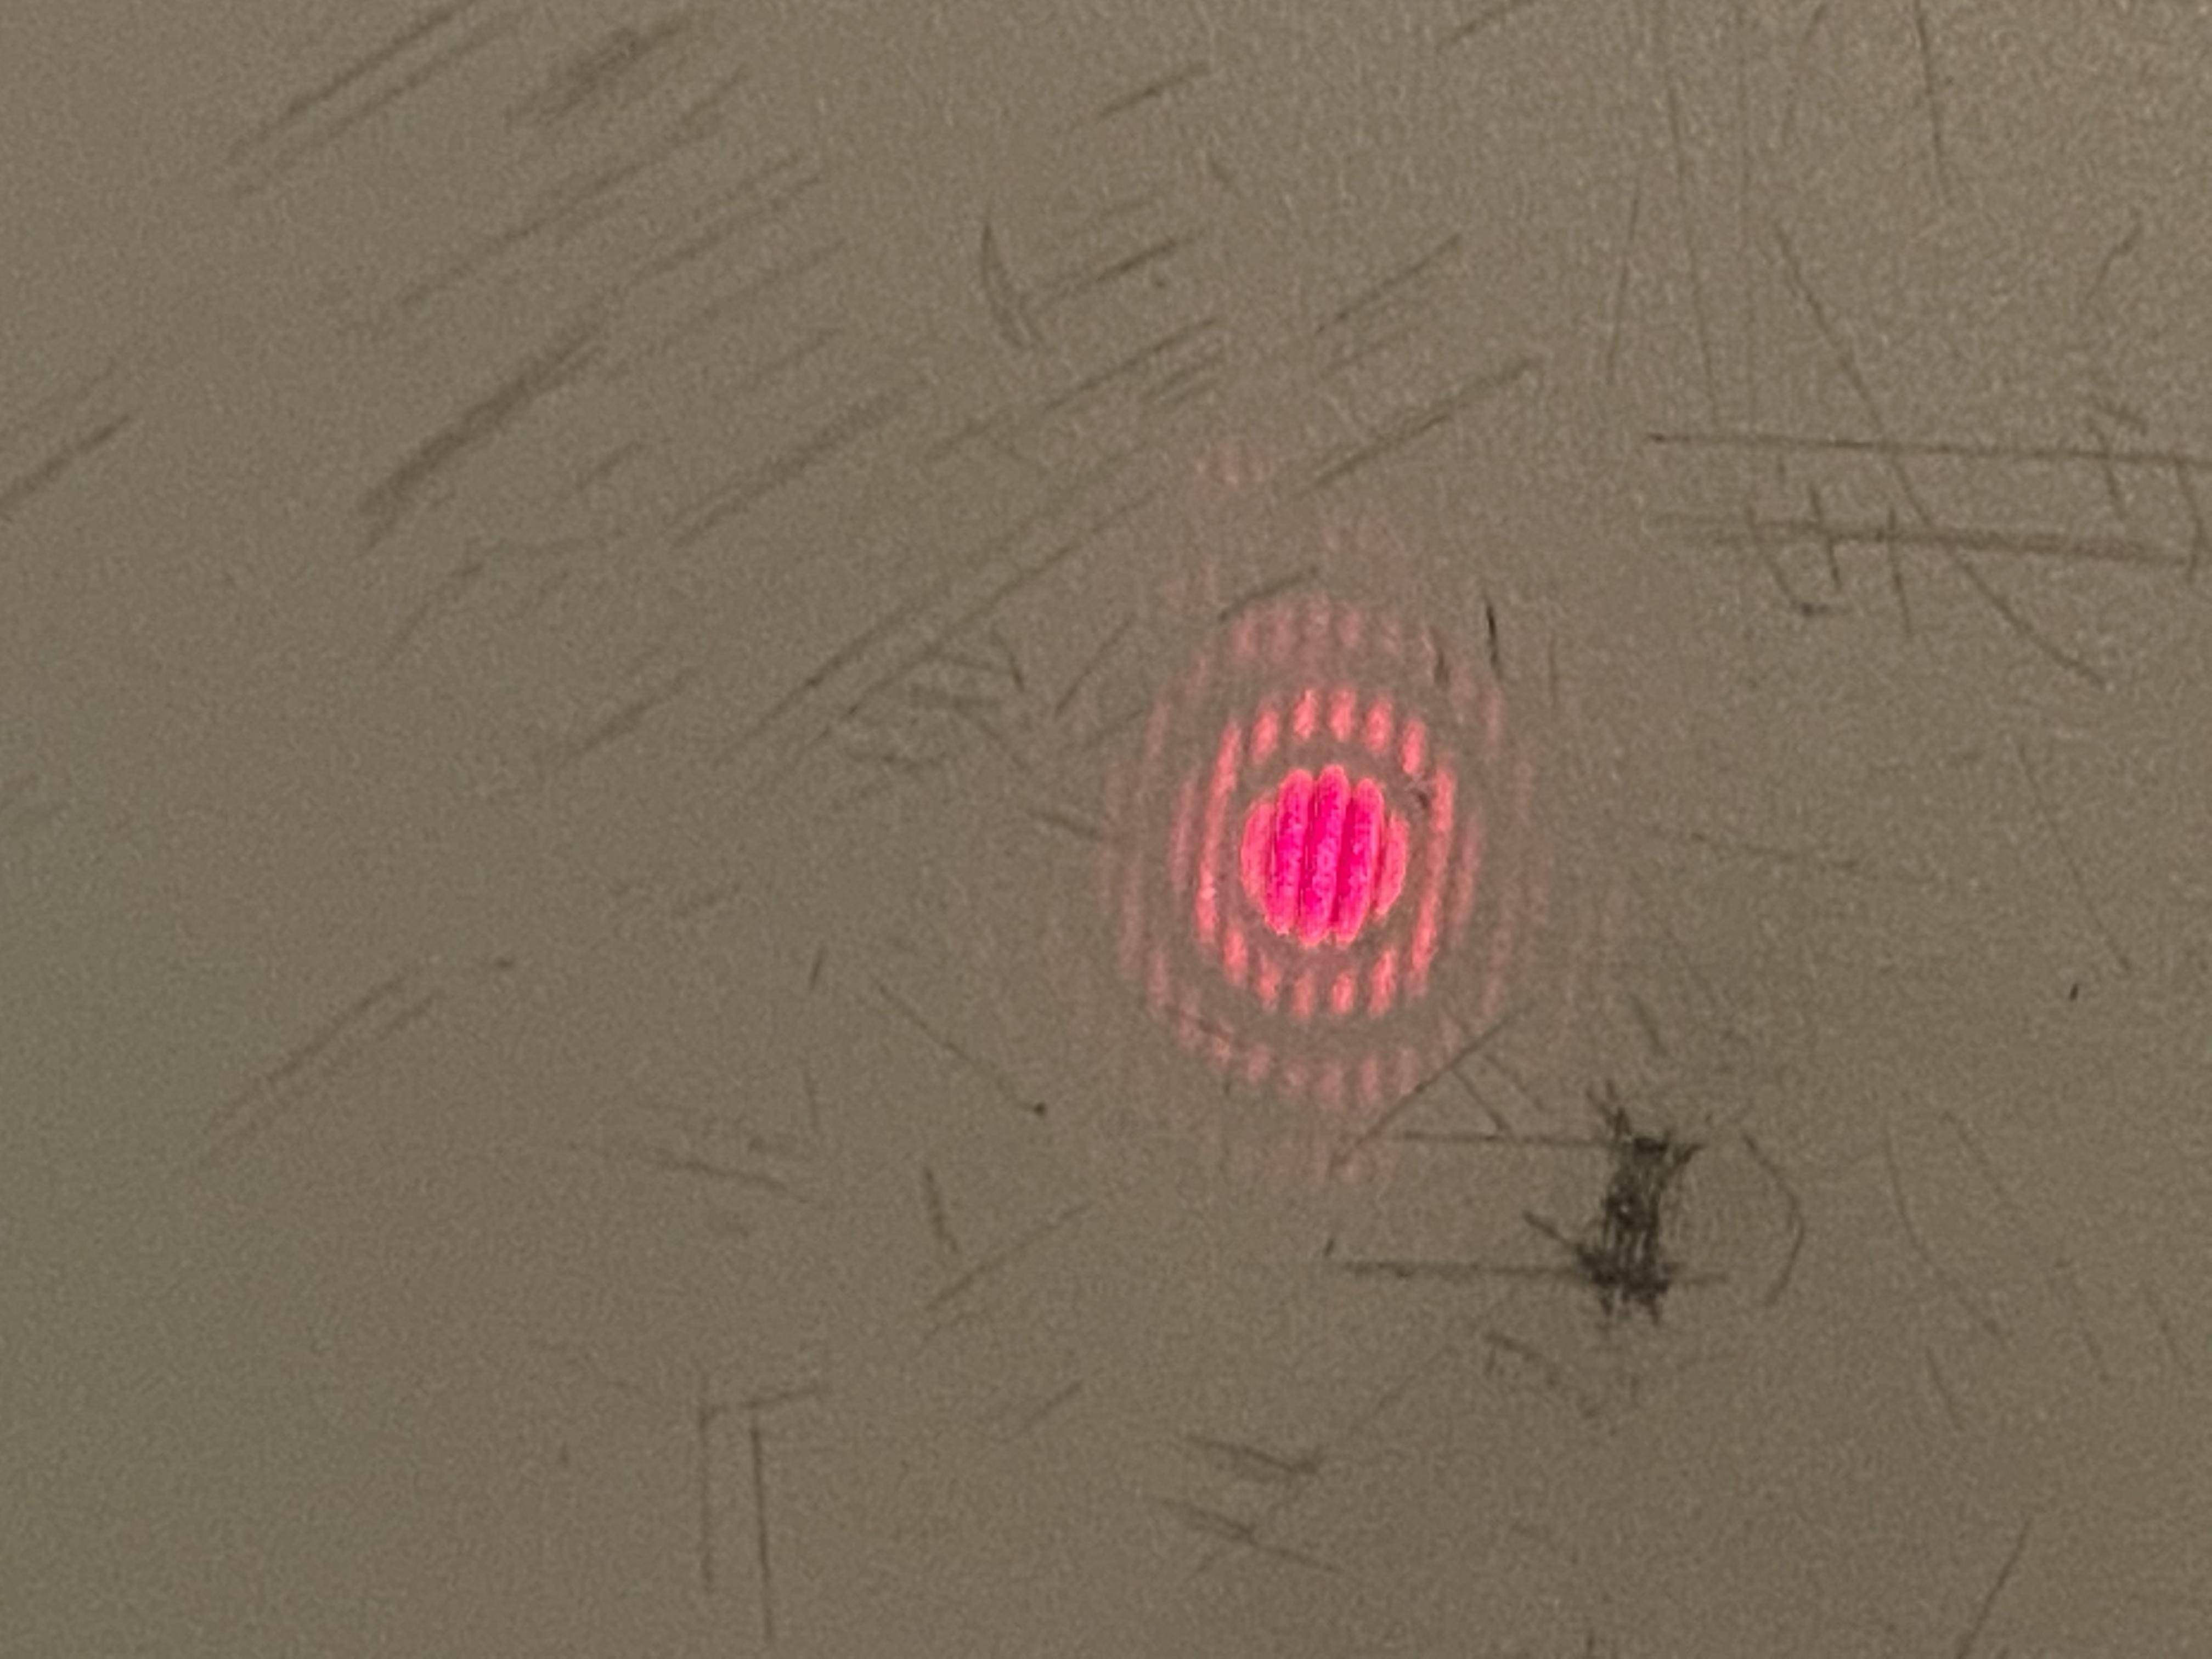
\includegraphics[height=5cm]{./pictures/photos/分划板2_双孔3.jpg}
    \caption{分划板2 双孔3}
    \label{fig:分划板2_双孔3}     
  \end{subfigure}
  \hfill
  \begin{subfigure}[b]{0.45\textwidth}
    \centering
    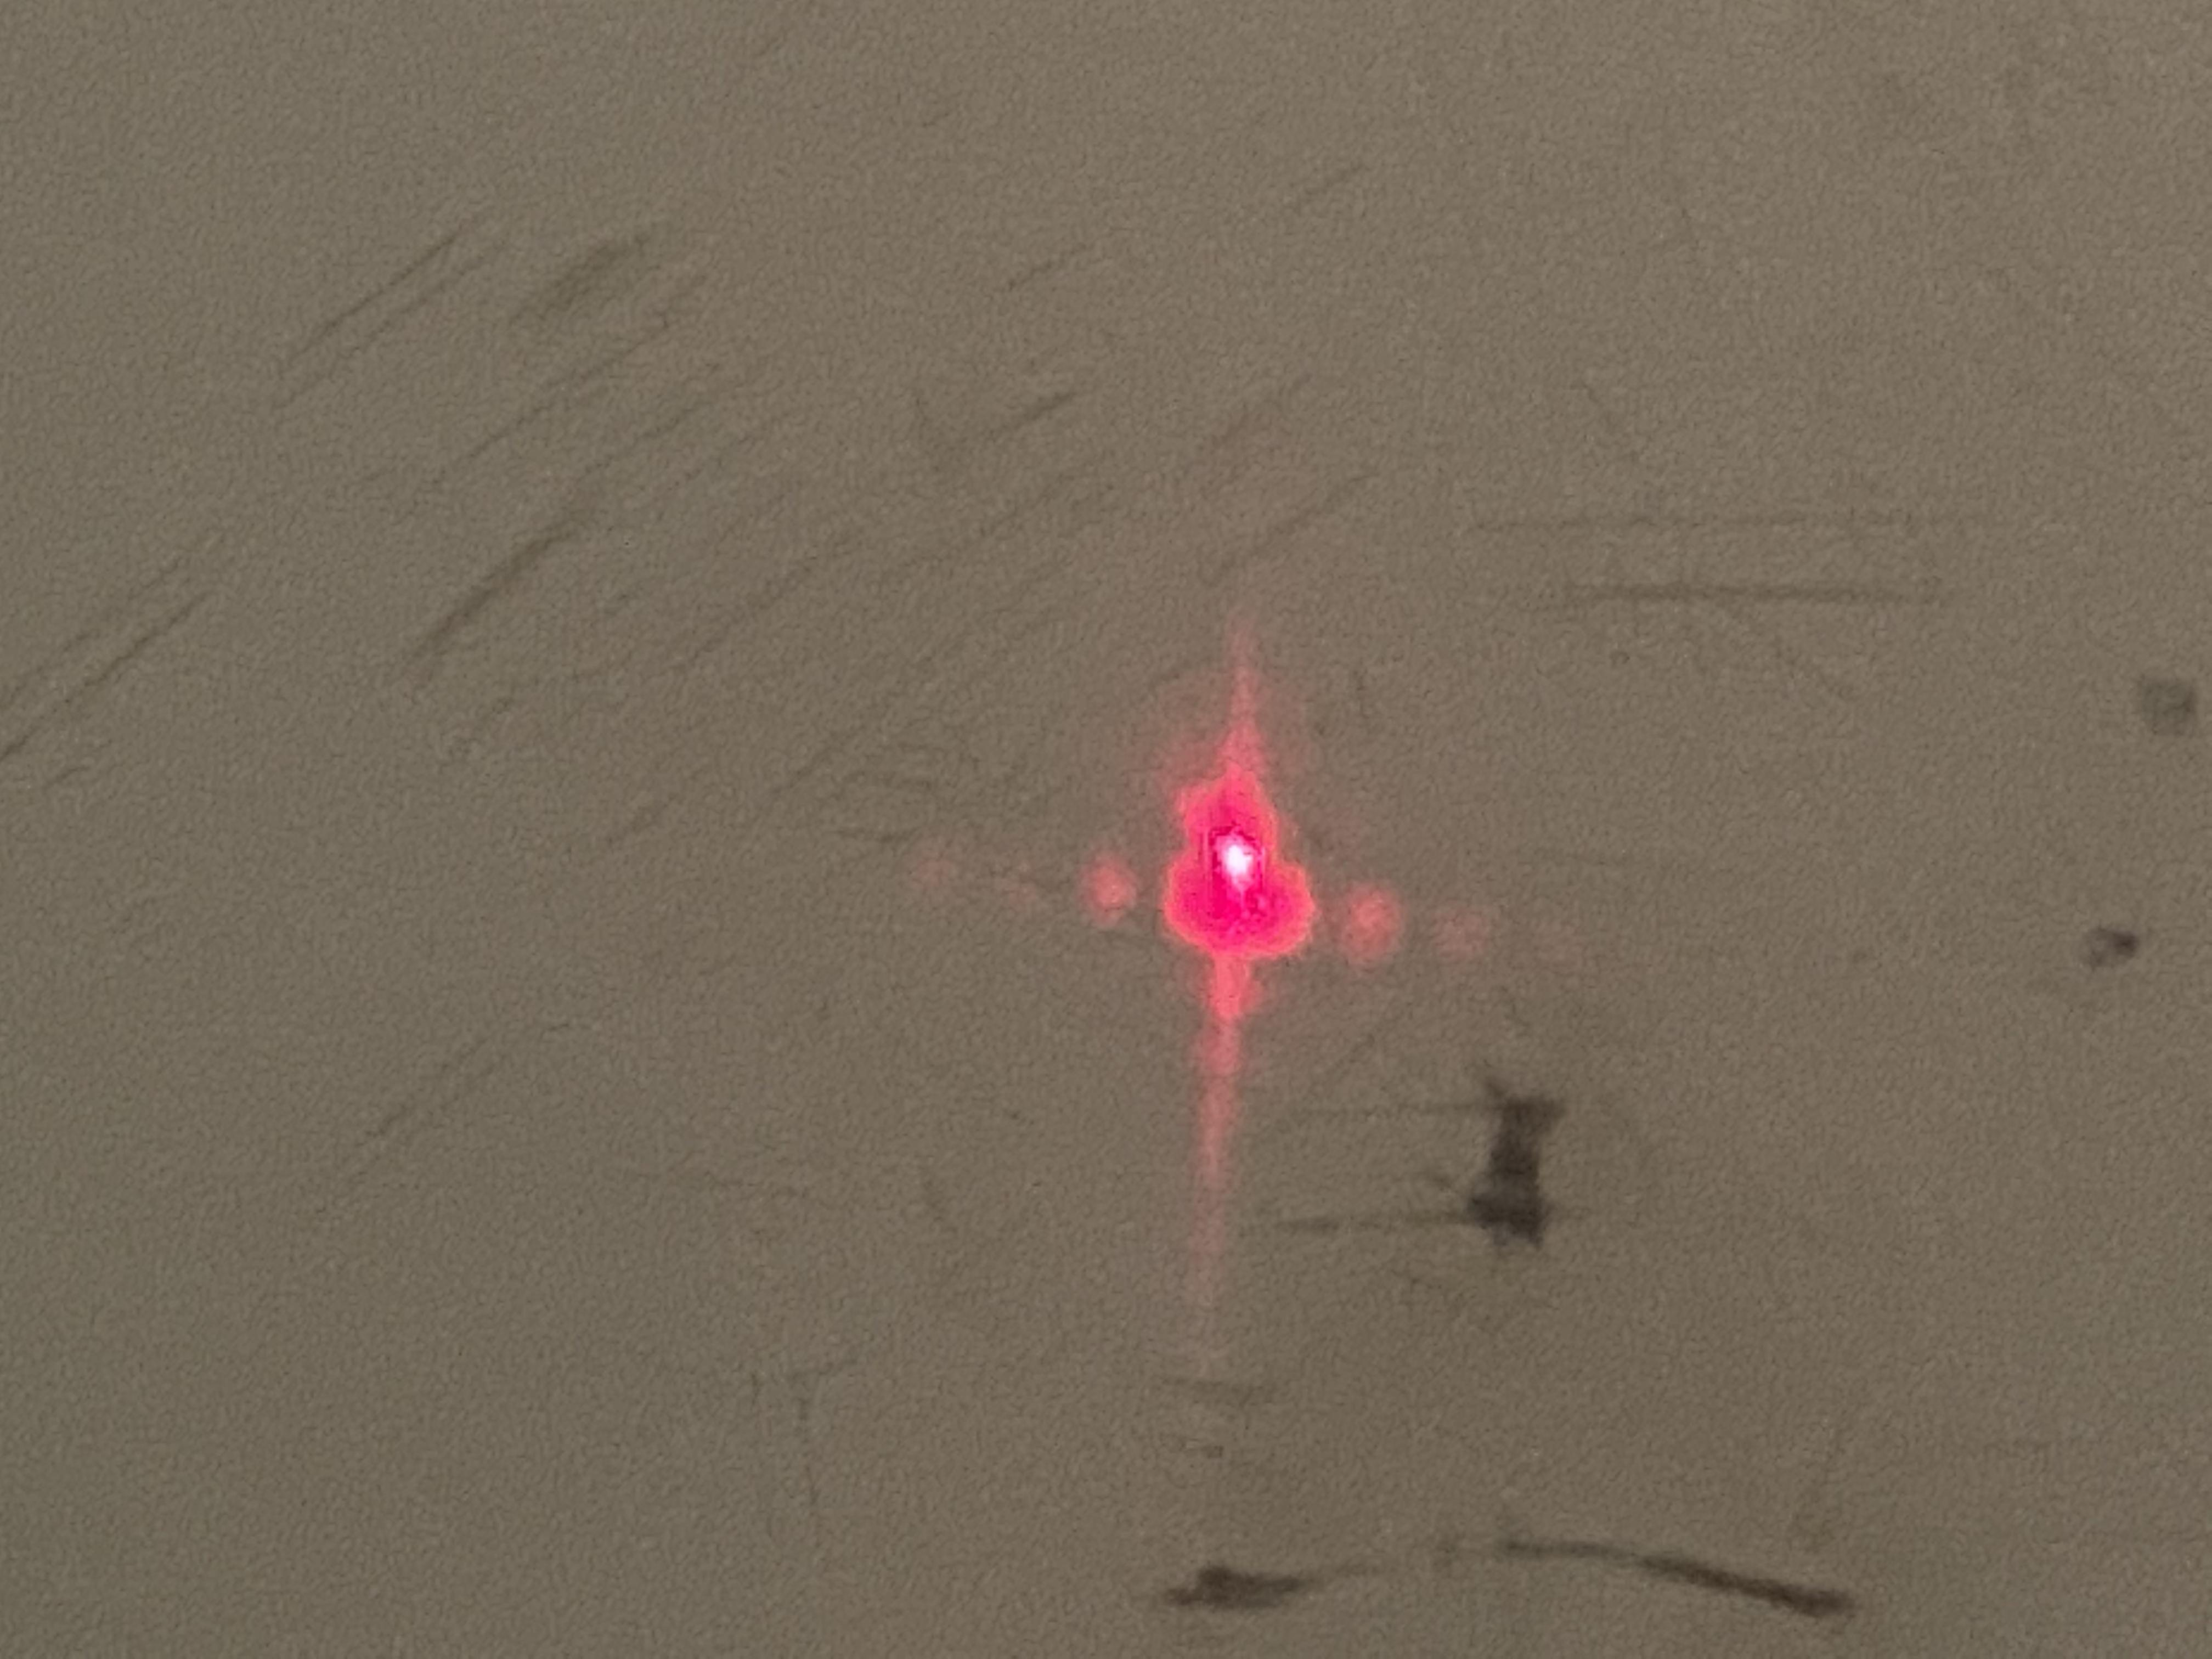
\includegraphics[height=5cm]{./pictures/photos/分划板2_矩孔.jpg}
    \caption{分划板2 矩孔}
    \label{fig:分划板2_矩孔}
  \end{subfigure}
  \label{fig:combined}
\end{figure}

\begin{figure}[H]
  \centering
  \begin{subfigure}[b]{0.45\textwidth}
    \centering
    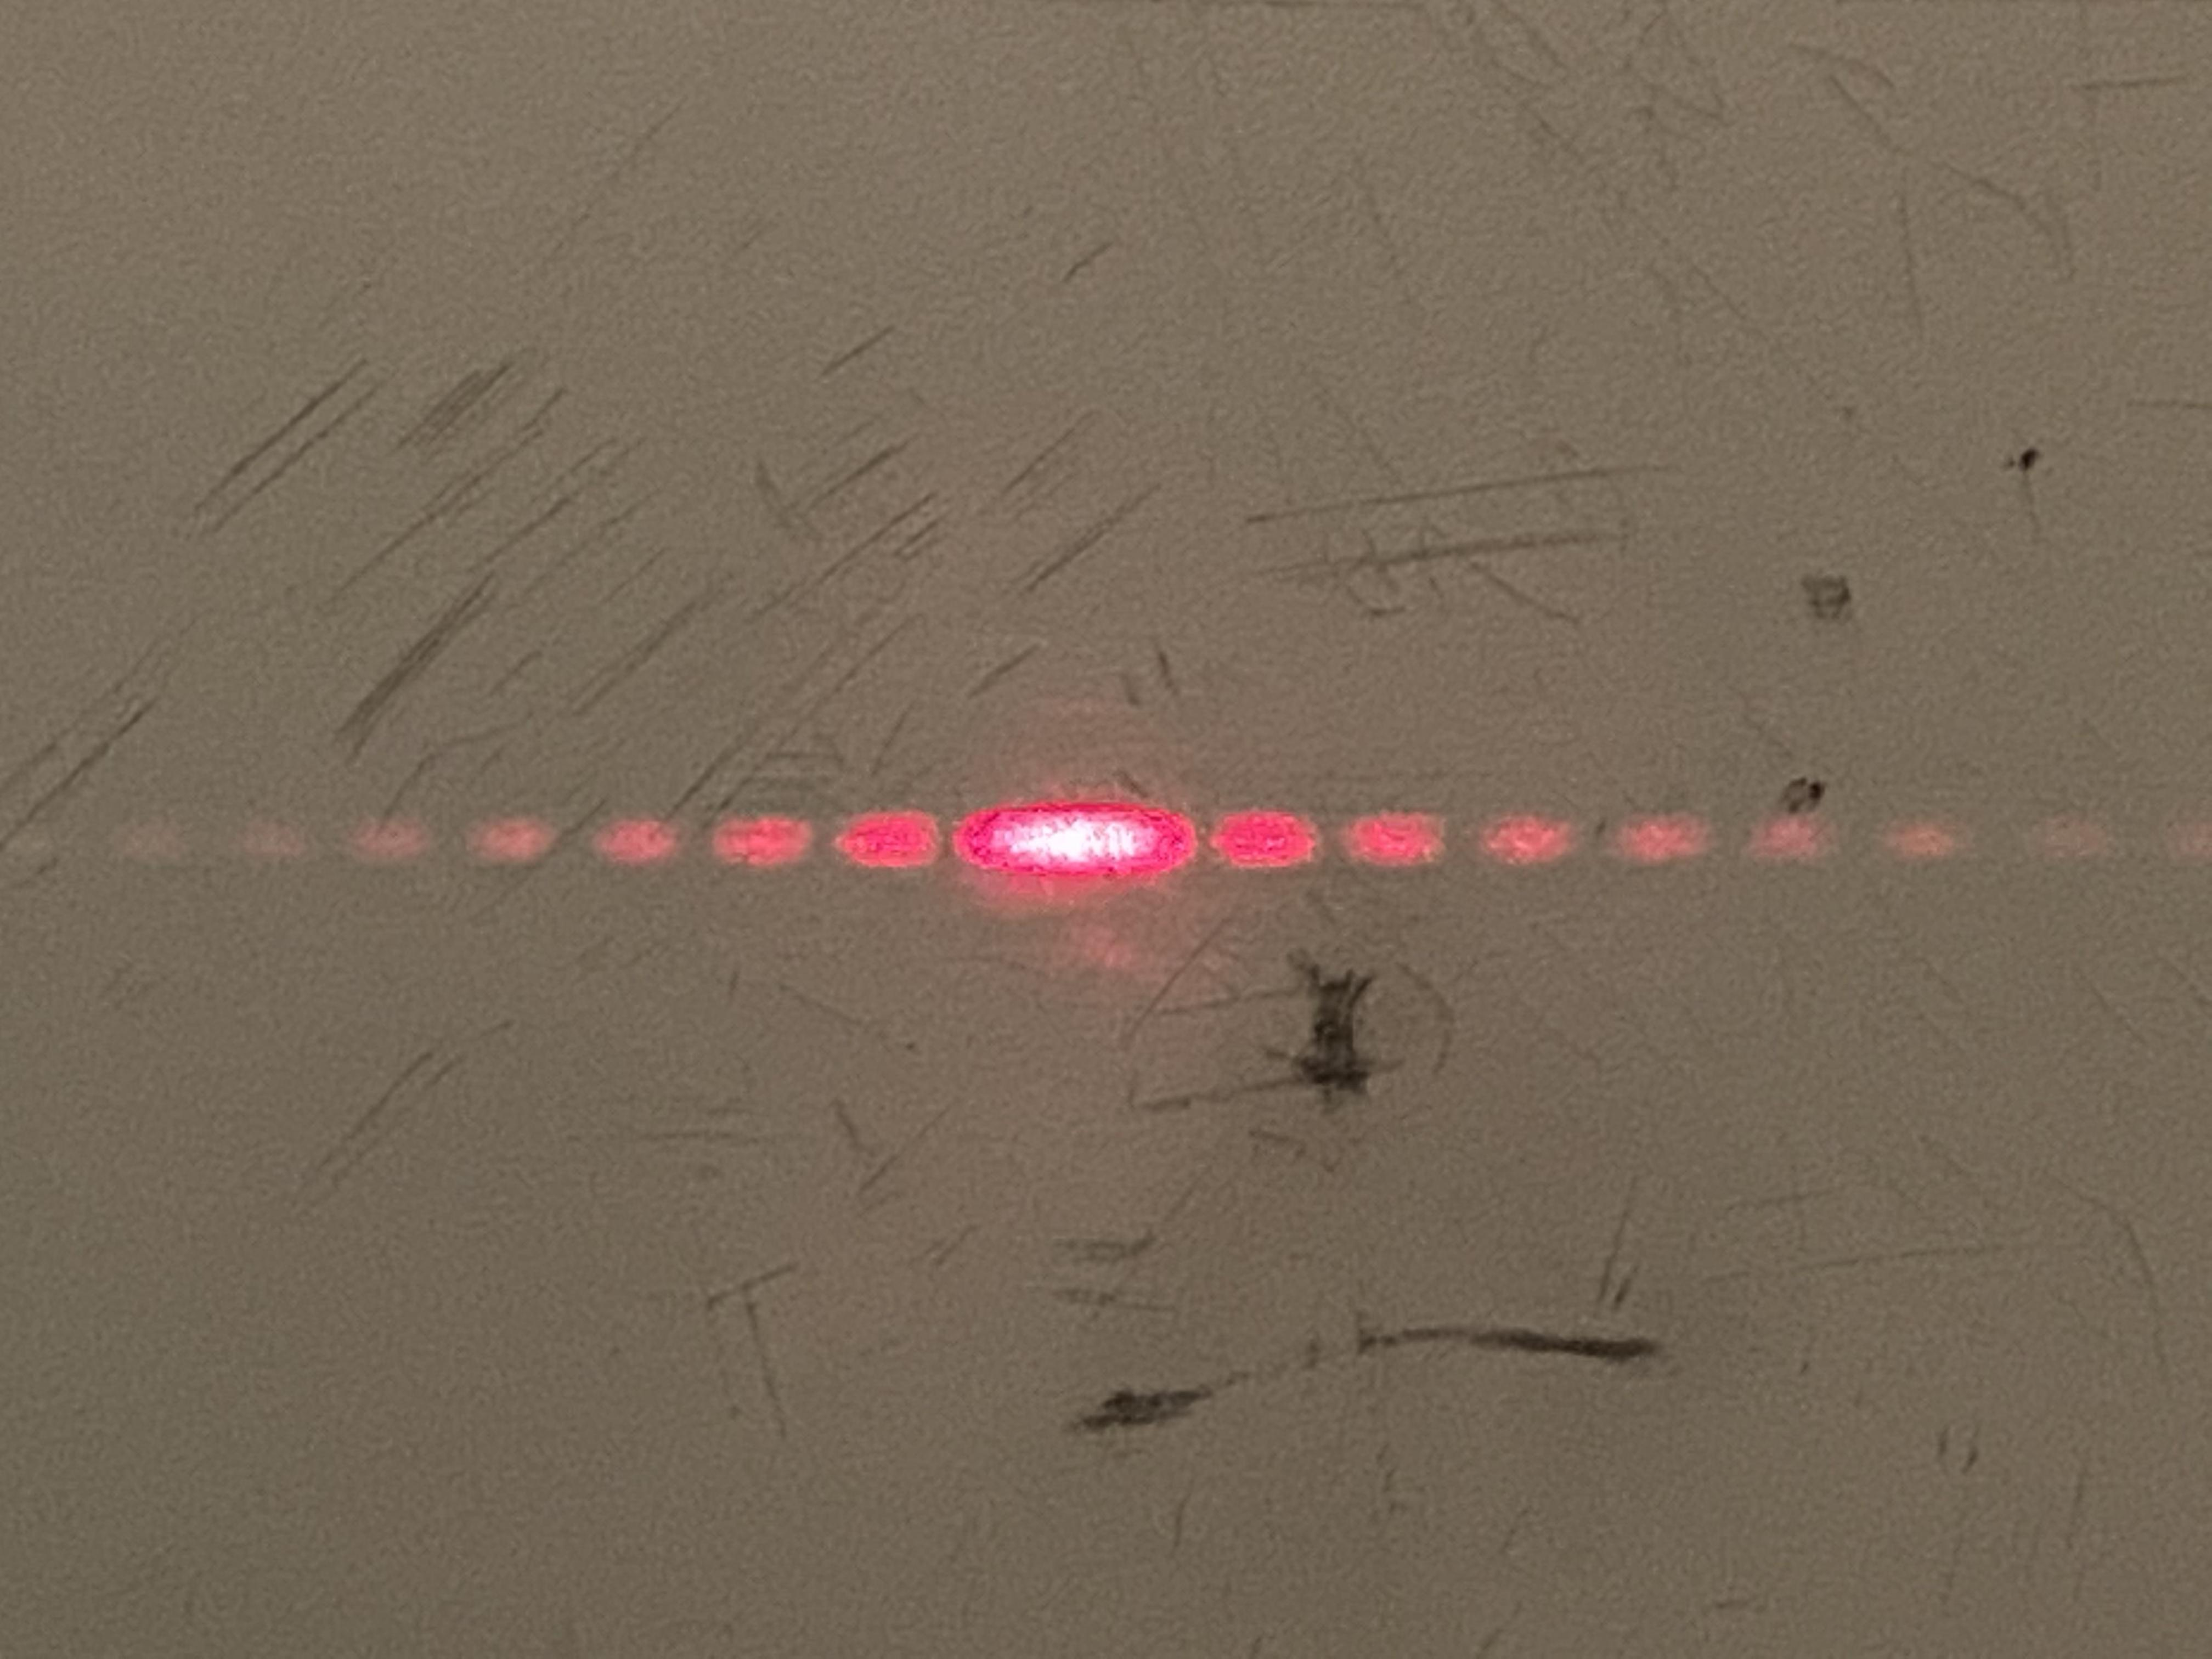
\includegraphics[height=5cm]{./pictures/photos/分划板2_单缝.jpg}
    \caption{分划板2 单缝}
    \label{fig:分划板2_单缝}
  \end{subfigure}
  \hfill
  \begin{subfigure}[b]{0.45\textwidth}
    \centering
    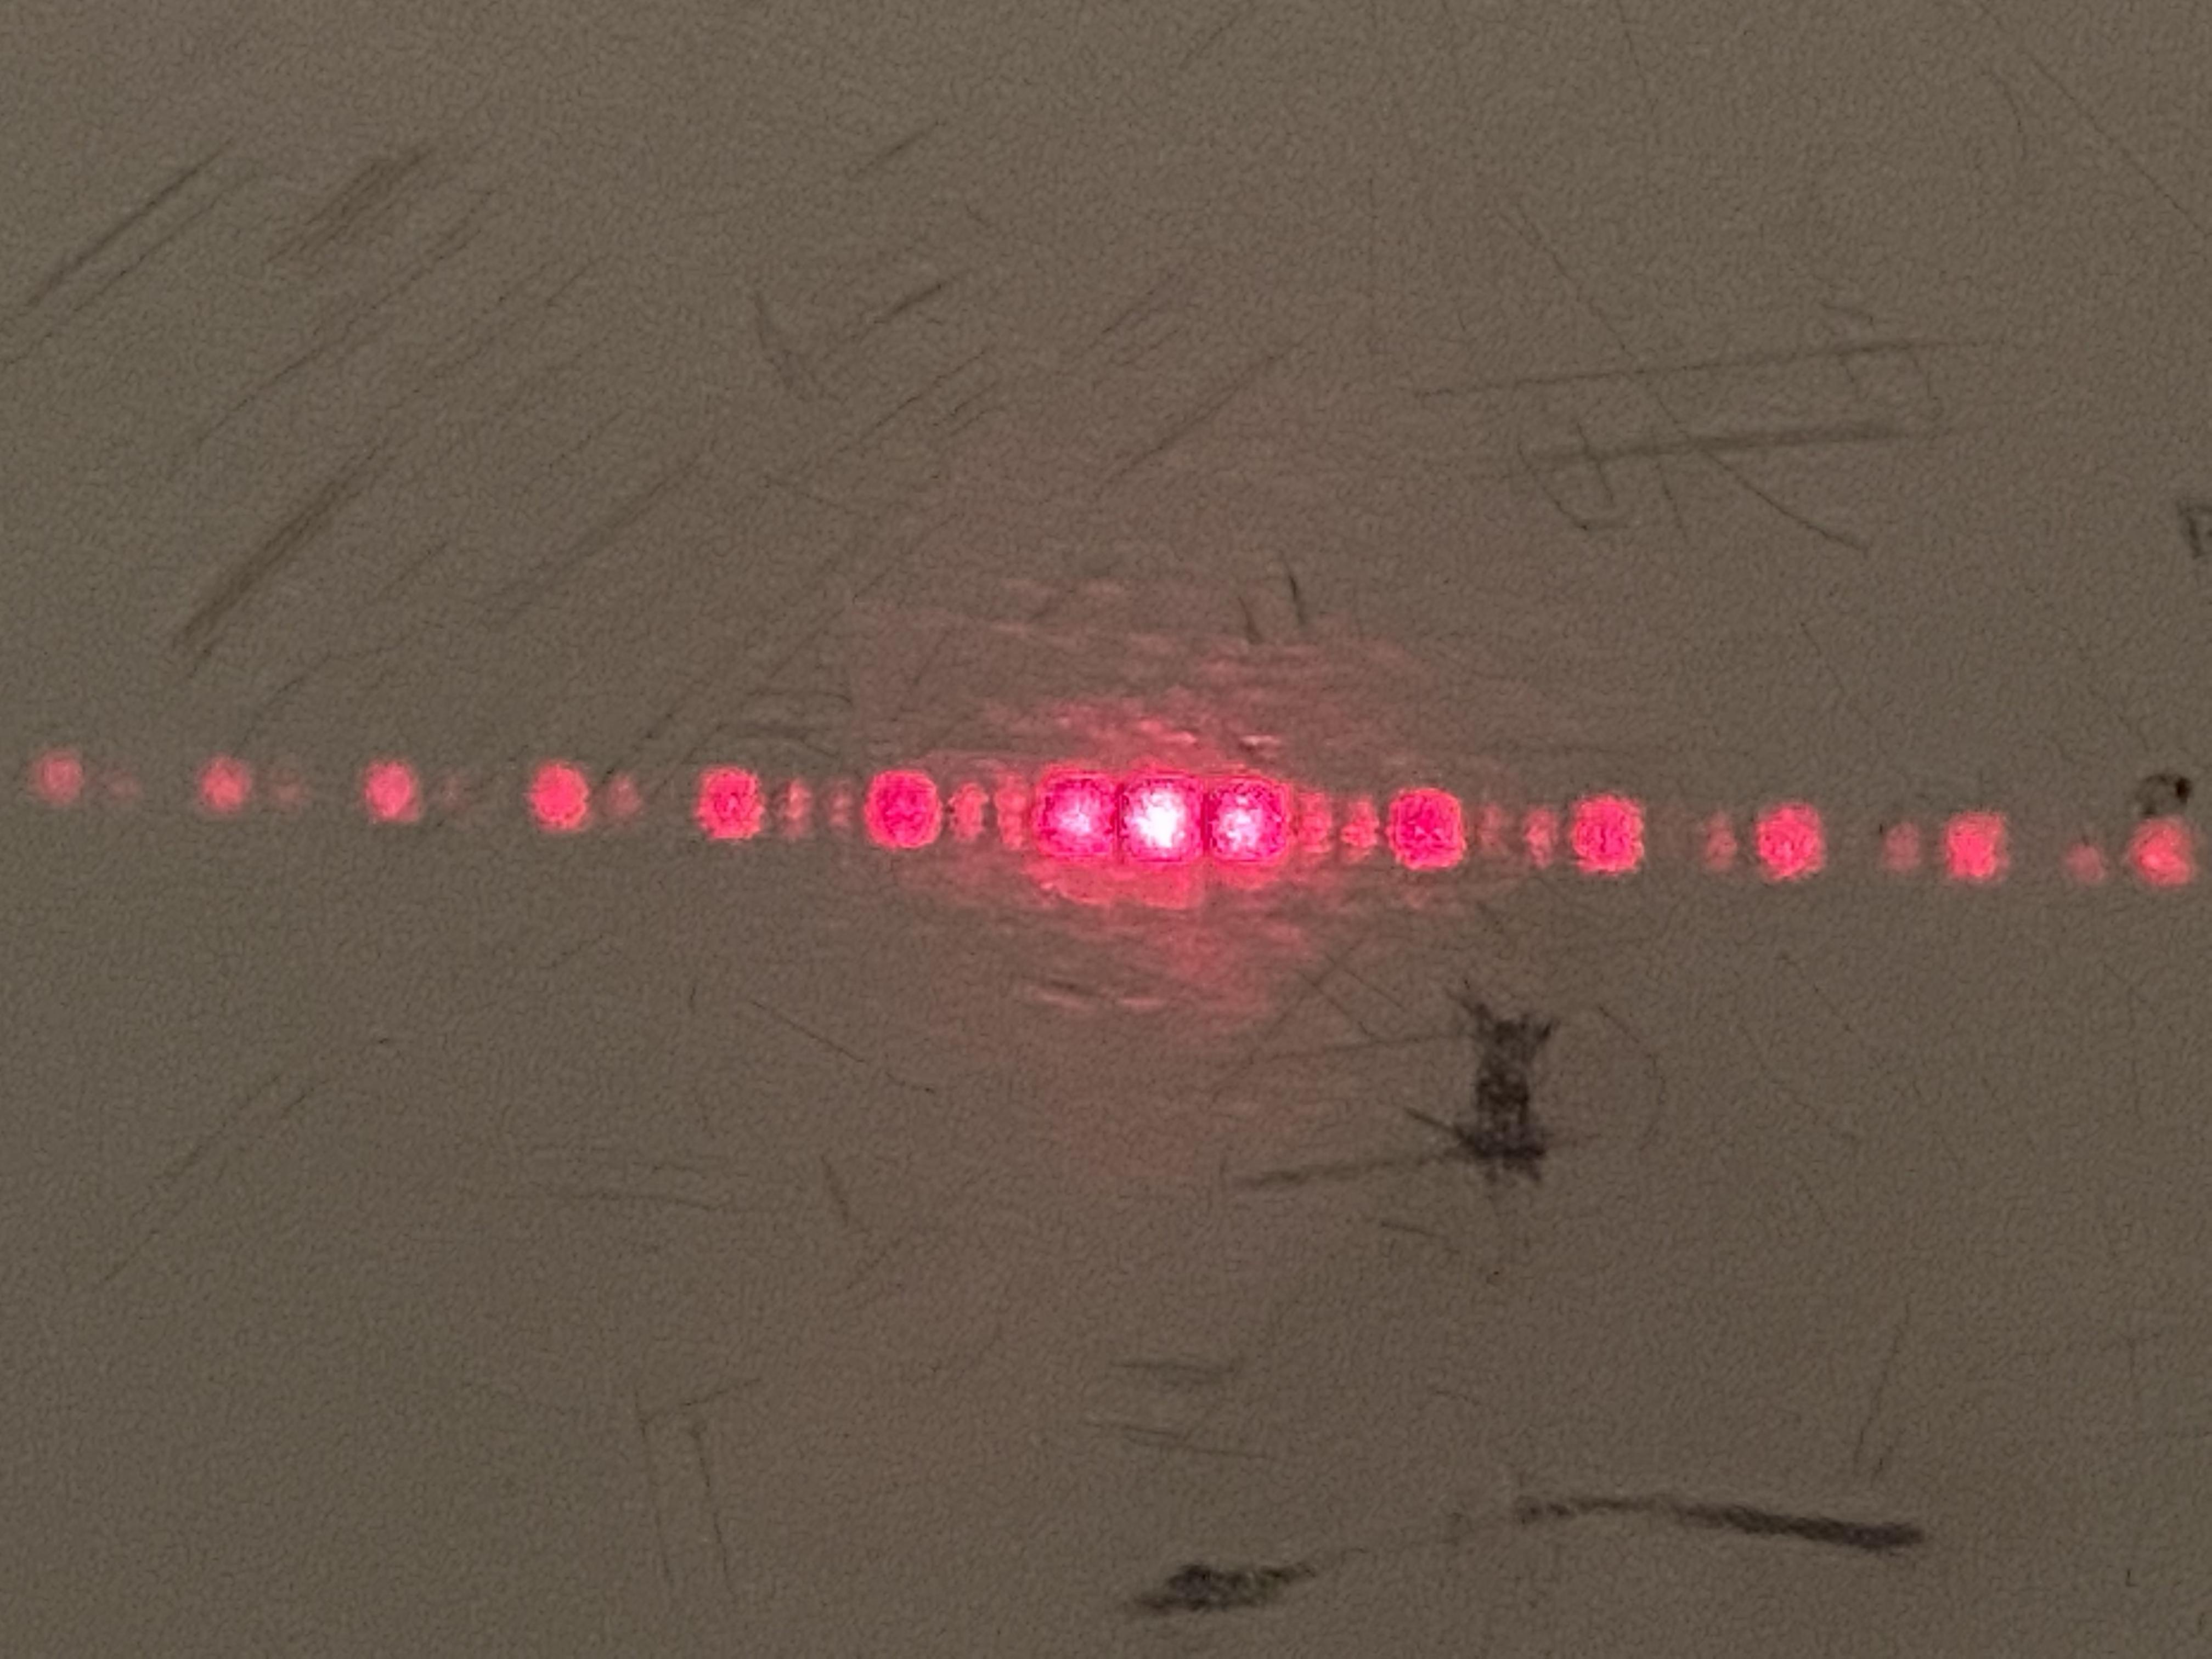
\includegraphics[height=5cm]{./pictures/photos/分划板2_双缝1.jpg}
    \caption{分划板2 双缝1}
    \label{fig:分划板2_双缝1}
  \end{subfigure}
  \label{fig:combined}
\end{figure}

\begin{figure}[H]
  \centering
  \begin{subfigure}[b]{0.45\textwidth}
    \centering
    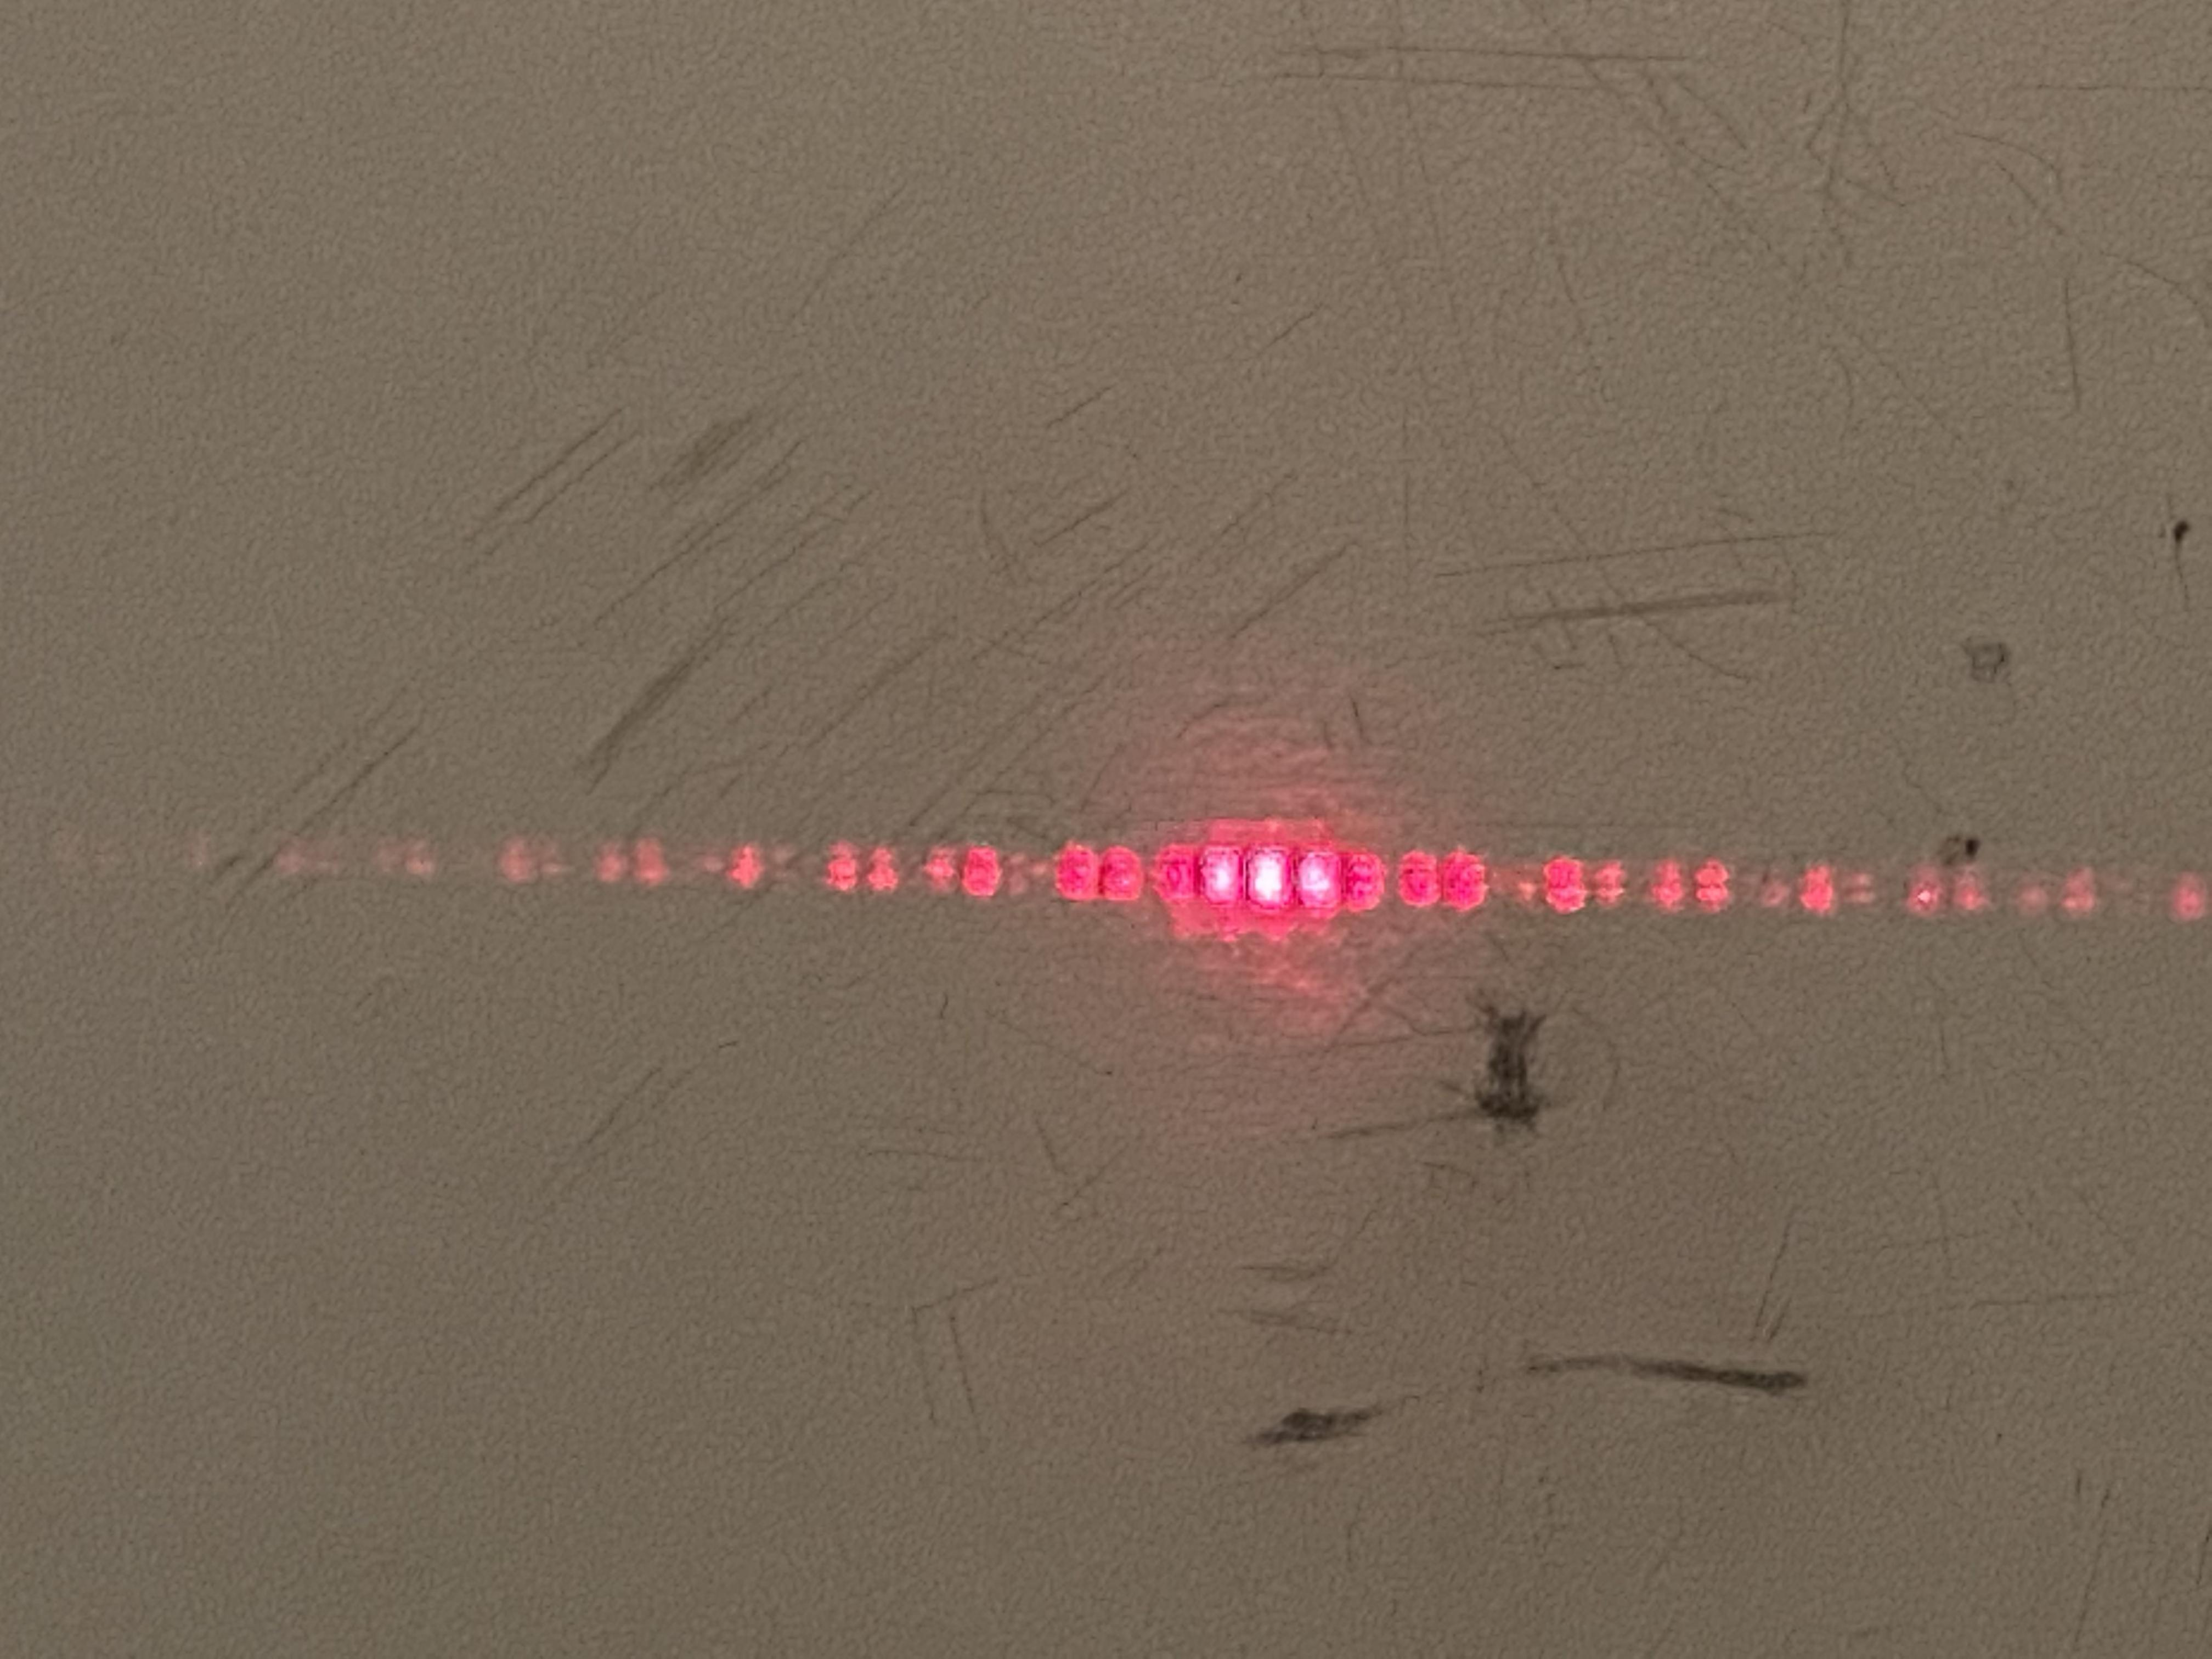
\includegraphics[height=5cm]{./pictures/photos/分划板2_双缝2.jpg}
    \caption{分划板2 双缝2}
    \label{fig:分划板2_双缝2}      
  \end{subfigure}
  \hfill
  \begin{subfigure}[b]{0.45\textwidth}
    \centering
    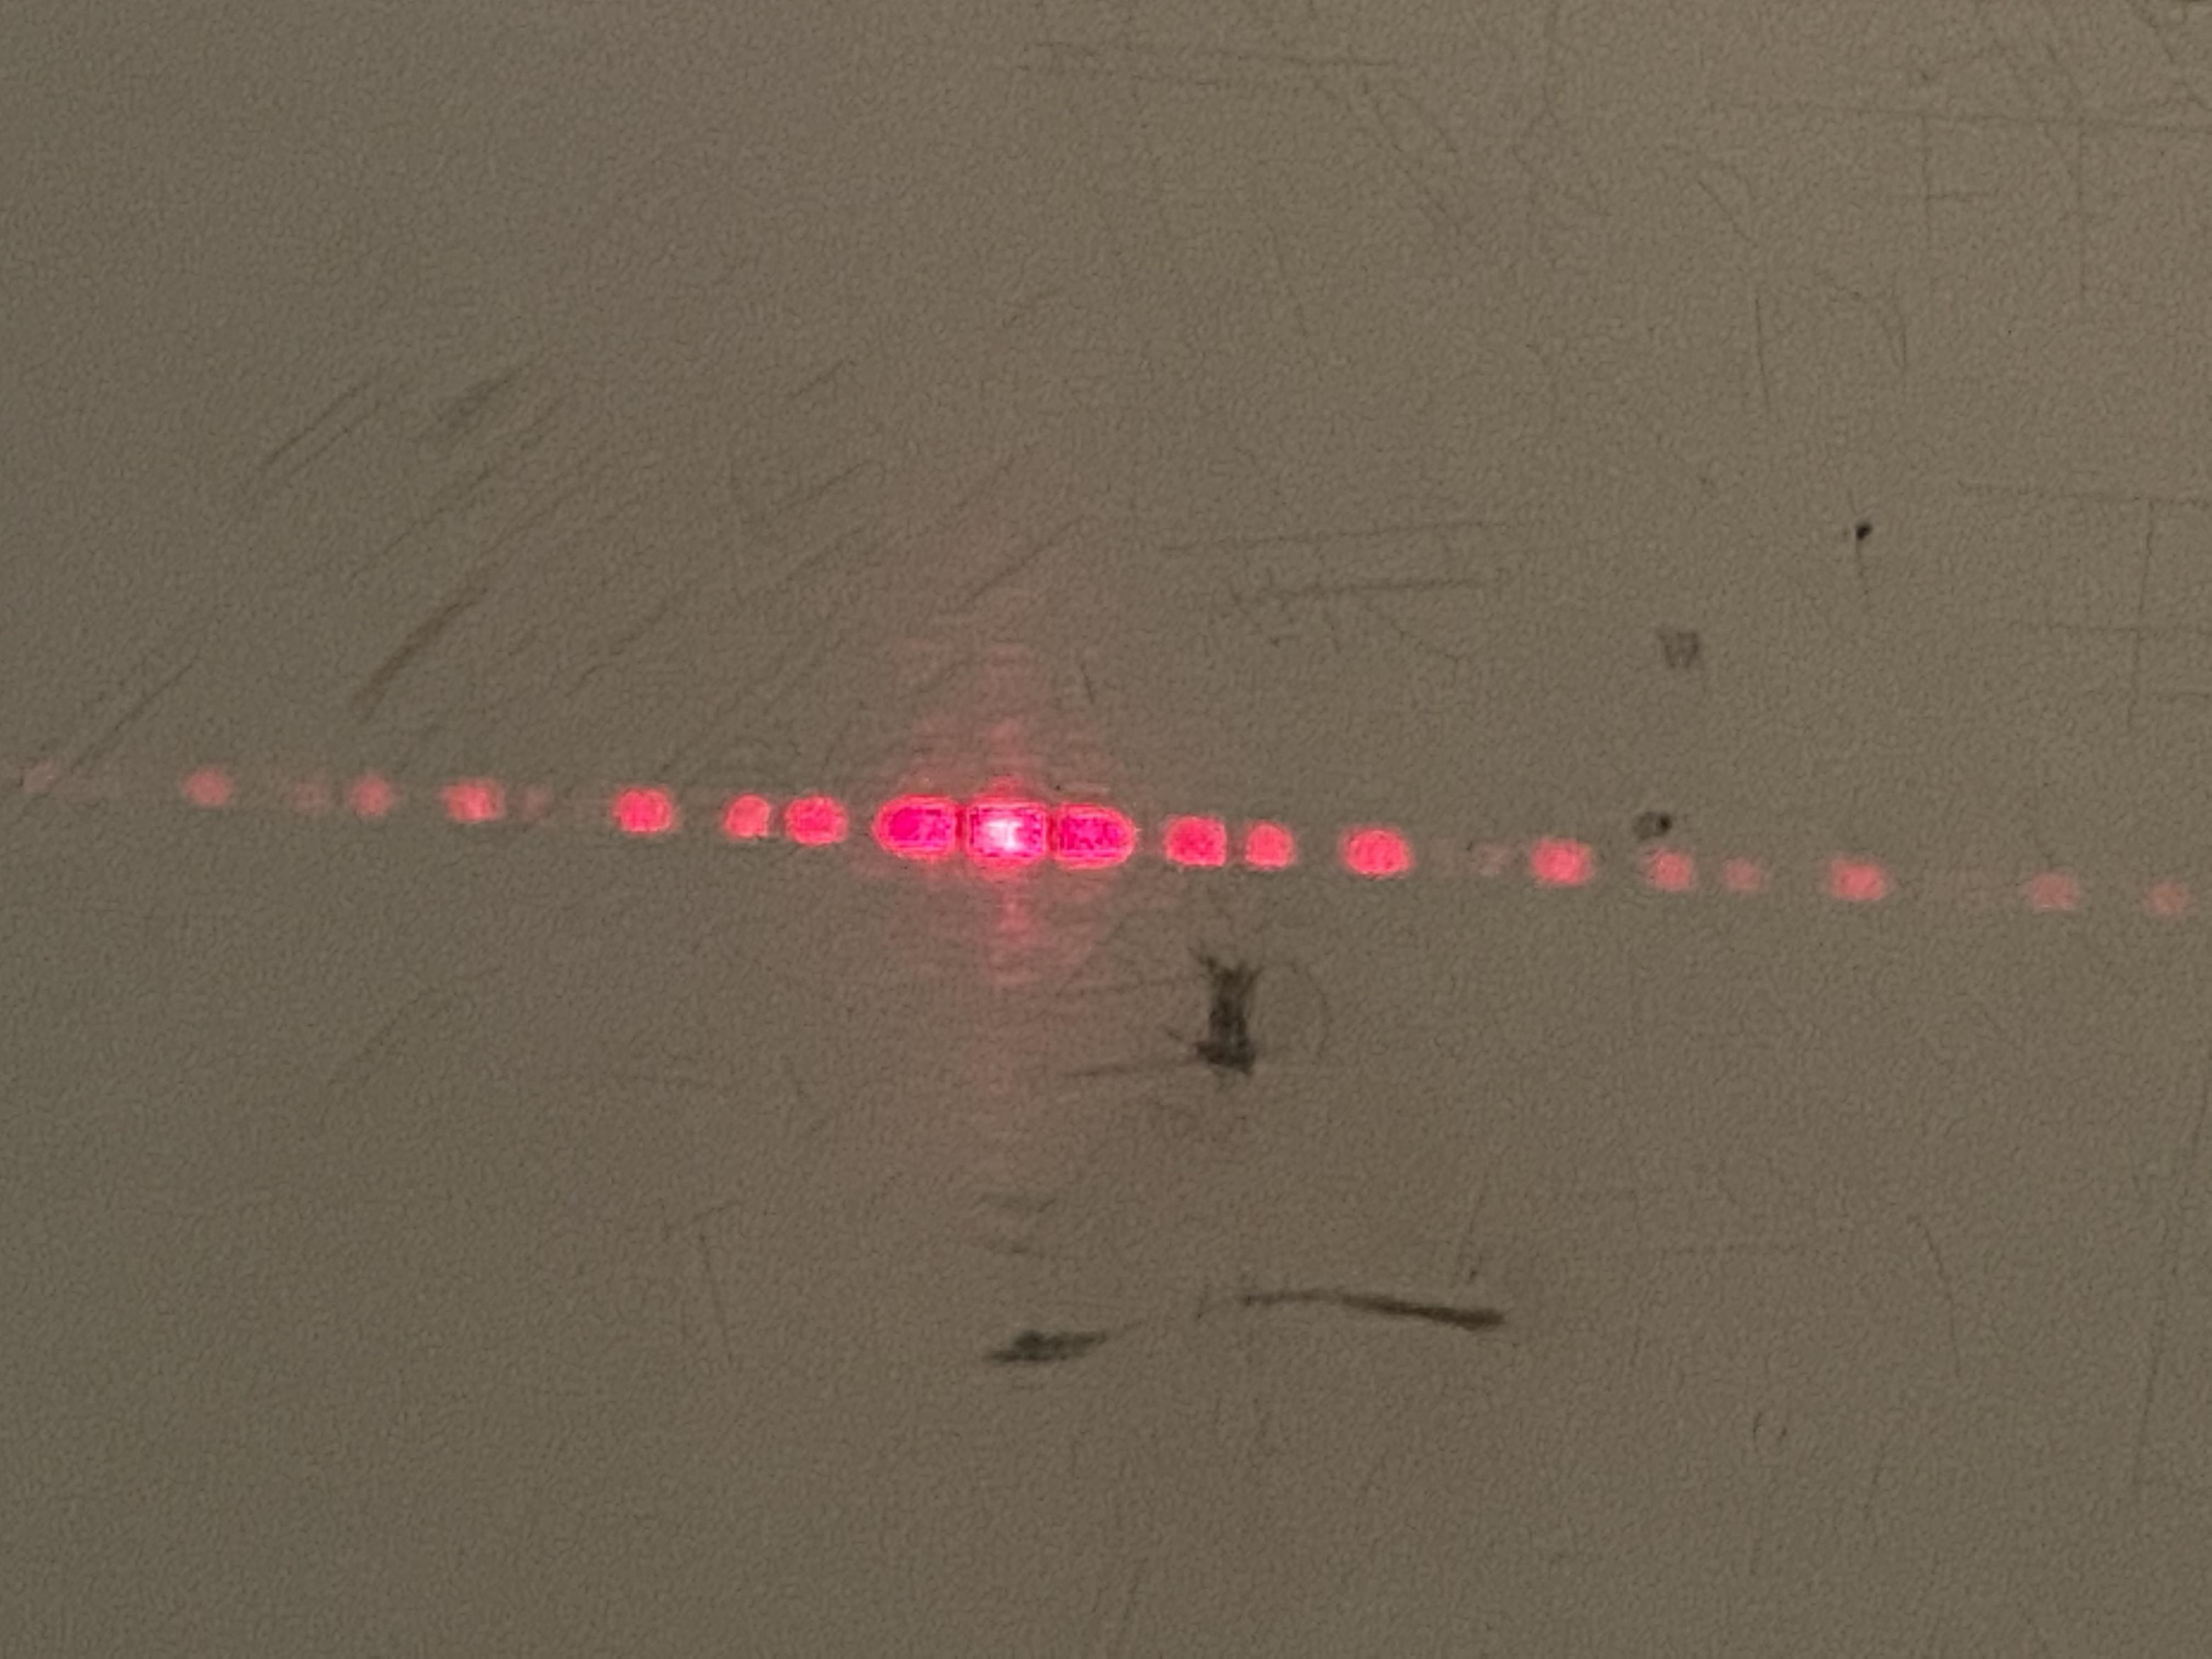
\includegraphics[height=5cm]{./pictures/photos/分划板2_双缝3.jpg}
    \caption{分划板2 双缝3}
    \label{fig:分划板2_双缝3}
  \end{subfigure}
  \label{fig:combined}
\end{figure}

\begin{figure}[H]
  \centering
  \begin{subfigure}[b]{0.45\textwidth}
    \centering
    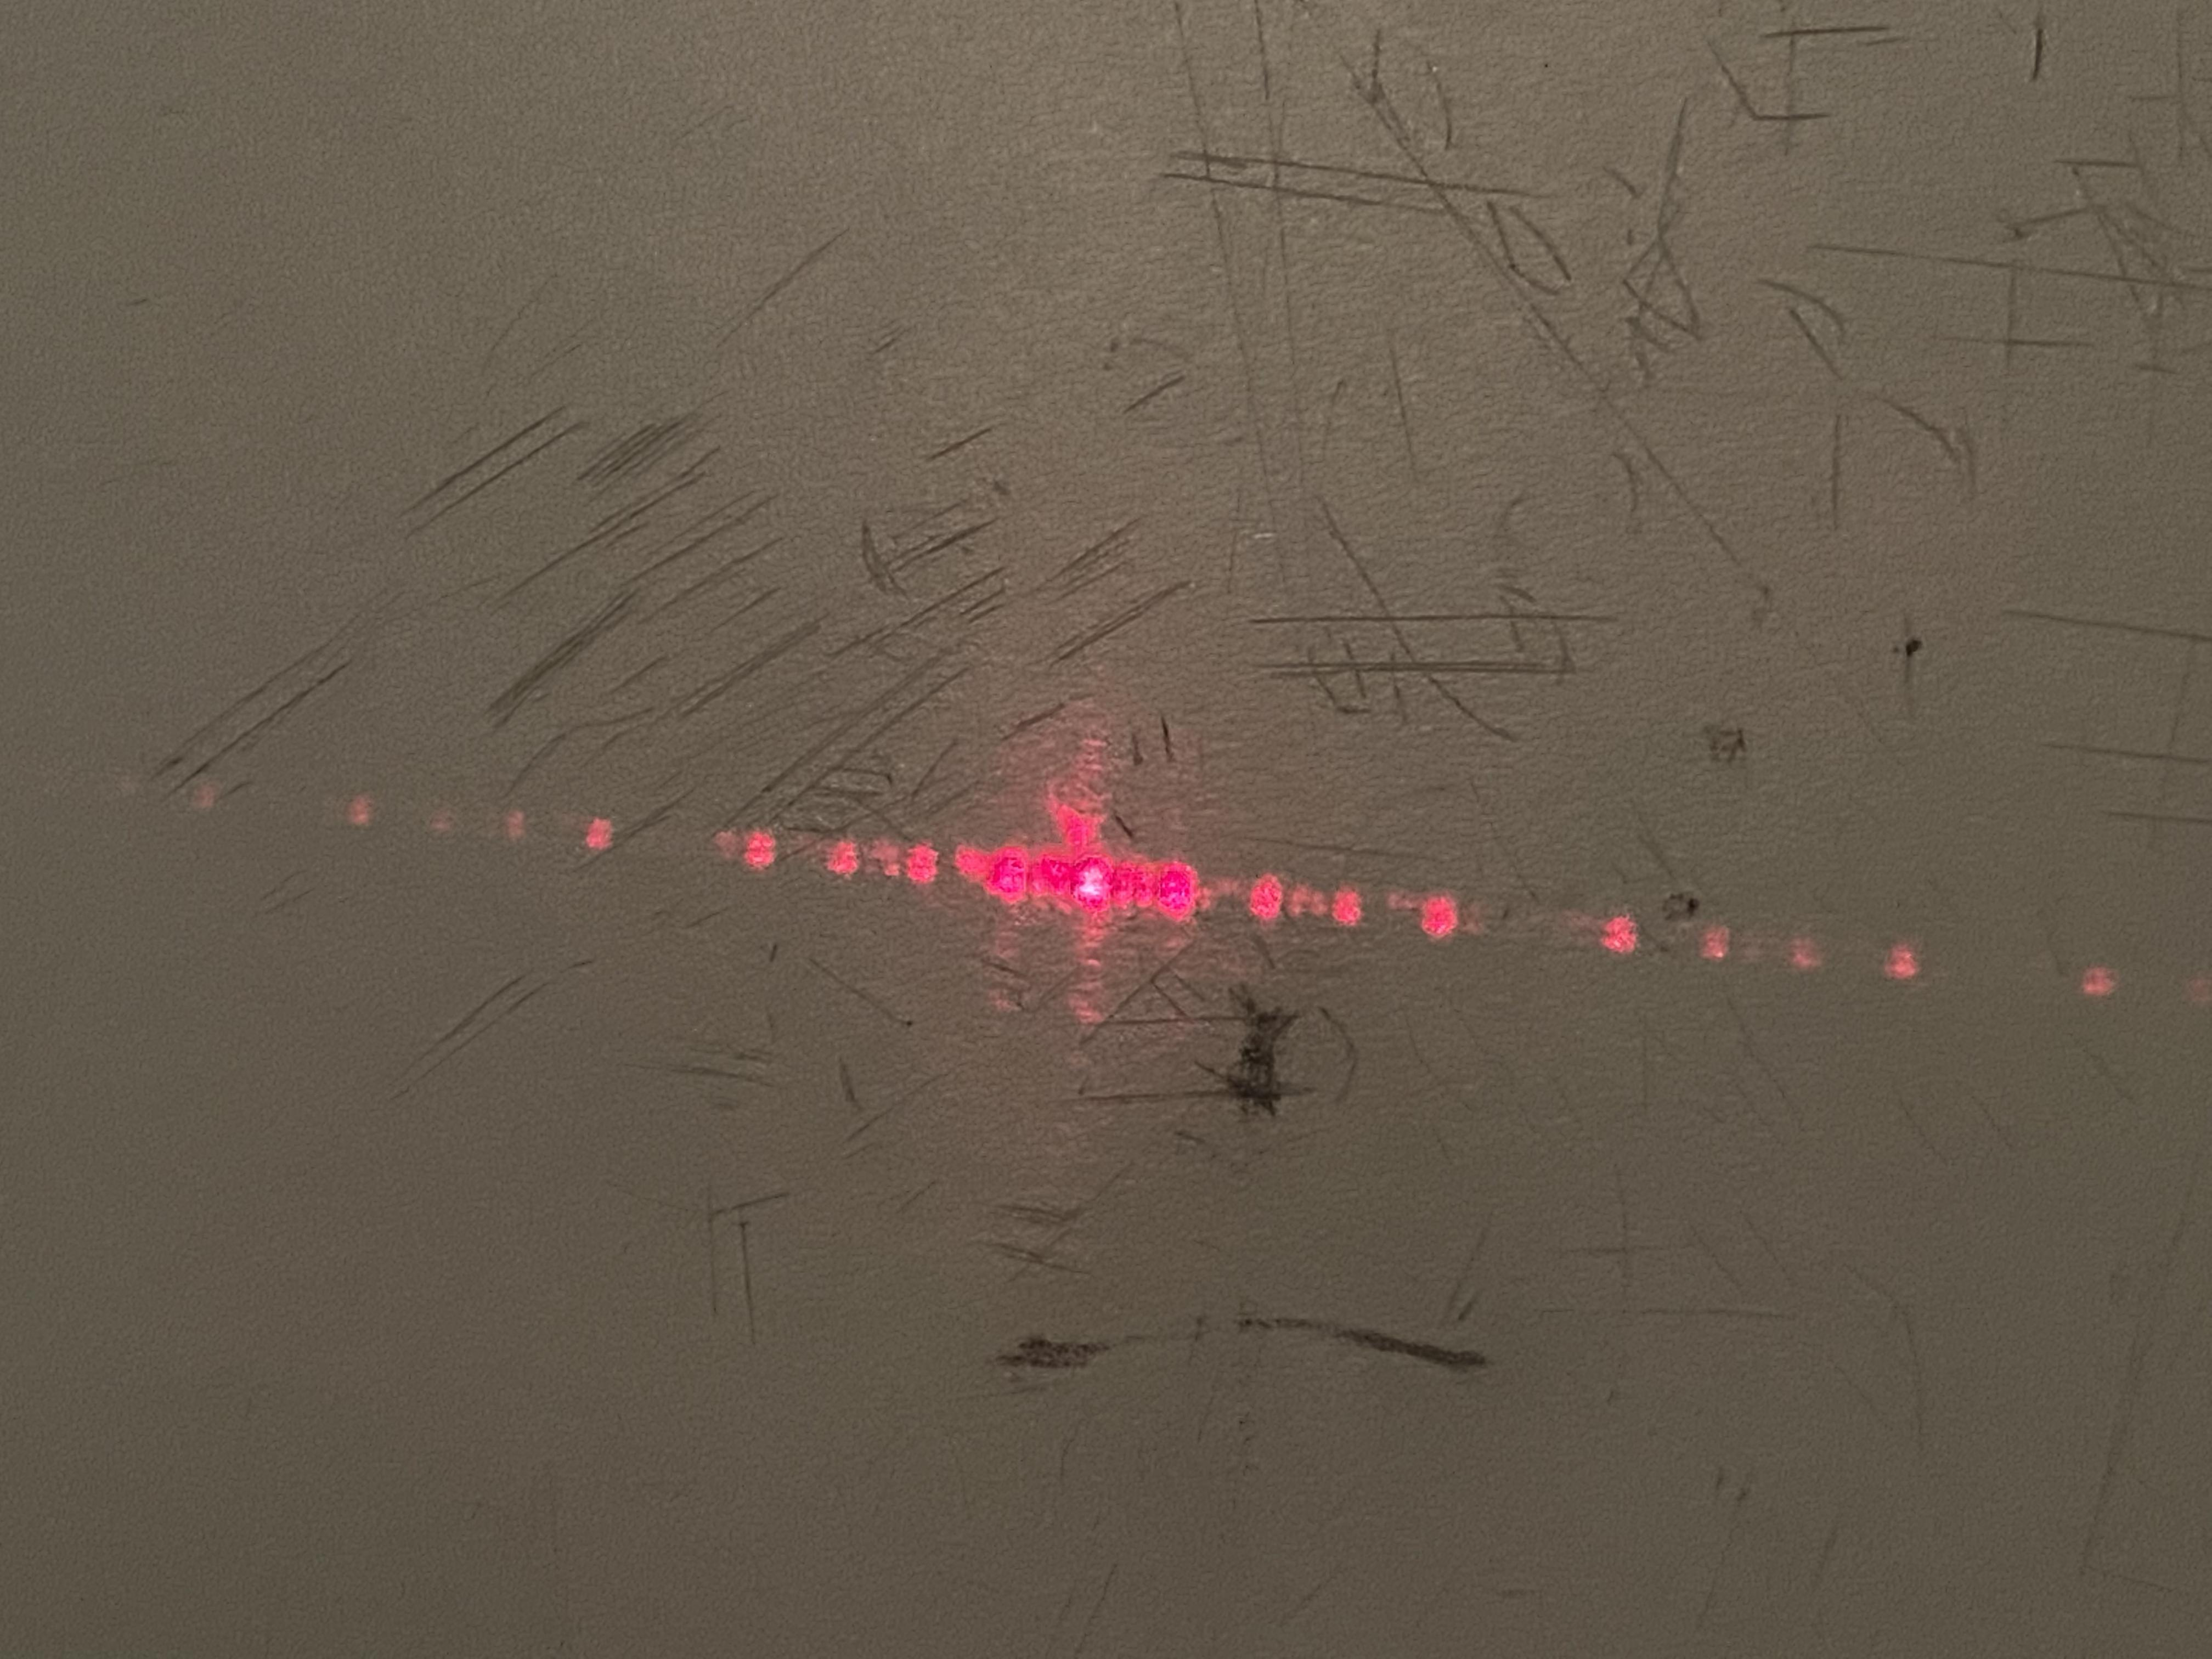
\includegraphics[height=5cm]{./pictures/photos/分划板2_多缝1.jpg}
    \caption{分划板2 多缝1}
    \label{fig:分划板2_多缝1}
  \end{subfigure}
  \hfill
  \begin{subfigure}[b]{0.45\textwidth}
    \centering
    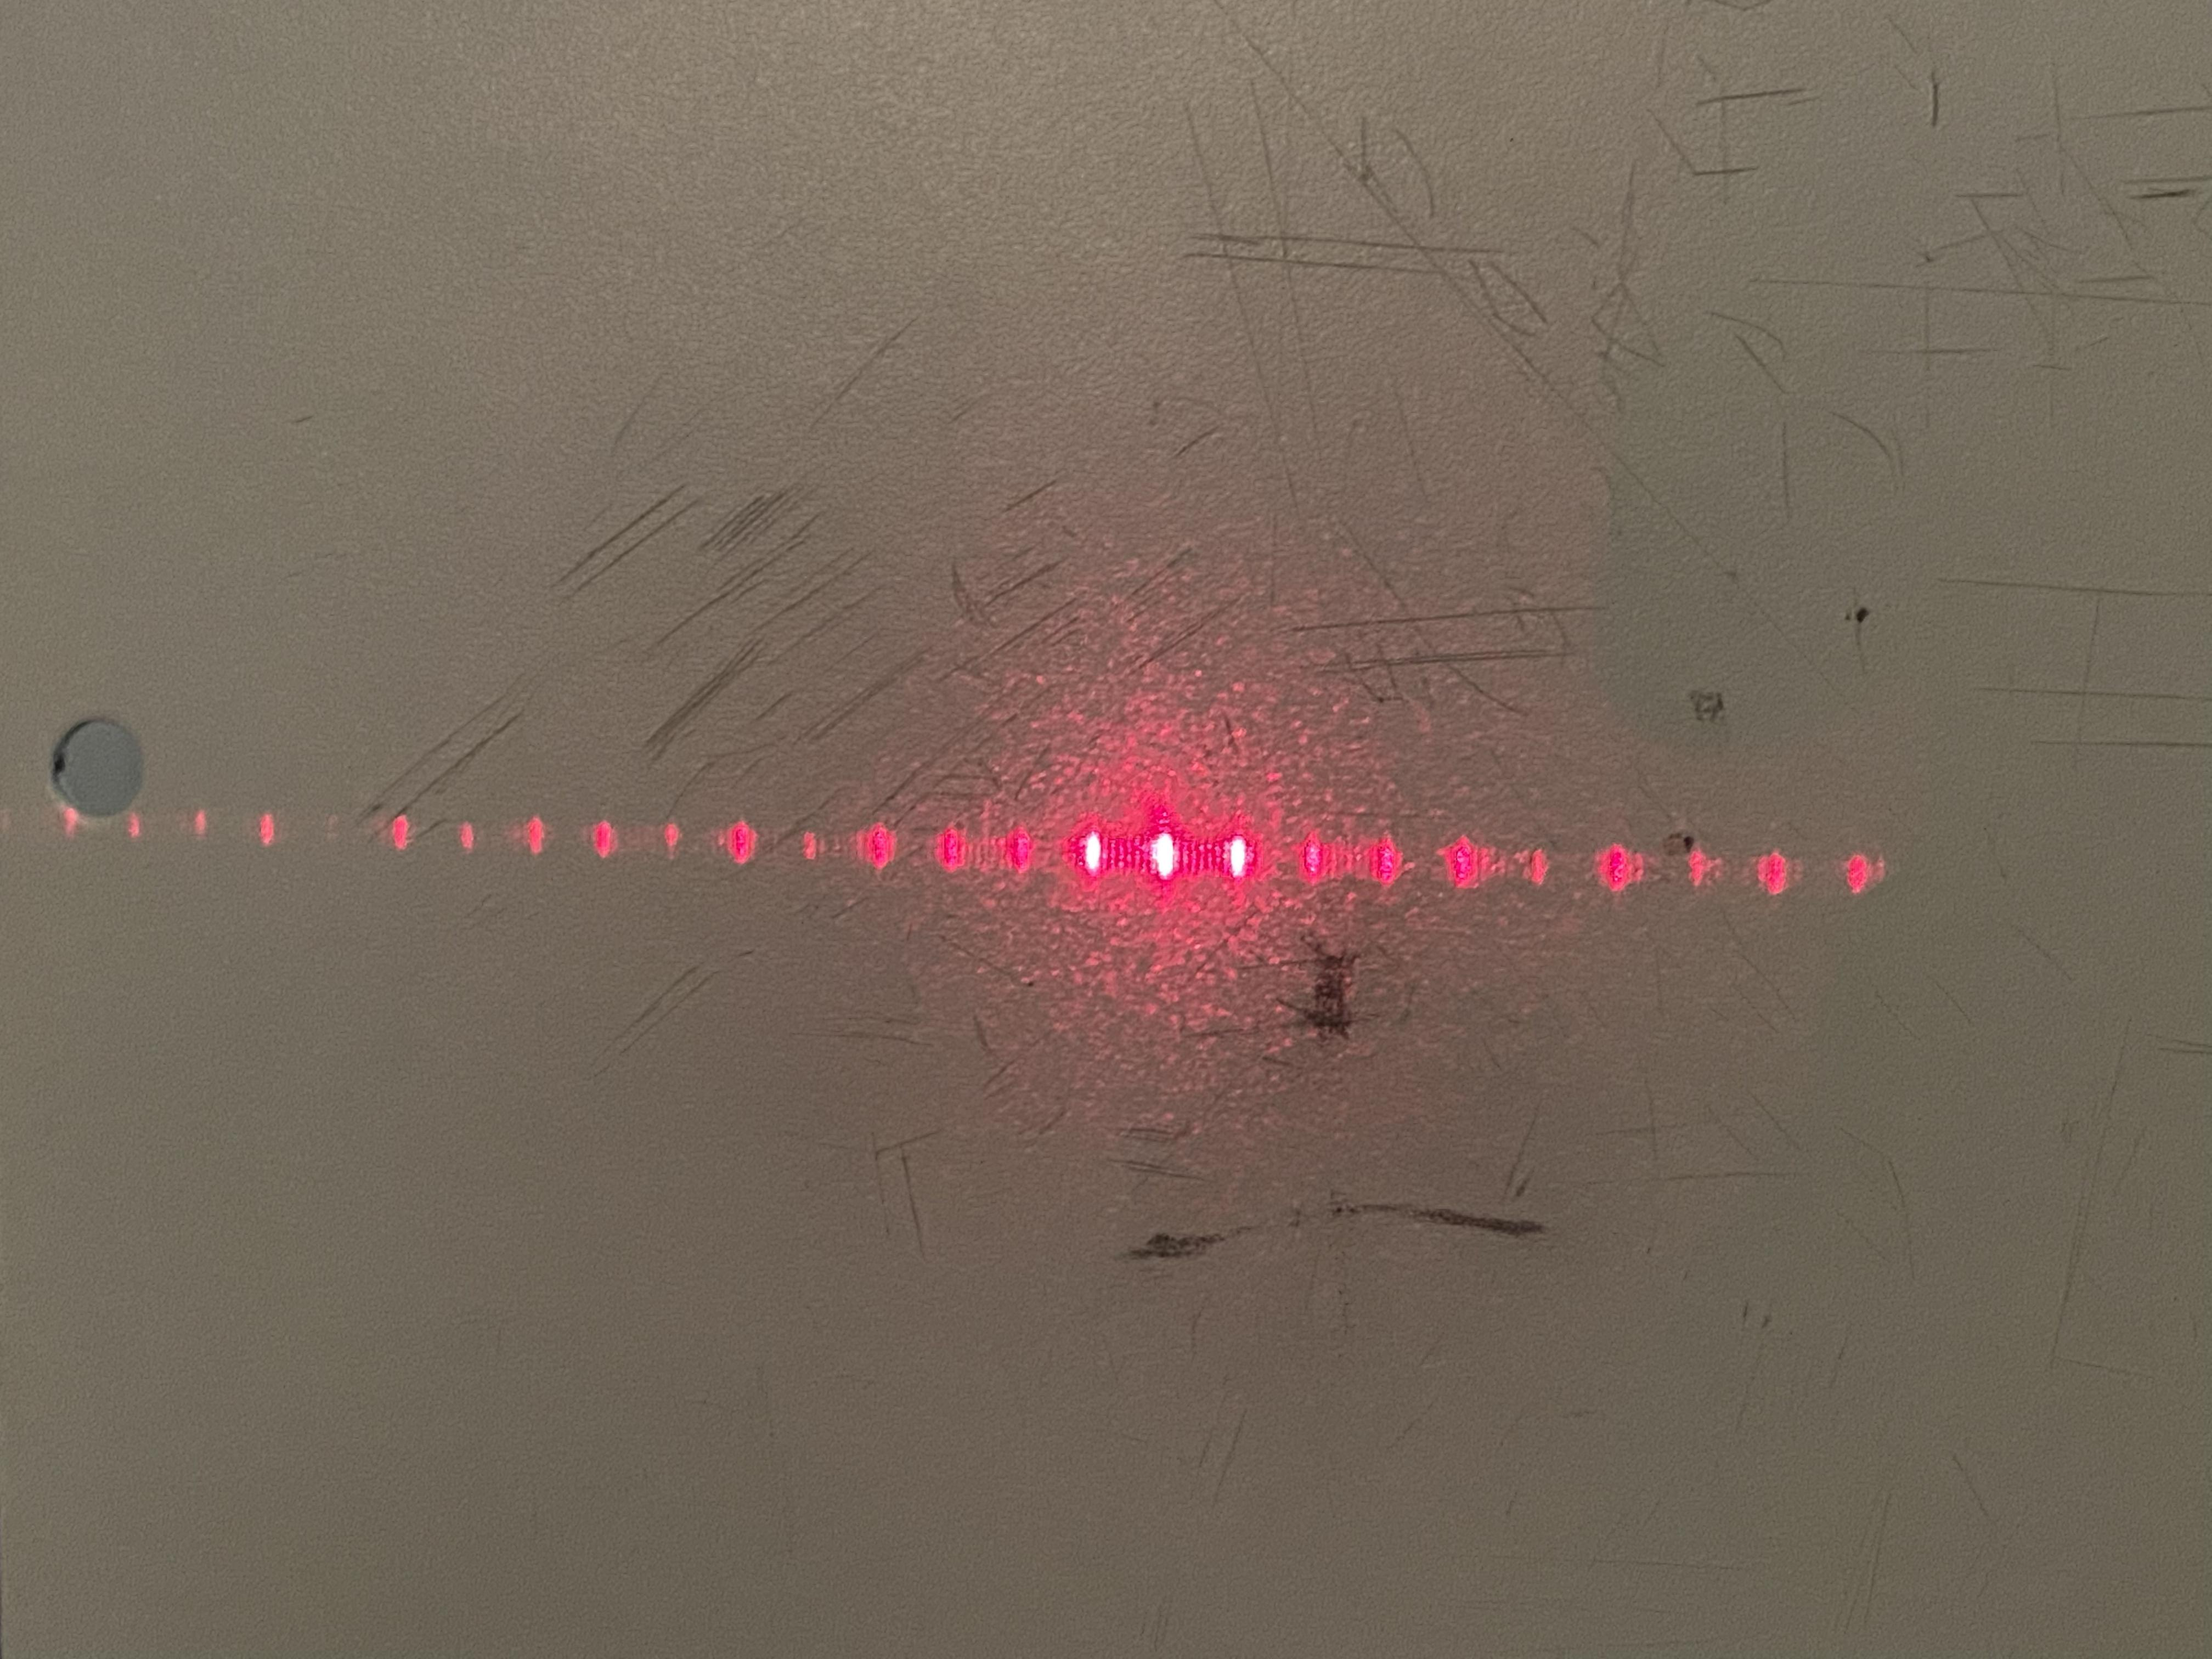
\includegraphics[height=5cm]{./pictures/photos/分划板2_多缝2.jpg}
    \caption{分划板2 多缝2}
    \label{fig:分划板2_多缝2}
  \end{subfigure}
  \label{fig:combined}
\end{figure}

\subsubsection{实验二：光栅衍射测量光栅常数实验}
\begin{figure}[H]
  \centering
  \begin{subfigure}[b]{0.45\textwidth}
    \centering
    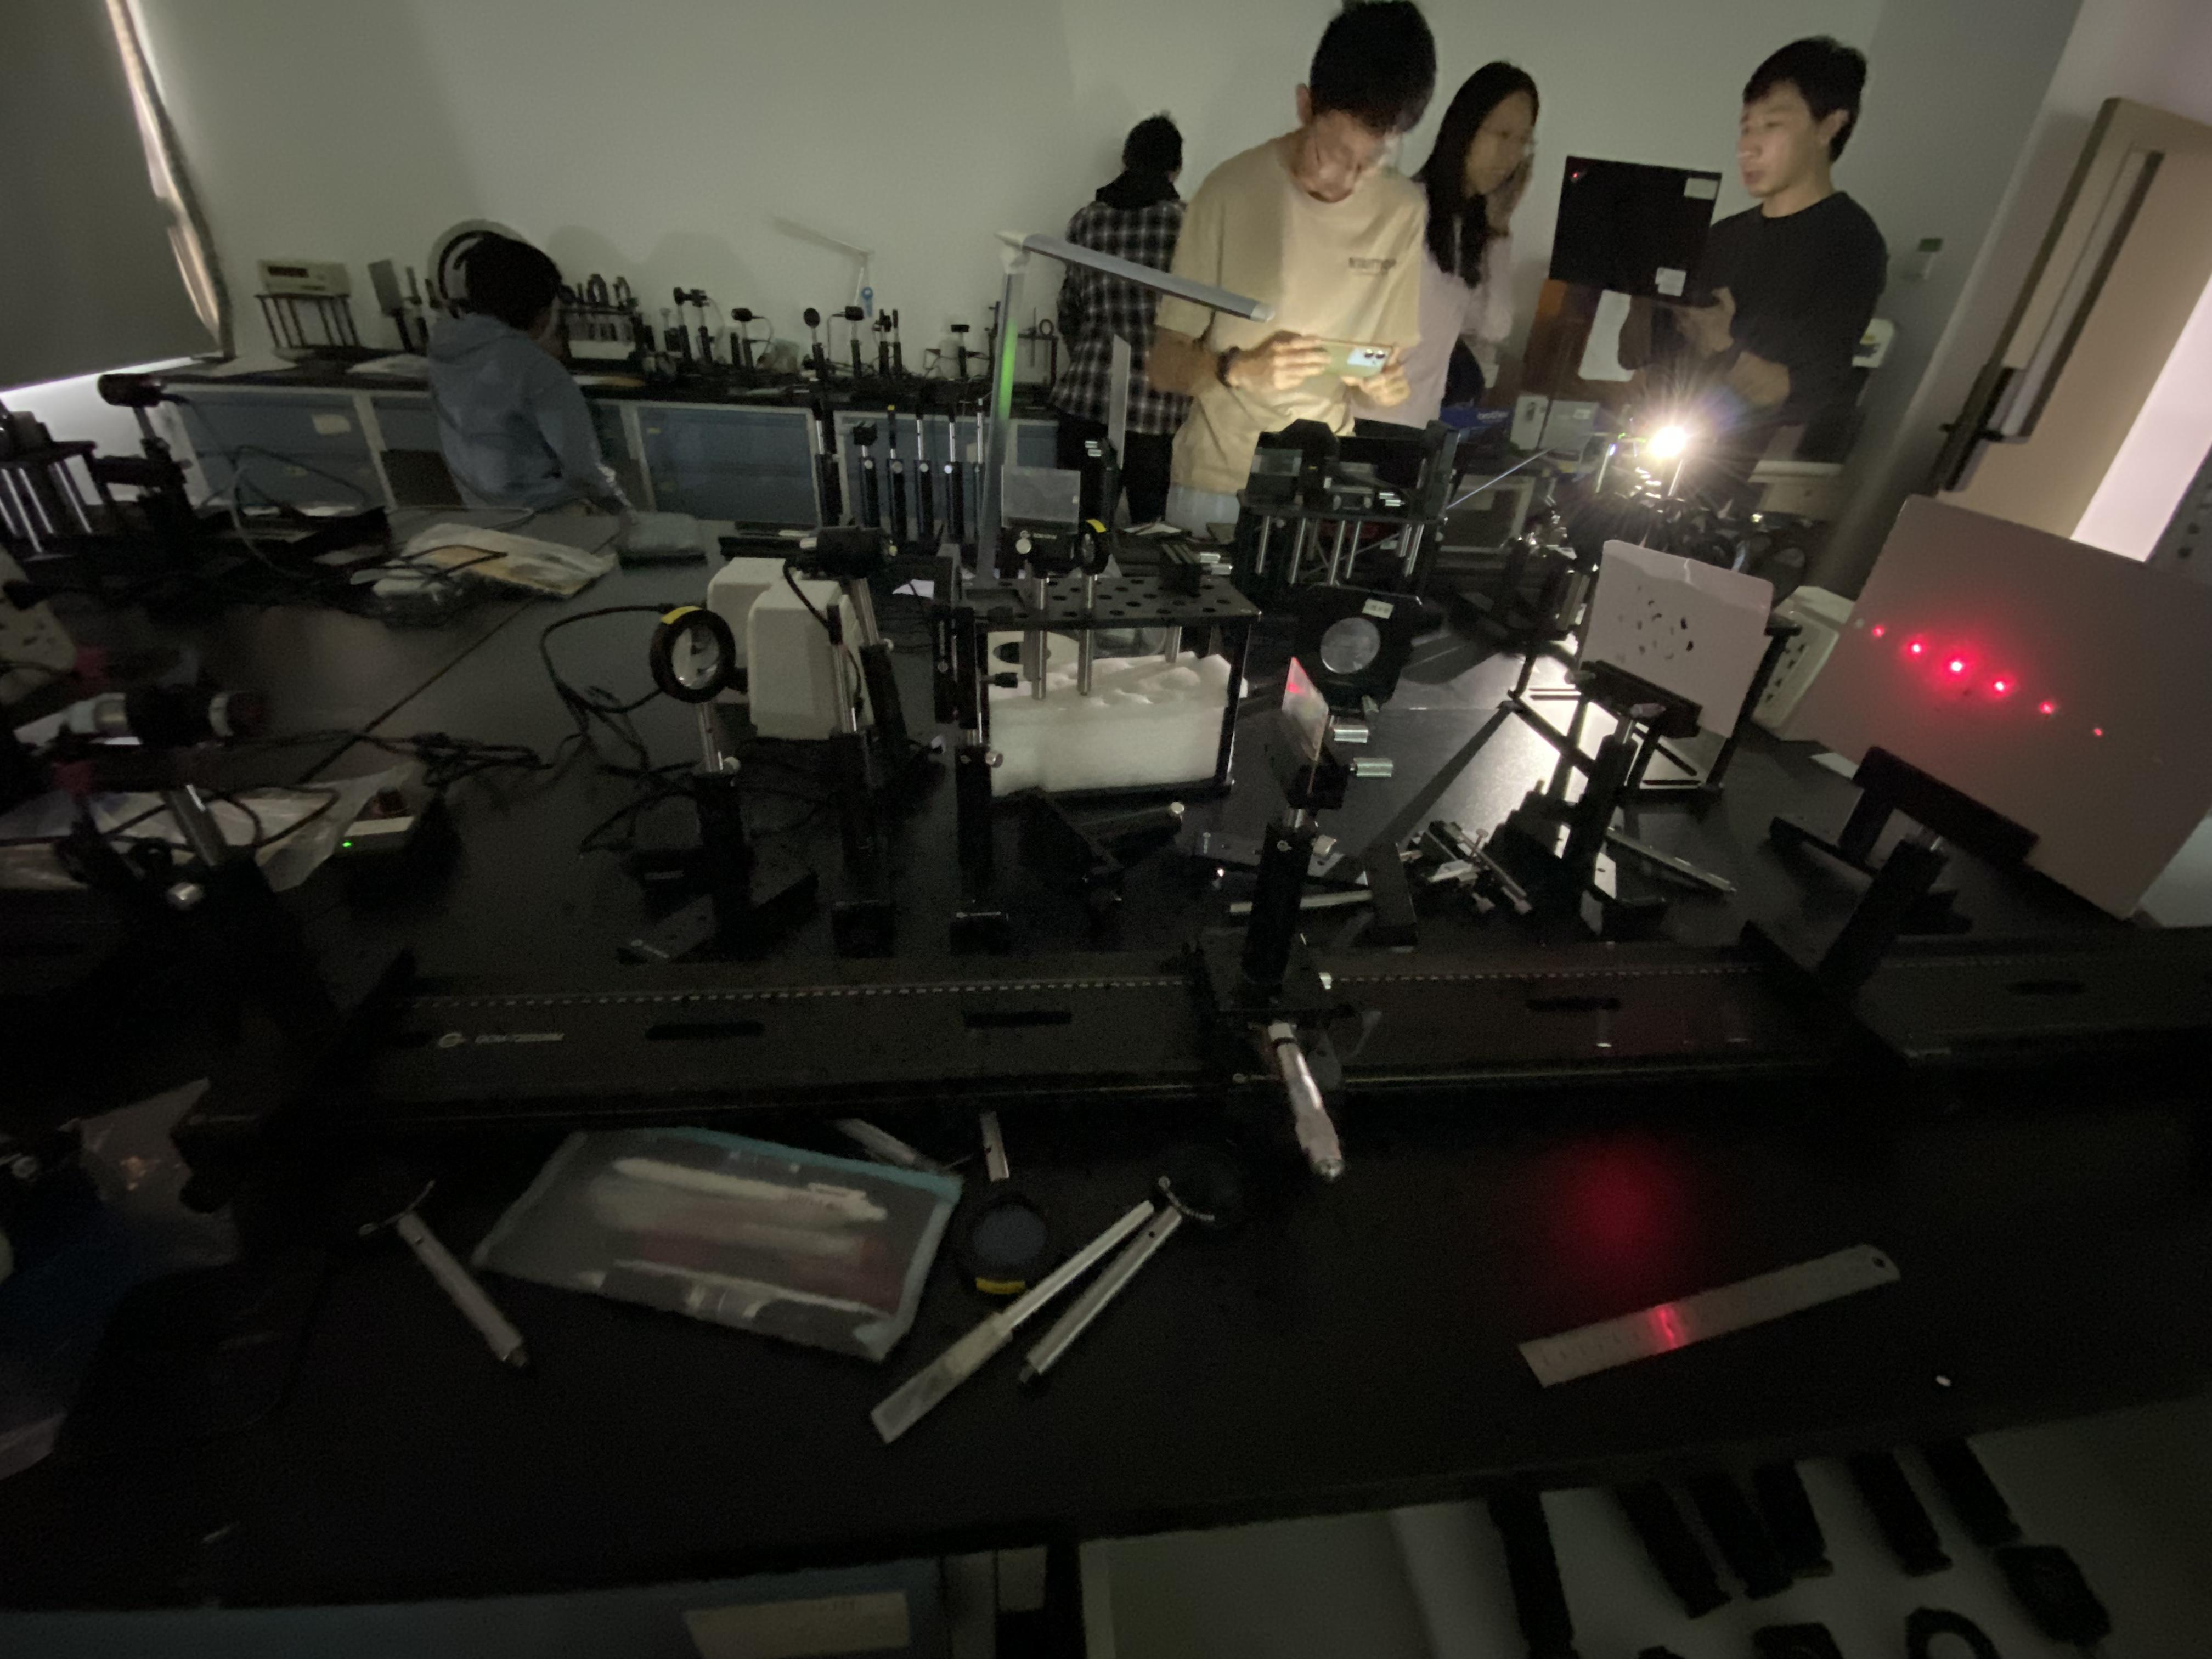
\includegraphics[height=5cm]{./pictures/photos/透射光栅的衍射图样.jpg}
    \caption{透射光栅的衍射图样}
    \label{fig:透射光栅的衍射图样}
  \end{subfigure}
\end{figure}

已知实验用的激光波长为650nm，透射光栅与光屏之间的距离是40cm，零级和一级条纹间距为2.70cm，因此角度的正切值为0.0675。根据光栅方程 \(d \sin \theta_m = m \lambda\)，可以计算出光栅常数 \(d\) 为$9.6\times10^{-6}$m，也就是每毫米有103.8条缝，这与实际值基本吻合。

\subsubsection{实验三：光栅光谱仪测光谱实验}
\begin{figure}[H]
  \centering
  \begin{subfigure}[b]{0.45\textwidth}
    \centering
    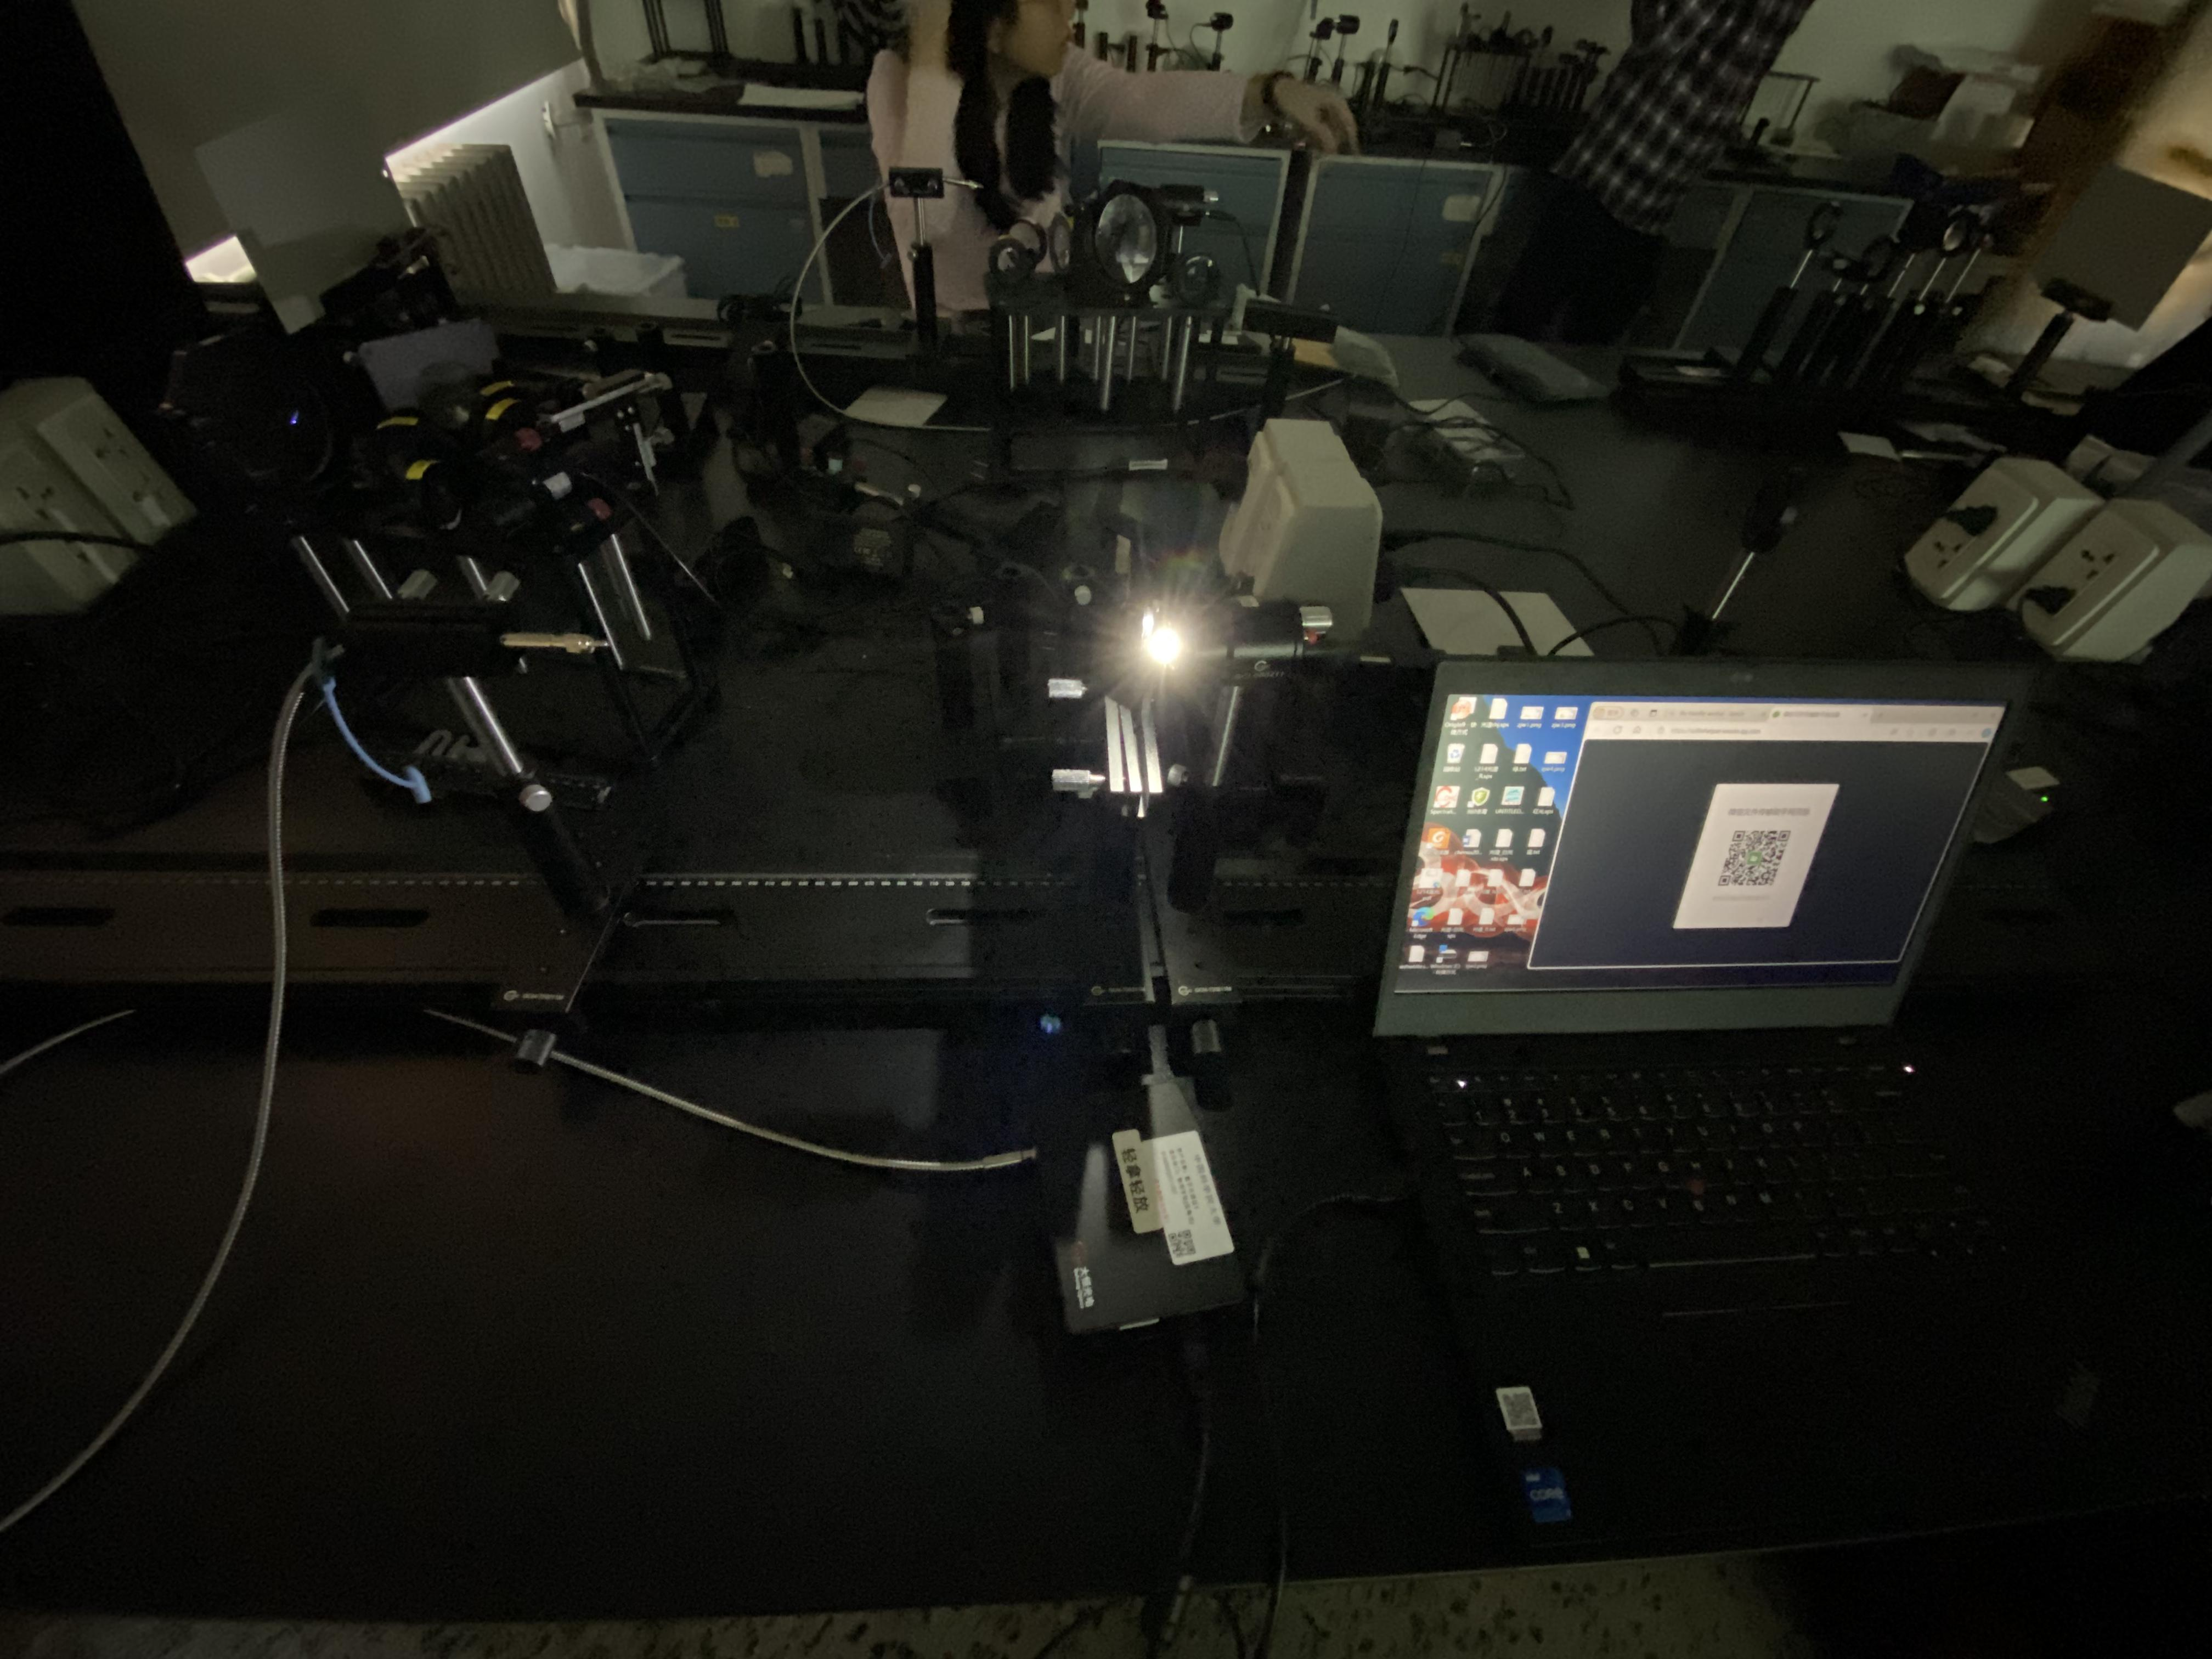
\includegraphics[height=5cm]{./pictures/photos/光栅光谱仪测光谱实验.jpg}
    \caption{光栅光谱仪测光谱实验}
    \label{fig:光栅光谱仪测光谱实验}
  \end{subfigure}
\end{figure}

\begin{figure}[H]
  \centering
  \begin{subfigure}[b]{0.45\textwidth}
    \centering
    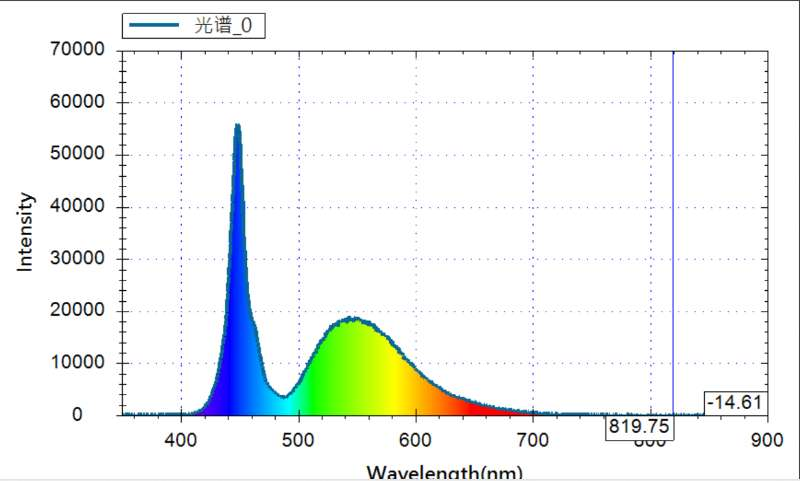
\includegraphics[height=5cm]{./pictures/photos/白光光谱.jpg}
    \caption{白光光谱}
    \label{fig:白光光谱}
  \end{subfigure}
  \hfill
  \begin{subfigure}[b]{0.45\textwidth}
    \centering
    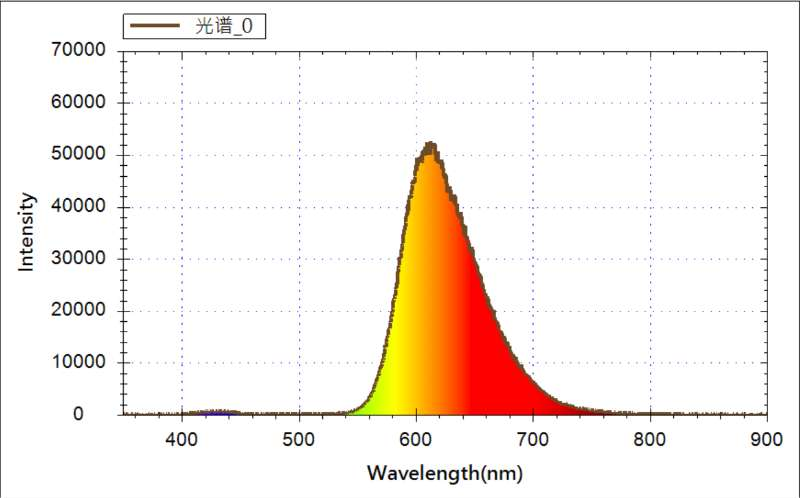
\includegraphics[height=5cm]{./pictures/photos/红光光谱.jpg}
    \caption{红光光谱}
    \label{fig:红光光谱}
  \end{subfigure}
  \label{fig:combined}
\end{figure}

\begin{figure}[H]
  \centering
  \begin{subfigure}[b]{0.45\textwidth}
    \centering
    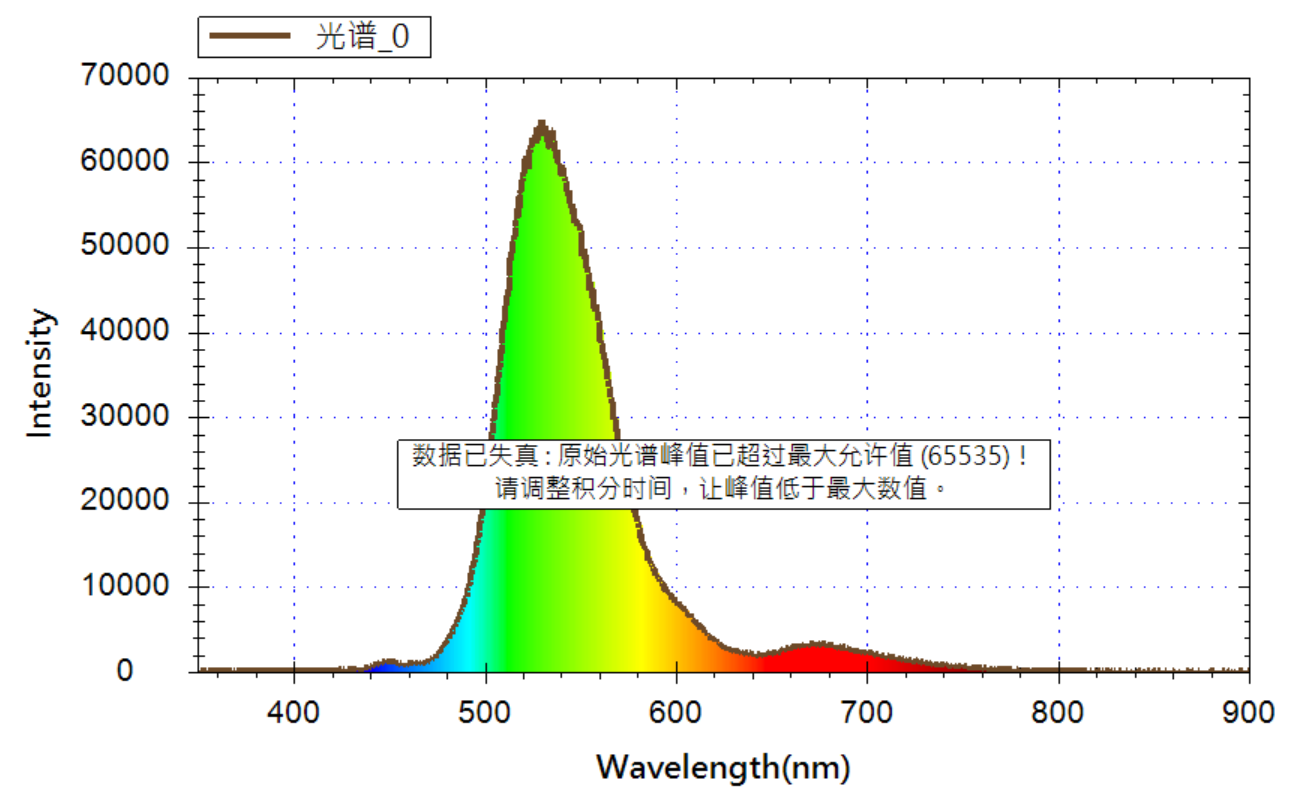
\includegraphics[height=5cm]{./pictures/photos/绿光光谱.png}
    \caption{绿光光谱}
    \label{fig:绿光光谱}
  \end{subfigure}
  \hfill
  \begin{subfigure}[b]{0.45\textwidth}
    \centering
    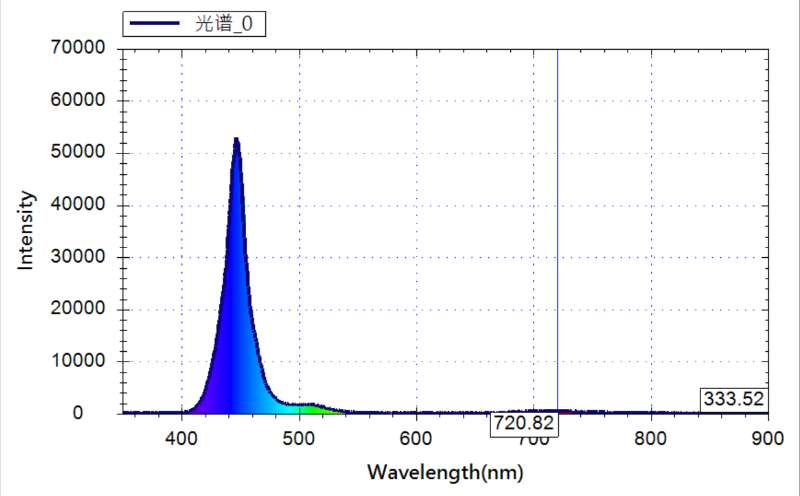
\includegraphics[height=5cm]{./pictures/photos/蓝光光谱.jpg}
    \caption{蓝光光谱}
    \label{fig:蓝光光谱}
  \end{subfigure}
  \label{fig:combined}
\end{figure}

\begin{table}[ht]
    \centering
    \begin{tabular}{|c|c|c|c|}
        \hline
        光源 & 峰值 (nm) & 线宽 (nm) & 中心波长 (nm) \\
        \hline
        白光 & 10099.11 & 90 & 543.10 \\
        红光 & 50543.16 & 72.24 & 618.28 \\
        绿光 & 64682.18 & 62.64 & 530.06 \\
        蓝光 & 56776.66 & 18.1 & 446.59 \\
        \hline
    \end{tabular}
    \caption{不同颜色光的峰值、线宽和中心波长}
    \label{tab:光源参数}
\end{table}

\section{实验总结与思考题}

\subsection{思考题解答}

\textbf{1)} 
\begin{enumerate}
    \item[a)] 阿贝成像中，当“缝”与光栅方向夹角45度放置滤波时，会有何效果？\\
    当“缝”与光栅方向夹角45度放置滤波时，滤波器会选择性地增强或抑制特定方向的光线。最终产生倾斜角度为四十五度的斜条纹。

    \item[b)] 前面实验中，我们使用低通滤波（仅让0级斑通过）实现了光栅格子信息的消除；如何做个高通滤波的例子？应该如何实现和它的效果是什么？\\
    实现一个高通滤波器可以只用一个小圆盘将中心零级点遮住，而使四周边缘的其他频谱点通过。它实现的滤波效果是，光字的图像充满横纵条纹，并且相比于不加滤波片时的像，横纵条纹更清晰，实现了图像的锐化。
\end{enumerate}

\textbf{2)} 观察4F系统成像与阿贝成像时单透镜成像的区别是什么？\\
\indent 4F系统成像与阿贝成像时单透镜成像的区别在于，4F系统利用傅里叶变换的特性，可以有效地将频率成分分开，最终成像的效果更加清晰，可以保存更多的信息。阿贝成像主要依赖于单透镜的光学特性，成像质量受光学畸变和光圈的影响较大。同时，由于4F系统成像四个焦距固定，在搭建实验装置时更加易于操作，容易找到清晰的像。

\textbf{3)} 假彩色编码实验中使用的天安门城楼光栅本身中的城楼的窗户和门洞都是透光的，但是为什么经过所提供的假着色滤波处理后所成的像中这些窗户和门洞是黑色的？有方法验证你的解释吗？\\
\indent 假彩色编码实验中，虽然城楼的窗户和门洞是透光的，但经过假着色滤波处理后，图像中这些部分呈现为黑色，这可能是因为窗户和门洞上的光直接透射，并以几何传播的形式投射在频谱面的中心上，但滤波器中间无开孔，这些光线无法继续传播，因此白屏上的对应位置呈现黑色。如果想要验证这一猜想，可以在自制光栅的中心处开孔，检查所成的像中窗户和门洞处是否有白光透射。

\textbf{4)} 从夫琅和费衍射演示实验得到哪些规律？\\
\indent 从夫琅和费衍射演示实验中可以得到以下规律：
\begin{enumerate}
    \item 当光波通过狭缝或障碍物时，会发生弯曲现象，形成衍射图样。
    \item 夫琅和衍射的模式与光源的波长和孔径的尺寸相关，孔径越小，衍射现象越明显。
    \item 衍射图样的强度的明暗条纹特征与干涉图样不同，他的衰减更快。
    \item 不同形状的孔或障碍物会导致不同的衍射模式。 
\end{enumerate}

\subsection{反思与改进}

\begin{enumerate}
    \item 一开始搭建光路时我并没有严格遵守实验讲义上所写的距离，。在调整光路时，我没有严格按照实验讲义上的步骤进行，导致了实验过程中的困难, 后来多次调整才成功，浪费了很多时间。
    \item 在实验前应提前规划后续步骤，例如在确定光线高度时，应综合考虑各组件的高度，避免出现不协调的情况。
    \item 自制滤波器的时候应该更加细致的标出需要透光的地方，否则滤出的颜色不够理想和准确。
\end{enumerate}

\end{document}

% VScode 常用快捷键：

% F2:                       变量重命名
% Ctrl + Enter:             行中换行
% Alt + up/down:            上下移行
% 鼠标中键 + 移动:           快速多光标
% Shift + Alt + up/down:    上下复制
% Ctrl + left/right:        左右跳单词
% Ctrl + Backspace/Delete:  左右删单词    
% Shift + Delete:           删除此行
% Ctrl + J:                 打开 VScode 下栏(输出栏)
% Ctrl + B:                 打开 VScode 左栏(目录栏)
% Ctrl + `:                 打开 VScode 终端栏
% Ctrl + 0:                 定位文件
% Ctrl + Tab:               切换已打开的文件(切标签)
% Ctrl + Shift + P:         打开全局命令(设置)

% Latex 常用快捷键：

% Ctrl + Alt + J:           由代码定位到PDF


